%% ================================================================
%% TARGET JOURNAL: Chaos, Solitons & Fractals (Elsevier)
%% ISSN: 0960-0779 | Submission: https://www.editorialmanager.com/chaos
%% LaTeX class: Elsevier CAS (review mode for single-column double-spacing submission)
%% Reference style: numbered with author names for \citet support
%% Bibliography source: use the repo-level master .bib to keep citation keys aligned
%% ================================================================
\documentclass[a4paper,fleqn,review]{cas-sc}

%% --- Core packages (natbib and review spacing provided by CAS) ---
\usepackage[utf8]{inputenc}
\usepackage[T1]{fontenc}
\usepackage[english]{babel}
\usepackage[authoryear,longnamesfirst]{natbib}
\usepackage{amsmath,amssymb,amsfonts}
\usepackage{graphicx}
\usepackage{hyperref}
\usepackage{url}
\usepackage{booktabs}
\usepackage{multirow}
\usepackage{subcaption}
\usepackage{algorithm}
\usepackage{algorithmic}
\usepackage{float}
\usepackage{placeins}
\usepackage{rotating}
\usepackage{indentfirst}

\flushbottom

% Keep float-only pages top-aligned; do not center a figure in a large white
% area when the surrounding text cannot fit on the preceding page.
\makeatletter
\setlength{\@fptop}{0pt}
\setlength{\@fpbot}{0pt plus 1fil}
\makeatother

\setlength{\textfloatsep}{10pt plus 2pt minus 2pt}
\setlength{\floatsep}{8pt plus 2pt minus 2pt}
\setlength{\intextsep}{8pt plus 2pt minus 2pt}
\setcounter{topnumber}{2}
\setcounter{bottomnumber}{2}
\renewcommand{\topfraction}{0.95}
\renewcommand{\bottomfraction}{0.85}
\renewcommand{\textfraction}{0.05}
\renewcommand{\floatpagefraction}{0.55}

%% Figure width/height guardrails
\newcommand{\paperfigwidth}{\textwidth}
\newcommand{\paperfigheight}{0.74\textheight}

%% hyperref customisation
\hypersetup{
    colorlinks=true,
    linkcolor=blue,
    filecolor=magenta,
    urlcolor=cyan,
    citecolor=blue
}

\begin{document}
\let\WriteBookmarks\relax
\def\floatpagepagefraction{1}
\def\textpagefraction{.001}

\shorttitle{Taxonomy of Critical Phenomena in Financial Markets}
\shortauthors{Cardoso and Sato}
\title[mode = title]{Taxonomy of Critical Phenomena in Financial Markets}

\author[1]{Gerson Nassor Cardoso}
\cormark[1]
\fnmark[1]
\ead{gersonnassor@gmail.com}
\credit{Conceptualization, Methodology, Software, Formal analysis, Data curation, Visualization, Writing -- original draft}

\author[1]{Renato Cesar Sato}
\ead{rcsato@unifesp.br}
\credit{Supervision, Validation, Writing -- review \& editing}

\affiliation[1]{organization={Graduate Program in Technological Innovation (PPG-PIT), Universidade Federal de S\~{a}o Paulo (UNIFESP)},
            city={S\~{a}o Paulo},
            country={Brazil}}
\cortext[1]{Corresponding author}
\orcidauthor{0000-0002-8499-3390}{Gerson Nassor Cardoso}
\orcidauthor{0000-0002-9902-9086}{Renato Cesar Sato}

%% ----------------------------------------------------------------
%% ABSTRACT ? CSF recommends = 250 words (concise, factual, no refs)
%% ----------------------------------------------------------------
\begin{abstract}
This study examines market-interdependence changes in rolling correlation networks of Brazilian equities (B3). We analyze 360 monthly rolling windows from 1995 to 2025 using hierarchical clustering and planar maximally filtered graphs. The operational panel contains 25 metrics: distance moments, planar mesoscopic measures, eleven Forman--Ricci edge-curvature distribution statistics, size-conditioned group and centrality residuals, and KS/MP matrix diagnostics. We evaluate these metrics around four configured core stress events and use seven supplementary sensitivity anchors, comprising one additional $-3\sigma$ trigger and six fallback proxies. Across the four core events, event-containing windows show lower mean PMFG distance and higher KS displacement and MP signal variance relative to local pre-event phases. Lower mean PMFG distance also persists post-event, whereas curvature, community, group, and centrality responses are event-specific. The framework provides a descriptive rolling architecture for comparing 25-metric configurations around externally dated stress anchors without implying causality or prediction.
\end{abstract}

% Highlights are a deliberately sparse CAS front-matter page; do not stretch
% their inter-item spacing to the footer.
\raggedbottom
\begin{highlights}
\item A 25-metric rolling architecture tracks B3 topology across 360 windows.
\item PMFG distances and spectral concentration change at four core events.
\item Size-conditioned residuals separate topology from the changing B3 universe.
\item Four event phases reveal recurring and episode-specific configurations.
\item The evidence supports descriptive monitoring, not causal prediction.
\end{highlights}

%% ----------------------------------------------------------------
%% KEYWORDS ? 4?7 terms separated by \sep
%% ----------------------------------------------------------------
\begin{keywords}
systemic risk \sep B3 \sep financial networks \sep PMFG \sep spectral diagnostics
\end{keywords}
\maketitle
\raggedbottom

\section{Introduction}
\label{sec:introduction}

\subsection{Relevance}

We characterize financial crises not merely as episodes of elevated volatility; rather, they constitute periods in which the structure of interdependence across assets changes qualitatively. Markets that appear diversified during tranquil conditions often become structurally compressed under stress, with cross-sector comovement increasing, previously separated groups merging, and a small subset of nodes concentrating a disproportionate share of systemic importance. This perspective is consistent with the literature on financial correlation networks and market topology, which indicates that crises are associated with abrupt changes in hierarchical organization, network centrality, and cluster persistence rather than merely higher average correlations \citep{mantegna1999hierarchical,tumminello2010correlation,musmeci2015risk}.

Research on systemic risk and financial connectedness further argues that fragility emerges through dynamic topological reconfiguration, contagion pathways, and time-varying dependency structures that are not fully captured by conventional volatility indicators or static covariance summaries \citep{billio2012econometric,bardoscia2017pathways}. More recent studies reinforce this interpretation by showing that multilayer spillovers, heterogeneous dependency channels, and evolving network topology contain relevant information about systemic transitions and crisis propagation, with evidence spanning econophysics, complex-systems finance, and network-based diagnostics of systemic-risk monitoring \citep{das2025covar,an2025regimeswitching,silva2016structure,huang2018systemic,ma2019diversification,alexandre2021drivers,clemente2022multilayer}.

For supervisors, regulators, and portfolio managers, the key question is therefore not only whether correlations increase, but how market structure reorganizes before, during, and after stress. Prior work suggests that transitions between market regimes are frequently accompanied by compression of network distances, synchronization among sectors, changes in centrality concentration, and reorganization of community structures, indicating that topology itself may contain early-warning information about systemic instability \citep{musmeci2015risk,billio2012econometric}. Consequently, understanding how clusters emerge, collapse, persist, and reconnect across market regimes has become increasingly relevant for financial monitoring, risk management, and macroprudential supervision.

Within this practical context, the study organizes observations into four operational rolling-window states: a tranquil reference, local pre-event, crisis, and post-event reorganization state. The externally configured shock date is a rupture marker between the pre-event and crisis states, not a fifth state. The aim is not to infer which metric causes or predicts a crisis. Instead, the taxonomy provides a transparent exploratory map of how the same structural diagnostics co-vary across local comparisons after discounting the changing asset universe. This supports cautious market monitoring and contributes a reproducible descriptive architecture for studying structural transitions in complex adaptive systems.

\subsection{Research Context and Gap}

Financial-network research has established that dependence is geometrically structured and time-varying. Correlation matrices can be transformed into metric distances that reveal hierarchical organization \citep{mantegna1999hierarchical}; subsequent studies documented temporal reorganization during stress and developed filtered representations for dynamic market analysis \citep{onnela2003dynamics,tumminello2005tool,tumminello2007hierarchically,sandoval2015structure}. These contributions motivate a multi-scale treatment of market structure rather than a reliance on volatility or pairwise correlation summaries alone.

The PMFG is particularly useful for this purpose because it retains more edges, cycles, and mesoscopic organization than a minimum spanning tree while preserving planarity \citep{tumminello2005tool,nobi2017systemic}. Its use allows locally expressed B3 stress episodes to be examined as changes in dependence structure rather than as volatility events alone. The present study keeps the four core crashes externally configured and treats locally selected anchors only as descriptive sensitivity cases.

The literature on critical transitions and early-warning signals motivates examining changes in variance, synchronization, community structure, and spectral concentration \citep{scheffer2009earlywarning,billio2012econometric,an2025regimeswitching}. However, the present study does not estimate recovery rates, test a predictive pre-transition signature, or claim a universal crisis sequence. The remaining gap is methodological: long-horizon rolling protocols that jointly compare hierarchical partitions, planar topology, size-conditioned diagnostics, and spectral structure across multiple dated B3 stress episodes remain limited. The present paper addresses this gap with a retrospective descriptive taxonomy.

\subsection{Problem Statement}

Despite advances in financial-network analysis, most operational monitoring stacks still emphasize pairwise summaries and volatility diagnostics, with limited structural interpretation of how clusters emerge, collapse, and reconnect across regimes. Correlation matrices, covariance estimates, rolling volatilities, and stress indicators remain central to market surveillance infrastructures, yet several studies have noted that such approaches provide only partial visibility into the evolving organization of financial systems, particularly during periods of instability \citep{mantegna1999hierarchical,tumminello2010correlation}.

The literature on financial networks and hierarchical clustering argues that monitoring topology --- including community persistence, centrality shifts, contagion pathways, and structural fragmentation --- can reveal dimensions of systemic risk that remain obscured in aggregate statistical indicators \citep{musmeci2017bootstrapping,bardoscia2017pathways}. However, many practical monitoring frameworks still operationalize market dependence primarily through pairwise correlation summaries, without explicitly modeling the evolution of higher-order structural organization.

This study addresses that gap by focusing explicitly on the evolution of market topology across stress regimes, emphasizing interpretable measures of cluster formation, persistence, reconnection, distance redistribution, and centrality reallocation.

\subsection{Hypothesis}

We examine whether the four pre-specified B3 crashes are associated with a multi-metric structural reconfiguration across tranquil, pre-crisis, event-containing, and post-crisis windows. Operationally, this entails joint changes in hierarchical partitions, PMFG distances and modularity, centralities, and spectral structure after discounting the changing eligible universe; it does not posit a common directional signature for every metric.

A secondary sensitivity hypothesis is that locally selected B3 stress anchors may exhibit heterogeneous structural variation associated with local events, shocks, or crash episodes. This expectation is motivated by the institutional and political instability observed over the long B3 history, the availability of a sufficiently long and liquid data record, and evidence that electoral periods can coincide with reorganization of the B3 correlation network \citep{cardoso2022electoral}. The eleven-anchor calendar therefore tests whether the configurations observed around the four core events also recur, with local variation, around one additional $-3\sigma$ trigger and six fallback local-drop anchors. This is a descriptive robustness hypothesis: it does not assign a political or other historical cause to any anchor, and it does not treat the fallback anchors as confirmed crashes or predictive signals.

\subsection{Objectives}


This paper studies structural reorganization in financial markets through a rolling pipeline that uses B3 as its empirical case and integrates two complementary views of market organization:
\begin{enumerate}
    \item A hierarchical view, based on correlation matrices, heatmaps, and dendrograms, to map how groups form and dissolve.
    \item A topological view, centered on planar financial networks, to quantify modularity, community structure, centrality concentration, and distance-distribution reconfiguration.
\end{enumerate}

To make the manuscript's novelty operationally explicit, we summarize four concrete contributions. First, a planar-first rolling architecture that avoids significance-thresholded backbone pruning at the network-construction stage, preserving structural comparability across windows. Second, a joint hierarchical-topological diagnostic stack that maps the same regime transition through independent objects (clusters, planar communities, centrality concentration, and distance moments). Third, an explicit size-conditioned control that separates changes in structural diagnostics from the expanding eligible universe. Fourth, a reproducible long-horizon evidence base (1995--2025) that compares tranquil, pre-crisis, event-containing, and post-crisis configurations around four severe B3 drawdowns.

The framework is explicitly multi-scale, combining pairwise dependence, mesoscopic clustering, and global topological organization into a unified rolling architecture. The substantive focus is planar. Complete graphs are too dense for structural interpretation, and the MST suppresses cycles and mesoscopic motifs that are crucial for crisis analysis. Relative to the MST, PMFG networks retain more edges while preserving planarity, capturing local cycles and richer mesoscopic organization. For this reason, the central structural interpretation is built on planar networks.

The novelty of the paper lies not in proposing isolated metrics, but in integrating hierarchical clustering, planar topology, and spectral diagnostics into a unified rolling framework capable of tracking structural regime transitions in B3 over three decades. The goal is not point forecasting of returns or volatility, nor causal identification of crises, but structural characterization of evolving market organization and systemic vulnerability. The article contributes by: (i) documenting a reproducible planar-first pipeline for systemic monitoring, (ii) applying a common size-conditioned control to the cross-window comparisons reported quantitatively, including centralities, and (iii) organizing the evidence as a descriptive tranquil/pre-crisis/during/post-crisis regime taxonomy.

From the perspective of nonlinear and complex-systems science, the central interest of this paper lies in the characterization of abrupt structural transitions in financial correlation networks. The analysis does not assume that all crises follow an identical topological path. Instead, it compares their joint configurations across several complementary diagnostics and identifies which components recur and which remain episode-specific. This connects the study to the econophysics tradition that treats financial markets as complex adaptive systems \citep{mantegna1999hierarchical,stanley1996scaling}.

\section{Data and Empirical Architecture}
\label{sec:data_methodology}

\subsection{Financial Universe and Rolling Windows}

The financial universe is composed of liquid B3 equities observed in rolling windows of approximately one year with monthly updates, producing 360 windows spanning January 1995 to November 2025 --- a 30-year history of the Brazilian equity market. The rolling universe is dynamic rather than fixed, reflecting the historical evolution of B3 liquidity conditions and avoiding survivorship bias associated with retrospectively selecting only currently listed firms. Eligibility is determined by an explicit asset-selection pipeline rather than by ex post convenience. The filter retains only local equity classes admitted by the B3/CVM mapping, applies minimum effective-trading completeness and frequency thresholds of 80\% over the asset's observed life, imposes a minimum average-volume requirement, and restricts the universe to admissible share classes (ON, PN, and units). To avoid double-counting the same firm through multiple concurrent classes, the pipeline keeps a single security per company, prioritizing PN over ON and ON over units, with volume used as a tie-breaker within class. Additional quality controls remove corrupted ticker records, harmonize legacy symbols, consolidate duplicate date--ticker observations, and enforce minimum within-window presence before the rolling correlation stage. Each window advances by one calendar month, and asset coverage grows substantially across the sample: from 11 liquid equities in the earliest windows, when only a handful of B3 stocks had sufficient price history and passed the eligibility rules, to approximately 178 equities in the most recent windows as the exchange expanded and liquidity standards deepened. This expansion is reflected directly in planar-graph richness: early windows are structurally sparse, while later windows exhibit substantially denser PMFG topologies as the tradable universe matures.

The sample spans multiple macro-financial regimes, including the post-Real stabilization period, the 1999 currency crisis, the Global Financial Crisis, the Brazilian sovereign and political crises of the mid-2010s, the COVID-19 shock, and the subsequent geopolitical turbulence linked to the Russia--Ukraine war. This temporal breadth is important because the paper is designed to compare how network structure reacts under distinct external and domestic stress configurations rather than within a single historical episode.

Daily adjusted closing prices are sourced from the official B3/BM\&FBovespa historical quotation series (COTAHIST). Data were downloaded from \url{https://bvmf.bmfbovespa.com.br/InstDados/SerHist/}. For each window, adjusted closing prices are transformed into log returns,
\begin{equation}
r_{i,t} = \ln P_{i,t} - \ln P_{i,t-1},
\label{eq:log-return}
\end{equation}
and pairwise Pearson correlations are estimated over the window according to the standard rolling correlation-network setup used in the financial-network literature~\citep{tumminello2010correlation},
\begin{equation}
\rho_{ij}(t) = \frac{\sum_{\tau \in \mathcal{W}_t} \bigl(r_{i,\tau} - \bar{r}_{i,t}\bigr)\bigl(r_{j,\tau} - \bar{r}_{j,t}\bigr)}{\sqrt{\sum_{\tau \in \mathcal{W}_t} \bigl(r_{i,\tau} - \bar{r}_{i,t}\bigr)^2} \, \sqrt{\sum_{\tau \in \mathcal{W}_t} \bigl(r_{j,\tau} - \bar{r}_{j,t}\bigr)^2}},
\label{eq:pearson-correlation}
\end{equation}
where $\mathcal{W}_t$ denotes the set of observations inside rolling window $t$, and $\bar{r}_{i,t}$ is the mean return of asset $i$ within that window. The use of overlapping windows balances temporal sensitivity and statistical stability: the windows are short enough to track transitions around crises, yet long enough to support meaningful correlation and clustering estimates.

The pipeline stores each window with explicit start and end dates and treats windows as operational units. This window-based organization is essential for crisis analysis because the empirical comparisons are conducted locally around stress episodes, allowing the paper to track how correlation groups and planar topology reorganize in the months immediately before and after major market shocks.


\subsection{Empirical Architecture}

We introduce an empirical architecture consisting of two complementary analytical layers: hierarchical clustering and planar topology (PMFG). The central object of analysis is structural regime transition: the progressive reorganization of market topology that precedes, accompanies, and follows systemic stress episodes.

Within this framework, structural reconfiguration denotes changes in modular separation, distance distribution, and centrality allocation relative to the evolving eligible universe. The analysis compares these quantities across tranquil, pre-crisis, event-containing, and post-crisis windows without equating any one diagnostic with systemic fragility.

\subsection{From Correlation Matrices to Financial Distances}

For each window, the correlation matrix $\mathbf{R}(t)$ is transformed into a distance matrix using the metric transformation introduced by \citet{mantegna1999hierarchical}
\begin{equation}
d_{ij}(t) = \sqrt{2(1-\rho_{ij}(t))}.
\label{eq:financial-distance}
\end{equation}
This mapping preserves the metric structure used in the seminal correlation-network literature: perfectly positively correlated pairs satisfy $d_{ij}=0$, uncorrelated pairs satisfy $d_{ij}=\sqrt{2}$, and perfectly negatively correlated pairs satisfy $d_{ij}=2$. Hence, negative correlations are assigned large distances, so anti-correlated assets are treated as remote from one another in the same geometric sense adopted by \citet{mantegna1999hierarchical}. In hierarchical and planar representations this implies that negatively correlated pairs tend to appear as long-range or peripheral relations rather than as tight local neighbors. The distance representation therefore links the matrix view to the network view while retaining the economic interpretation that stronger positive comovement corresponds to geometric proximity.

\subsection{Statistical Backbone and Hierarchical Clustering}

Under the null hypothesis of zero correlation, the pairwise test statistic is $t_{ij} = \rho_{ij}\sqrt{\frac{W-2}{1-\rho_{ij}^2}}$, which follows a Student-$t$ distribution with $W-2$ degrees of freedom. The pipeline computes $p$-values for annotation only: edges with $p < 0.05$ are drawn as solid lines; edges with $p \geq 0.05$ as dashed. The PMFG is constructed from the \emph{full} distance matrix without significance filtering, preserving all topologically relevant connections.

For hierarchical clustering, the distance matrix is submitted to agglomerative clustering using average linkage. The selected number of groups is determined by maximizing the silhouette score within an admissible range. In the hierarchical block, group counts are interpreted through a size-adjusted baseline that removes first-order effects of sample size, allowing comparison of segmentation across windows of different tradable universe sizes. The pipeline also stores modularity diagnostics for each partition: $Q=\frac{1}{2m}\sum_{i,j}(A_{ij}-\frac{k_i k_j}{2m})\mathbf{1}\{c_i=c_j\}$, where $A_{ij}$ is adjacency weight and $2m=\sum_{ij}A_{ij}$ is total weight.

For the planar community count, the empirical size-conditioned baseline is
\begin{equation}
\label{eq:size_only_null}
\widehat{C}_t=\alpha+\beta\log(1+N_t),
\end{equation}
where $N_t$ is the number of eligible nodes in window $t$ and the residual is $C_t-\widehat{C}_t$. For continuous planar diagnostics, the corresponding control is
\begin{equation}
\label{eq:size_only_topology_null}
\widehat{X}_t=a_X+b_X\log(1+N_t),\qquad \eta_t=X_t-\widehat{X}_t.
\end{equation}
These are empirical size-conditioned controls, not structural null models for the PMFG algorithm; they are used only to separate cross-window comparisons from first-order changes in the eligible universe.

\subsection{Planar Financial Networks}

The second analytical family is topological. The PMFG is constructed from the \emph{full} distance matrix for each window: all candidate edges are ranked by ascending distance and added iteratively, each subject to the linear-time Boyer--Myrvold planarity check. An edge is retained if and only if its inclusion preserves planarity; the process terminates when no further edge can be incorporated without violating this constraint, or when the structural maximum of $3N-6$ edges is reached. The planarity constraint alone defines the topological backbone, preserving mesoscopic loops and redundant transmission paths that a minimum-spanning-tree representation would eliminate. The p-values computed in the preceding subsection serve solely as visual annotation: non-significant edges are rendered as dashed lines in planar-network snapshots, allowing statistical confidence to be read directly from the figure without altering the structural construction.

The tradable universe in early sample windows (approximately 1995--2000) contained a limited number of liquid B3 equities with sufficient return history. Planar graphs in this period therefore carry fewer edges, reflecting genuine data sparsity rather than a pipeline artifact. As the exchange expanded and liquidity conditions deepened after 2000, planar topologies became progressively richer and structurally more informative.

On the planar graph we track average degree, density, community structure, centrality moments, modularity, and the empirical moments of financial distances. This extends to a planar backbone the dynamic financial-network logic popularized for correlation trees by \citet{onnela2003dynamics}, but without collapsing the market into a tree. For the distance layer, the pipeline stores the four moments of the PMFG edge-distance distribution in each window: mean, variance, skewness, and kurtosis,
\begin{equation}
\label{eq:distance_moments}
\mu_d=\frac{1}{M}\sum_{e=1}^{M} d_e,
\end{equation}
\subsection{Operational Validation}

The pipeline also retains a random-matrix validation layer, alongside ADF summaries, clustering diagnostics across methods, coverage-control tables, and crisis-window summaries. Concretely, each rolling window is checked against a Gaussian null through a two-sample KS comparison on correlation entries and through a Marchenko--Pastur spectral decomposition of the empirical correlation matrix. These outputs are not peripheral; they establish that the visual narrative is grounded in recurring rolling evidence rather than in a small set of selected crisis anecdotes.

For each rolling window, a non-parametric Kolmogorov--Smirnov (KS) test evaluates whether the empirical pairwise-correlation structure differs from a Gaussian null. A matrix of i.i.d.\ $\mathcal{N}(0,1)$ returns with the same dimensions ($W \times N$) as the empirical window is drawn independently for each window; its Pearson correlation matrix is computed, and a two-sample KS test~\citep{kolmogorov1933,smirnov1948} is applied between the upper-triangular entries of the empirical and null correlation matrices. Denoting by $\mathcal{R}_t$ the empirical upper-triangular correlation sample and by $\mathcal{R}^{(0)}_t$ the Gaussian-null counterpart, the validation statistic is

\begin{equation}
\label{eq:ks_statistic}
D_t = \sup_x \left| \widehat{F}_{\mathcal{R}_t}(x) - \widehat{F}_{\mathcal{R}^{(0)}_t}(x) \right|,
\end{equation}

\noindent where $\widehat{F}$ denotes the empirical cumulative distribution function. Under the null hypothesis, the empirical and Gaussian-null correlation-entry distributions are identical. A near-zero KS $p$-value rejects this distributional equality, indicating rolling dependence structure that differs from the simulated noise benchmark. ADF stationarity tests on each return series provide a complementary check that the windows feed stationary inputs to the correlation estimator.

As a second spectral diagnostic, Random Matrix Theory (RMT) is applied through the Marchenko--Pastur law. For a window with $W$ observations and $N$ assets, the upper bulk edge is

\begin{equation}
\label{eq:mp_upper}
\lambda_+ = \sigma^2 \!\left(1 + \sqrt{q}\,\right)^2, \quad q = \frac{N}{W},
\end{equation}

\noindent where $\sigma^2 = 1$ for a correlation matrix~\citep{marchenko1967,laloux1999noise,plerou2002random}. Empirical eigenvalues above $\lambda_+$ carry cross-sectional information; those at or below $\lambda_+$ are statistically indistinguishable from noise generated by the finite-sample ratio $q$. In the Brazilian context, Aires and Crepaldi examine correlation structure during the Asian and 2008 financial-crisis periods, providing directly related RMT context for the externally dated crisis windows studied here~\citep{aires2022brazilrmt}. Related applications in Tunisia and Spain provide further emerging- and developed-market contexts for the spectral layer~\citep{benyaala2025tunisiarmt,dominguezmonterroza2025spanishrmt}. For each window, the pipeline records the fraction of total variance attributable to signal eigenvalues ($\lambda_i > \lambda_+$), denoted $\widehat{f}_{\text{signal}}$, and the fraction attributable to the dominant (market) eigenvalue $\lambda_1$, denoted $\widehat{f}_{\text{mkt}}$:

\begin{equation}
\label{eq:mp_signal_frac}
\widehat{f}_{\text{signal},t}=\frac{\sum_{i:\,\lambda_i>\lambda_+}\lambda_i}{\sum_{i=1}^N \lambda_i},
\qquad
\widehat{f}_{\text{mkt},t}=\frac{\lambda_1}{\sum_{i=1}^N \lambda_i}.
\end{equation}

\section{Workflow Summary}


The rolling workflow can be summarized concisely. For each window, returns are converted into a correlation matrix and then into financial distances. From that common input, the framework generates two analytical layers: a hierarchical layer (heatmaps, dendrograms, and clustering diagnostics) and a planar layer (PMFG topology, communities, centralities, and distance moments). These layers are then integrated through rolling cross-metric associations and crisis-window comparisons, yielding a unified set of structural regime diagnostics.

\section{Results}
\label{sec:results}

The results first describe all 360 rolling windows through correlation-matrix, hierarchical, and PMFG diagnostics. They then compare the four pre-specified events using a tranquil benchmark and local pre-event, event-containing, and post-event phases. Distance moments and modularity are reported as raw descriptive context; Ward groups and centralities use size-adjusted residuals; KS and Marchenko--Pastur quantities characterize the correlation-matrix layer.

\subsection{Validation of Rolling Windows and Clustering Choices}
\label{subsec:validation}

Figure~\ref{fig:ks-mp-evolucao} reports the 360-window trajectories of the KS statistic and the two MP variance fractions, with the configured event dates overlaid. The KS statistic measures departure from the Gaussian-null correlation benchmark; the MP fractions separate variance in the dominant market mode from variance in all signal eigenvalues. The Ward best-$k$ trajectory is retained as supplementary validation in Appendix~C.

\begin{center}
\captionsetup{type=figure}
\centering
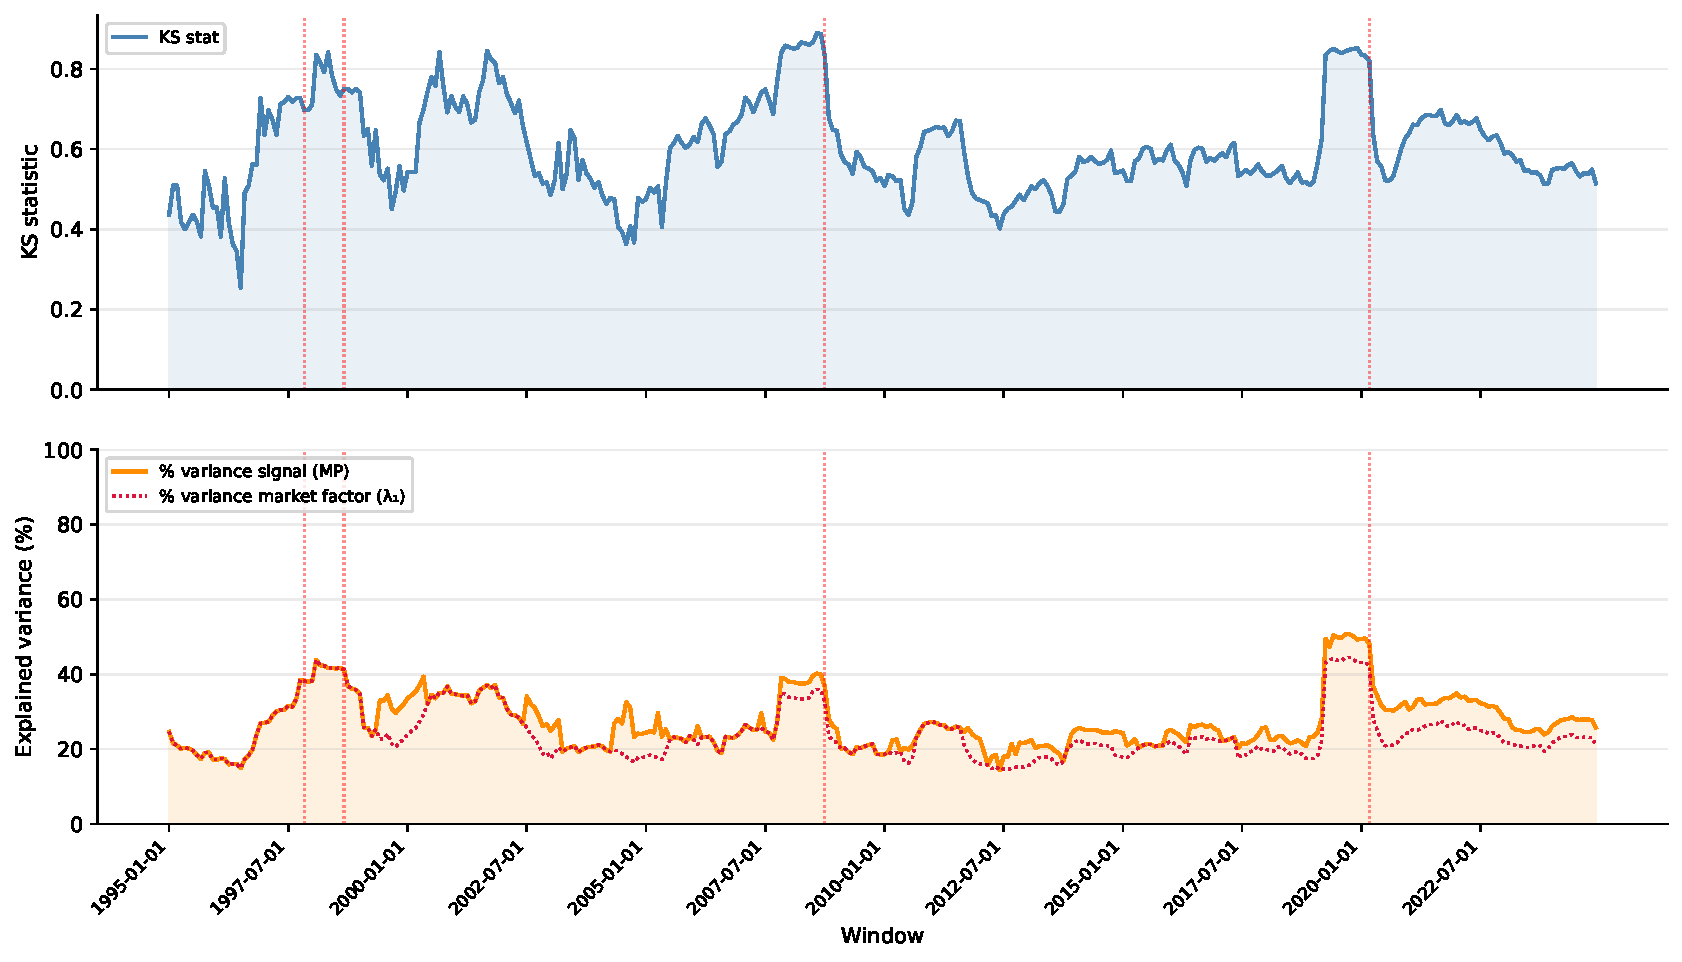
\includegraphics[width=\linewidth,keepaspectratio]{figures/validation/ks_mp_evolucao.pdf}
\caption[KS and Marchenko--Pastur diagnostics]{Rolling KS statistic and Marchenko--Pastur diagnostics over the 360-window history. The all-event comparison finds increased KS displacement, MP signal variance, and market-mode fraction in the event-containing phase of all four configured crashes; post-event market-mode changes are less concordant.}
\label{fig:ks-mp-evolucao}
\end{center}

The visual validation panel should be read as a joint diagnostic block. The KS curve identifies departures from the Gaussian reference, whereas the two MP fractions distinguish broad signal variance from concentration in the leading market mode. The best-$k$ curve is not interpreted independently: its role is to document the changing hierarchical partition used by the subsequent size-conditioned group comparisons.

The silhouette and clustering-modularity curves provide supporting diagnostics for the quality and continuity of the Ward partition.

\begin{center}
\captionsetup{type=figure}
\centering
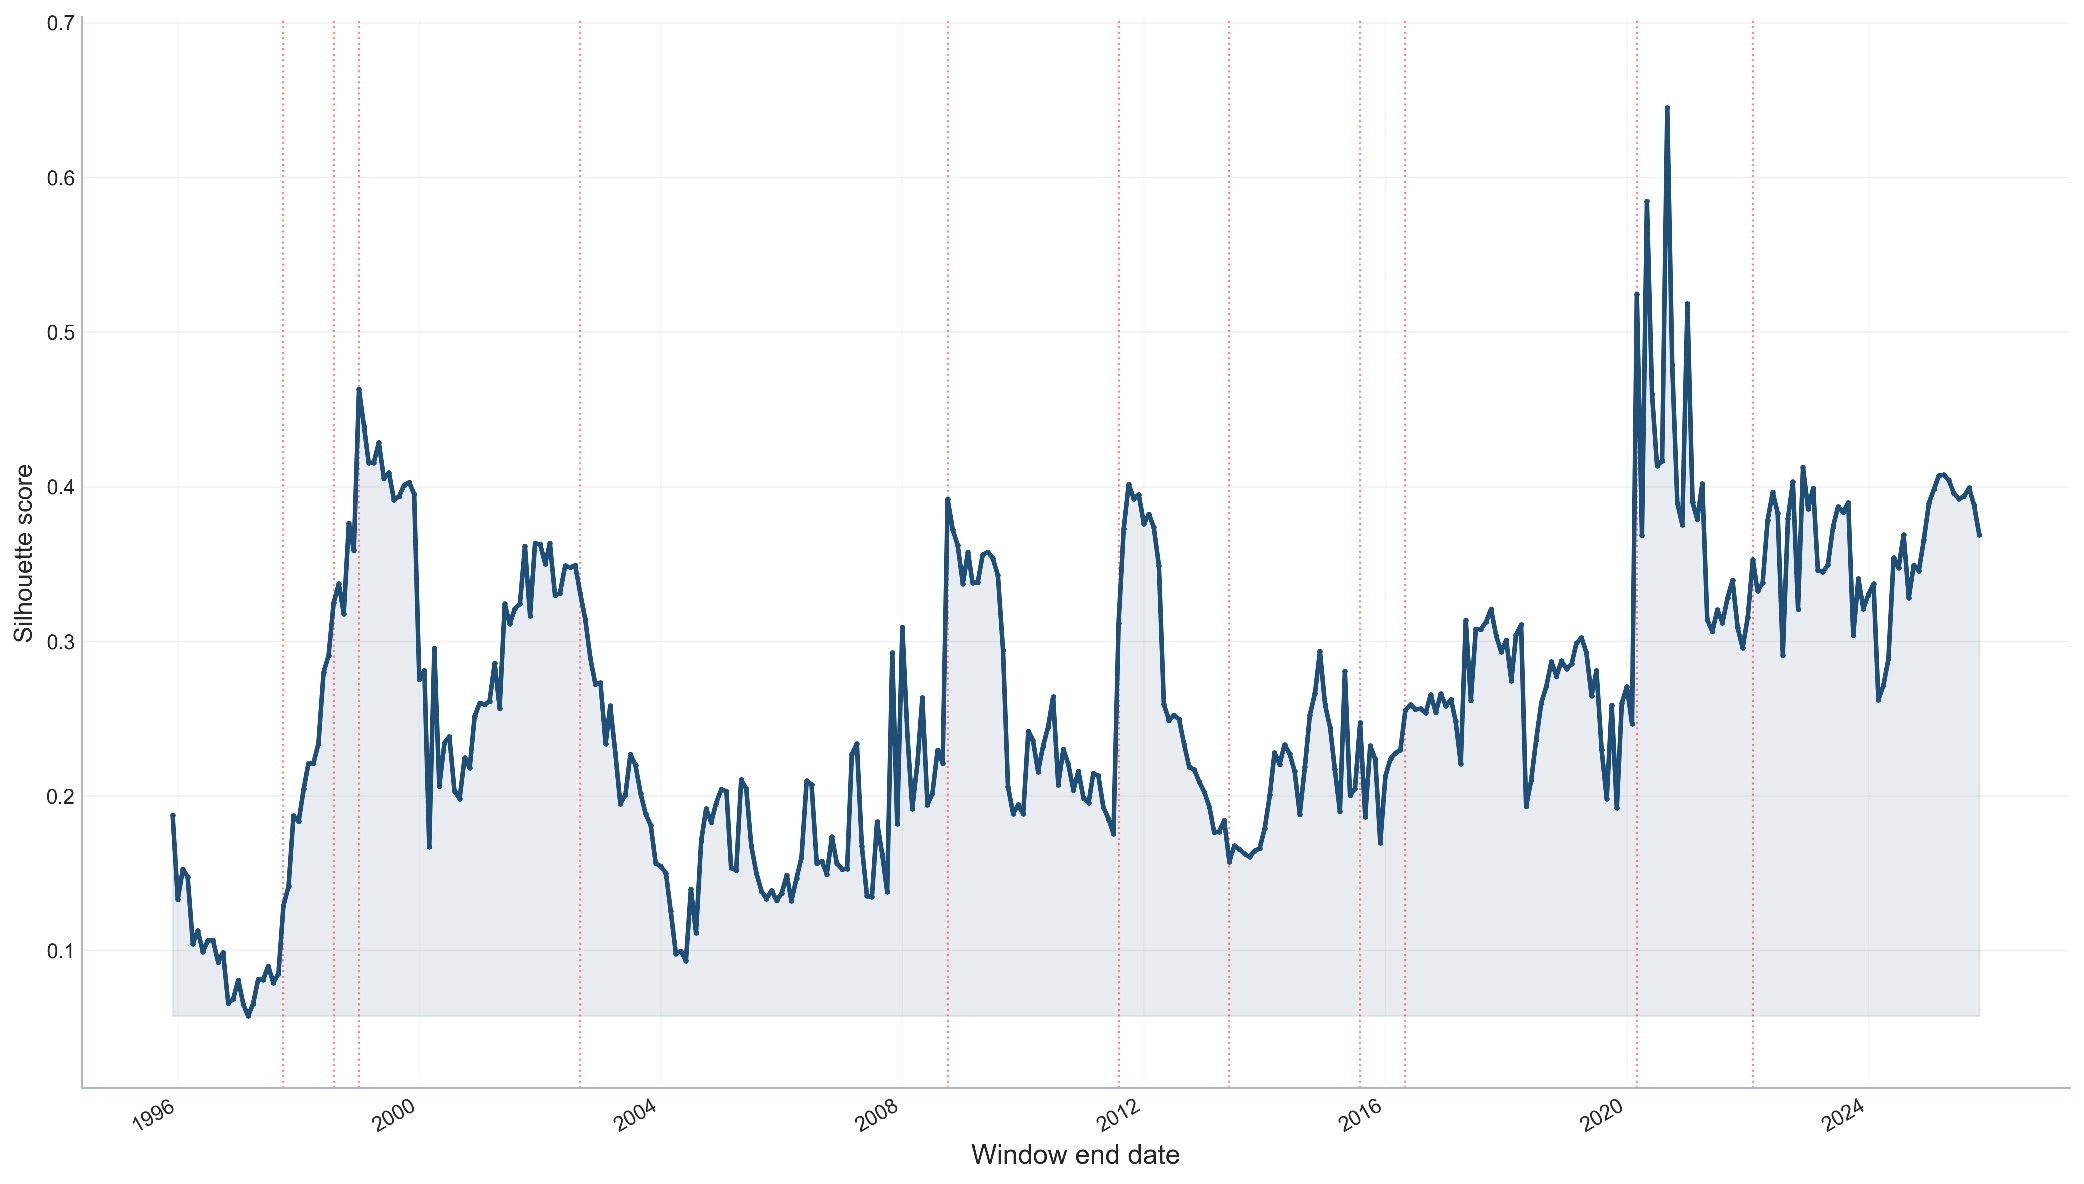
\includegraphics[width=\linewidth,keepaspectratio]{figures/validation/silhouette_evolucao.pdf}
\caption[Ward silhouette diagnostic]{Rolling silhouette score for Ward cluster cardinality across windows.}
\label{fig:cluster-validation-sil}
\end{center}

\begin{center}
\captionsetup{type=figure}
\centering
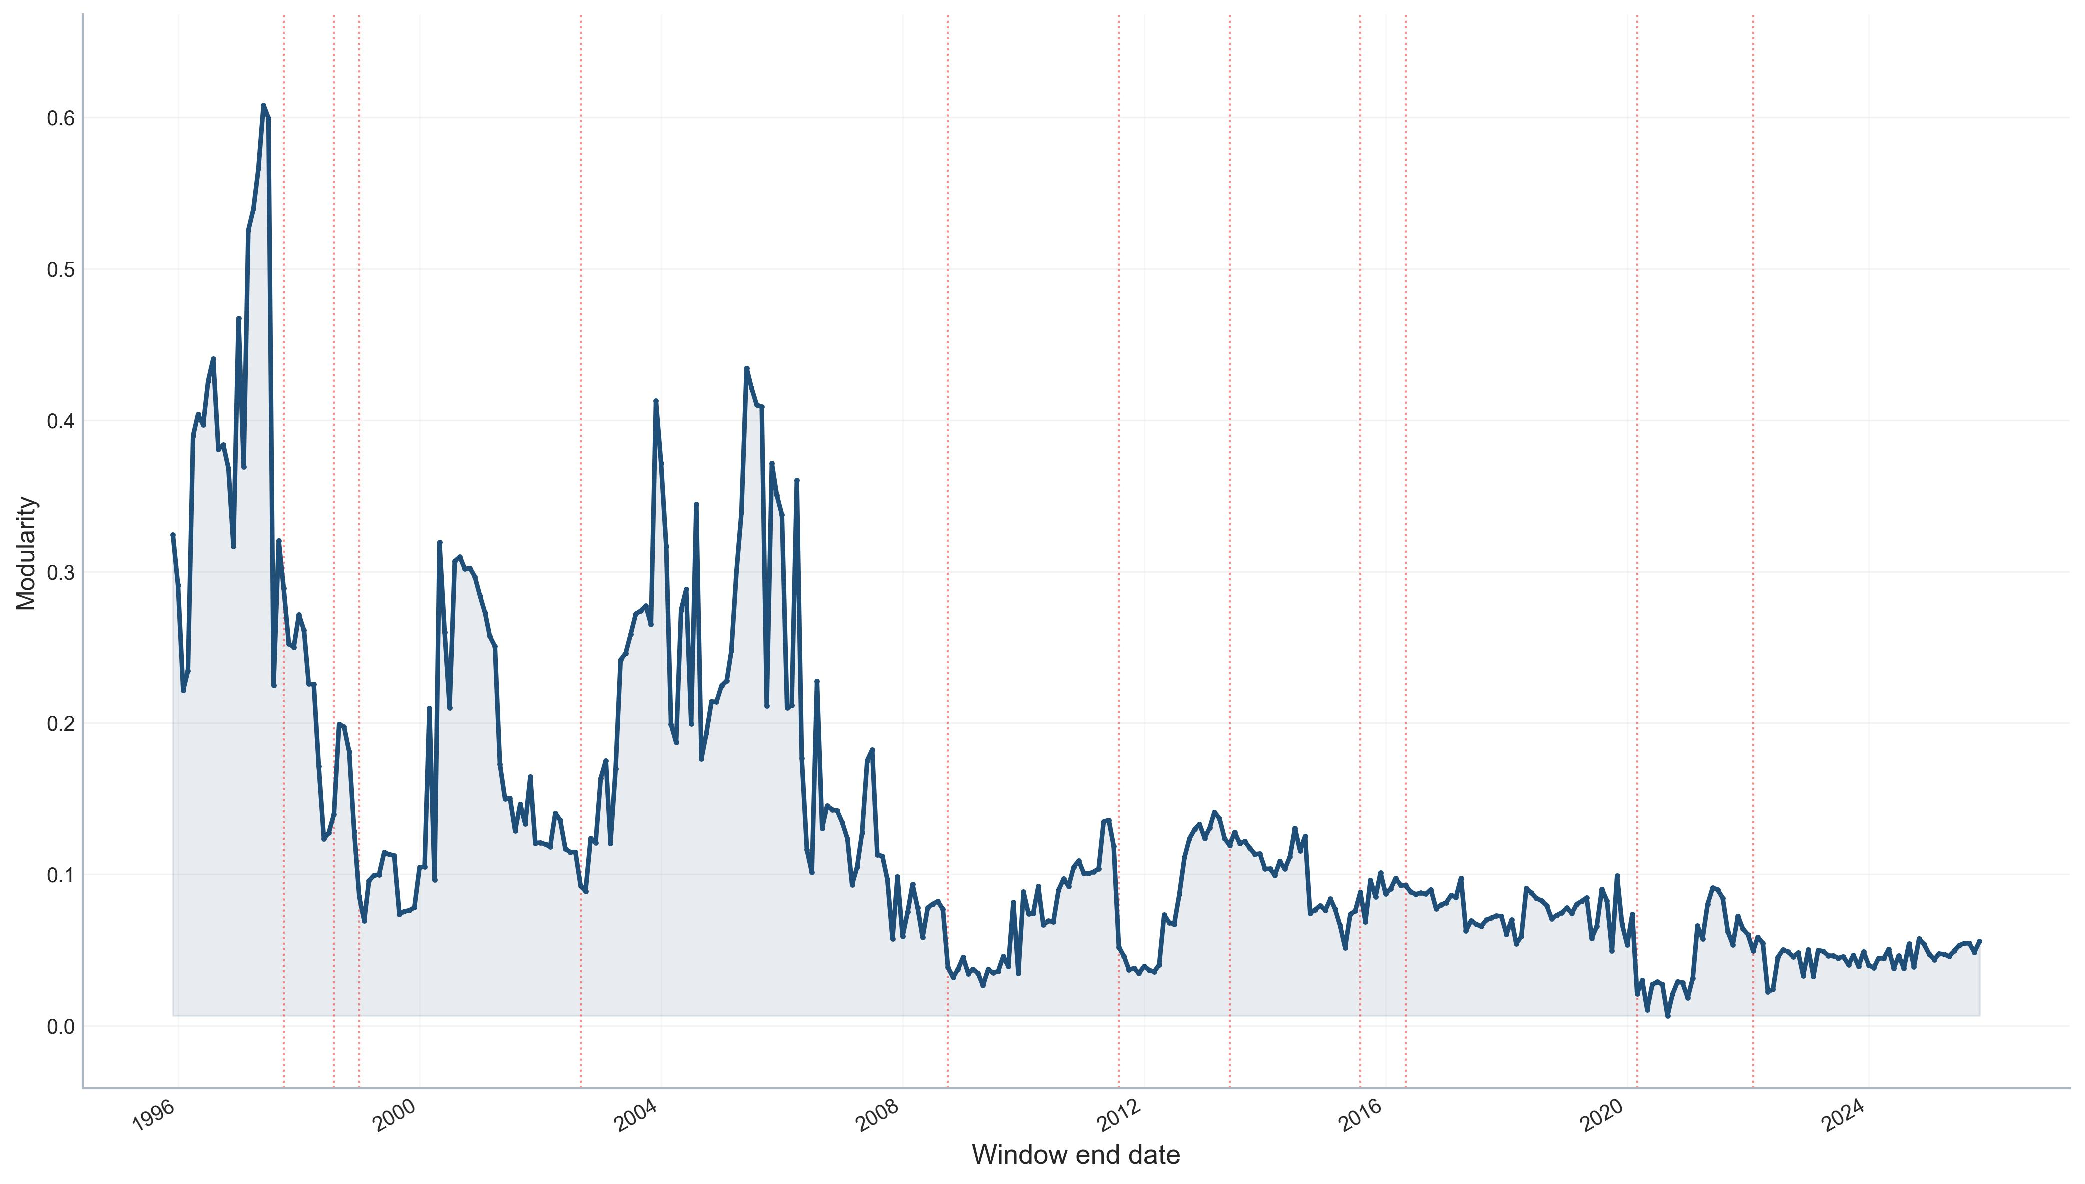
\includegraphics[width=\linewidth,keepaspectratio]{figures/validation/modularidade_evolucao.pdf}
\caption[Ward clustering modularity]{Rolling clustering modularity for the selected hierarchical configuration. The curve provides validation context for the Ward group residuals rather than a stand-alone crisis marker.}
\label{fig:cluster-validation-b}
\end{center}

This validation block connects directly to the multi-metric regime taxonomy used later in the paper. In all four configured crashes, KS displacement, MP signal variance, and the market-mode fraction are higher in event-containing windows than in the six local pre-event windows, each of which is a 12-month rolling sample ending before the shock day; post-event market-mode changes are positive in three of four cases. KS and MP therefore complement rather than replace the planar diagnostics: together they describe the correlation-matrix structure while communities, distances, modularity, and centralities identify mesoscopic configurations.

The first empirical message is that the rolling objects are stable enough to support interpretation. Across the 360-window history, the mean KS statistic is 0.6026, the mean KS $p$-value is near zero (0.00017), and 99.68\% of windows are stationary; the corresponding Ward diagnostics have mean best-$k$ equal to 2.36, mean silhouette equal to 0.262, and mean modularity equal to 0.133. The complete numerical summary is provided in Appendix~C, Table~\ref{tab:validation-summary}, so that the main text can reserve space for the substantive rolling and event comparisons. These aggregates show that the pipeline is not merely producing arbitrary pictures: it is persistently identifying non-random dependence structures and cluster partitions across the full 360-window history.

Moreover, the dynamic validation curves are supporting diagnostics rather than independent crisis results. Figure~\ref{fig:cluster-validation-sil} shows the rolling silhouette trajectory and Figure~\ref{fig:cluster-validation-b} the corresponding clustering modularity. They document measurement continuity, whereas the best-$k$ trajectory is retained in Appendix~C. Under Equation~\ref{eq:size_only_null}, these quantities remain conditional on the changing eligible universe and are not interpreted as independent crisis indicators.

The method-comparison sample reinforces why Ward linkage remains the preferred clustering lens. In representative windows, Ward often identifies richer partitions and higher modularity than average or complete linkage, especially in periods when the market still preserves internal segmentation. The representative comparisons are retained in Appendix~C, Table~\ref{tab:method-comparison}; the main text uses the resulting Ward partitions and their rolling quality diagnostics in the subsequent analyses.

\subsection{Heatmaps and Dendrograms: How Groups Form and Dissolve}

The hierarchical layer is retained as supplementary visual context for the central results. The heatmaps and dendrograms in Appendix~A (Figures~\ref{fig:heatmaps} and \ref{fig:dendrograms}) show whether correlation mass is concentrated inside identifiable blocks and how many meaningful branches the market supports at the beginning and end of the sample. Their interpretation remains descriptive and is complemented by the rolling community, distance, spectral, and clustering diagnostics reported below.

The full distance distribution is shown in Figure~\ref{fig:distance-kde-3d}. Its three-dimensional KDE surface is a complex distributional diagnostic, so it is placed immediately after this overview and before the remaining contextual discussion.

\begin{center}
\captionsetup{type=figure}
\centering
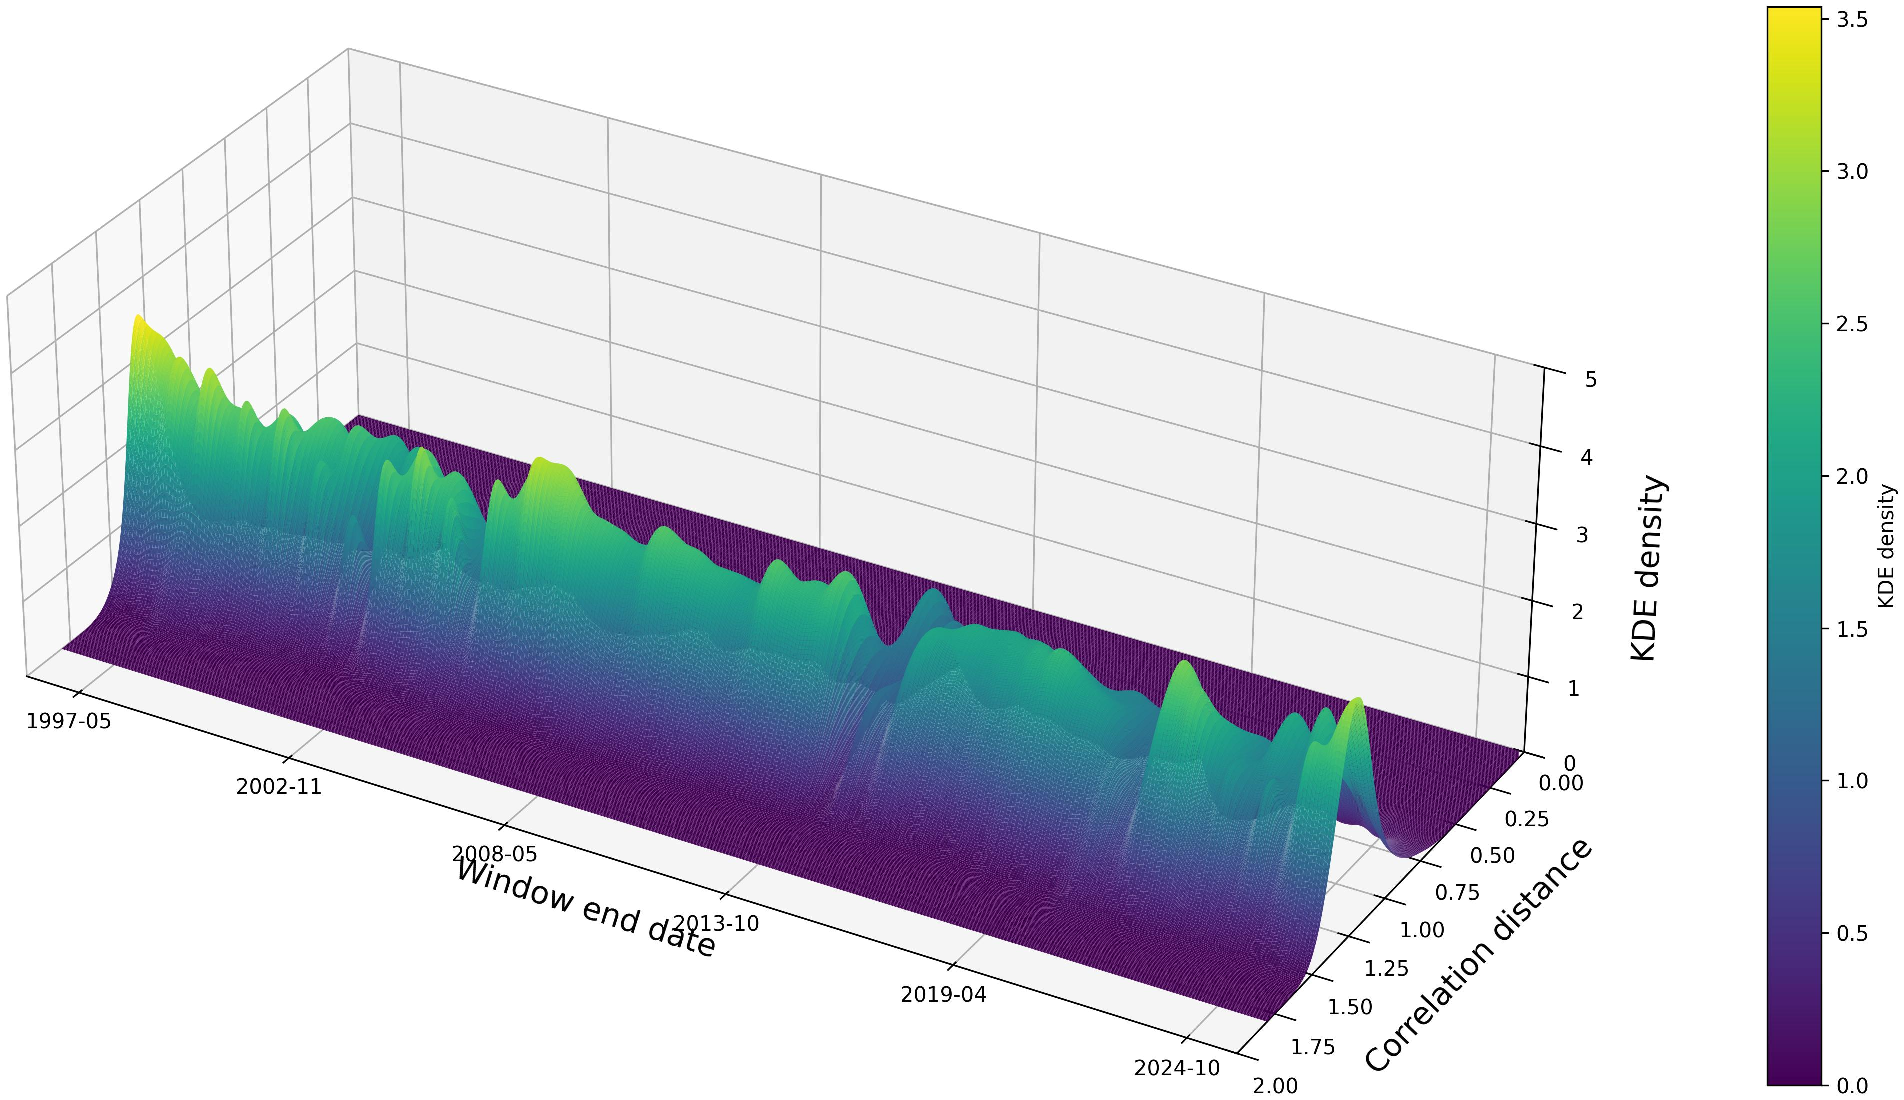
\includegraphics[width=\linewidth,keepaspectratio]{figures/statistics/cdf3d_distancia_Planar.pdf}
\caption{Three-dimensional rolling KDE of PMFG edge distances across windows. The surface stacks separately normalized window-level kernel densities and provides distributional context for changes in mean, dispersion, skewness, and kurtosis. The event comparison identifies distance compression as an important but episode-specific component of reconfiguration; the surface is not interpreted as a universal crisis trajectory.}
\label{fig:distance-kde-3d}
\end{center}

The KDE surface should be read in two directions. Movement along the horizontal
window axis records the evolution of the market, whereas movement along the
distance axis records how the retained PMFG edges are redistributed. A ridge
that moves toward shorter distances is consistent with geometric compression;
changes in ridge width indicate redistribution of separation rather than a
simple level shift. The surface therefore supplies a visual check on the
four-moment summary, while the event tables remain the basis for comparing
configured phases.

Because each window-level density is normalized separately, the vertical scale
should not be interpreted as a market-wide volume or probability level across
dates. The relevant evidence is the changing location and shape of the density
within each window and its agreement with the mean, variance, skewness, and
kurtosis results. This preserves the descriptive scope of the KDE and avoids
turning a complex visualization into a standalone crisis classifier.

The corresponding numerical interpretation is supplied by the rolling community, distance, spectral, and clustering metrics; the two boundary-window figures are provided in Appendix~A as visual context for the rolling KDE and planar trajectories.

These figures provide descriptive context for portfolio construction and stress-period comparison. When heatmap blocks are well separated, diversification by correlation group is more plausible. When the matrix thickens off the diagonal and the dendrogram contracts into fewer dominant branches, portfolios that seemed diversified under sector labels may become structurally more homogeneous.

\begin{center}
\captionsetup{type=figure}
\centering
\begin{subfigure}{0.99\linewidth}
    \centering
    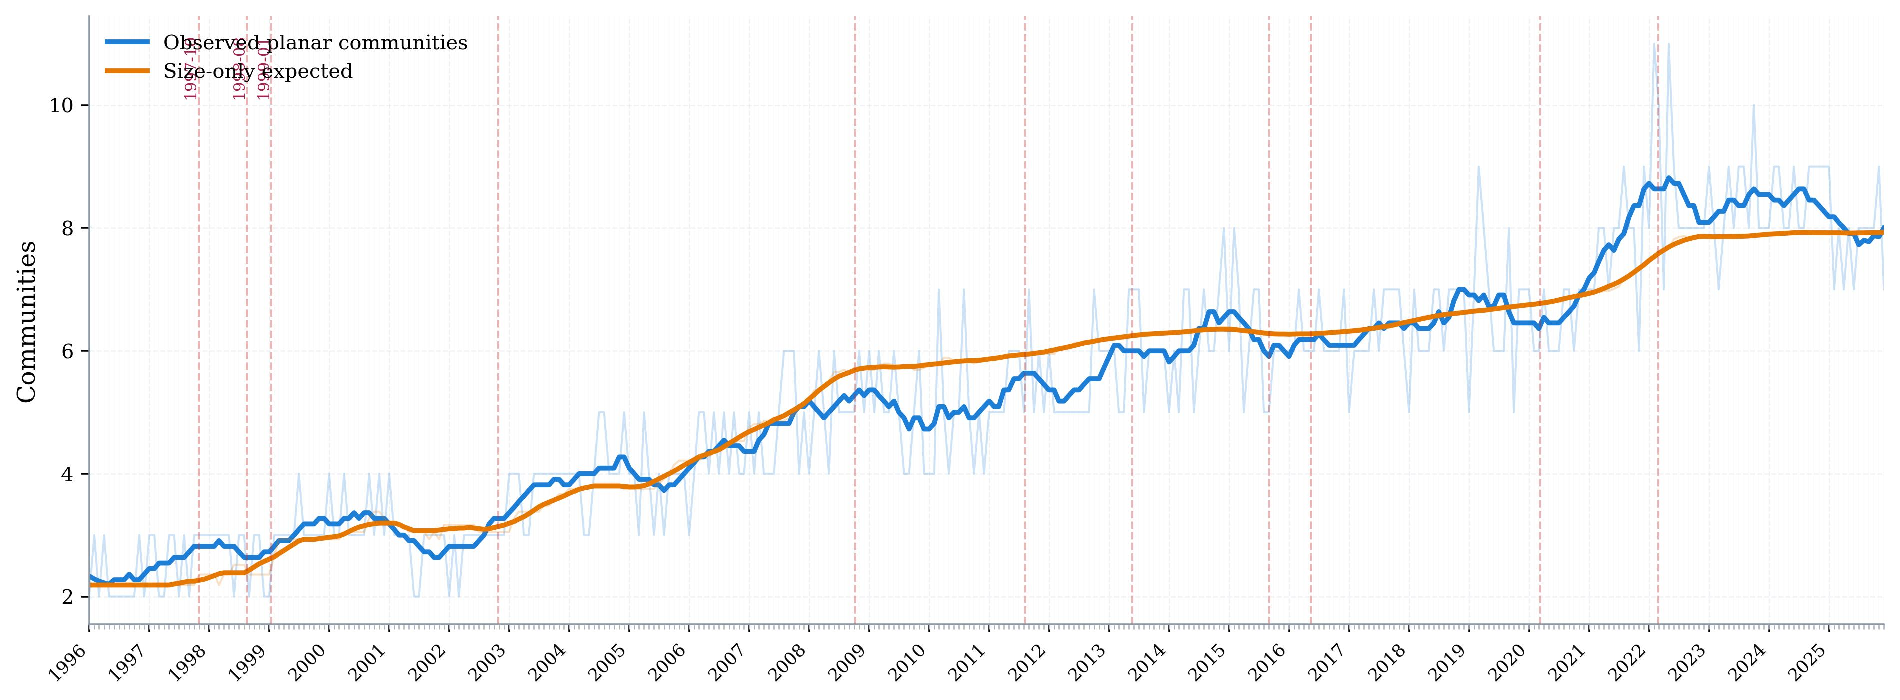
\includegraphics[width=\linewidth,keepaspectratio]{figures/validation/groups_fig10a_planar_communities_paper.pdf}
    \caption{Rolling planar (PMFG) community evolution across 360 windows.}
    \label{fig:groups-10a}
\end{subfigure}
\vspace{0.5em}
\begin{subfigure}{0.99\linewidth}
    \centering
    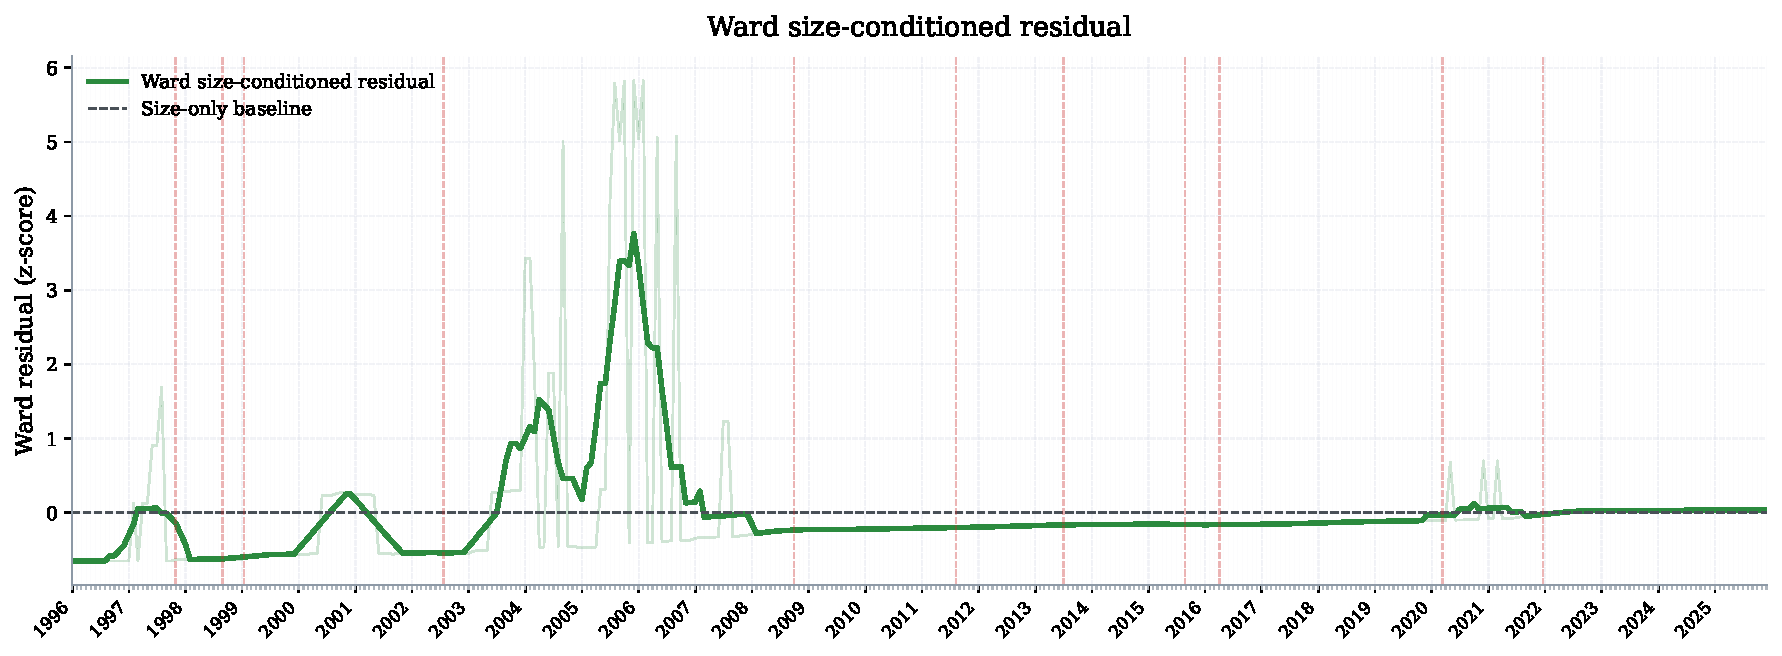
\includegraphics[width=\linewidth,keepaspectratio]{figures/validation/groups_fig10b_ward_timeseries_paper.pdf}
    \caption{Ward size-conditioned residual across the 360 rolling windows. The residual is the observed Ward partition relative to the full-panel size-only baseline, expressed as a z-score; negative values indicate hierarchical compression beyond the mechanical effect of the changing eligible universe. Red vertical lines mark the eleven sensitivity anchors without date labels.}
    \label{fig:groups-10b}
\end{subfigure}
\caption[Planar topology and Ward residual trajectory]{(a) Raw rolling PMFG community count across the 360 windows, providing descriptive context for changes in planar grouping. (b) Ward size-conditioned residual trajectory. Negative values indicate fewer Ward groups than expected after controlling for the changing eligible universe. Red vertical lines mark the eleven sensitivity anchors without date labels.}
\label{fig:groups-validation-pair}
\end{center}

\subsection{Planar-Only Structural Evidence}

Given the scope of this study, the results section prioritizes planar-network evidence only. Complete-graph and significance-filtered temporal diagnostics are intentionally omitted from the core interpretation. The substantive financial interpretation remains anchored in the planar representation throughout.

\subsection{Planar Topology and the Four Crisis Moments}

The central empirical result of the paper is that systemic stress in B3 is associated with a reconfiguration of mesoscale topology rather than with a uniform movement in every diagnostic. Figures~\ref{fig:planar-groups} and \ref{fig:planar-communities} provide rolling context through modularity and the number of planar communities, while the size-adjusted pooled comparison is retained in Appendix~C (Figure~\ref{fig:groups-residuals}) as supporting evidence. The raw trajectories are not used as event evidence because they do not distinguish tranquil, pre-event, event-containing, and post-event phases.

Under Equation~\ref{eq:size_only_null}, the relevant question is not whether later windows contain more firms, but whether observed communities exceed or fall short of the amount mechanically implied by the larger universe. The pooled crisis comparison shows modest planar-community contraction and a sharper Ward-group residual shift; it does not establish that every event or every phase follows the same pattern.

The raw modularity and community-count trajectories provide useful background and establish the rolling mesoscopic context. Figures~\ref{fig:planar-groups} and \ref{fig:planar-communities} show these two raw trajectories; the size-conditioned residual comparison below is the relevant cross-window diagnostic.

\begin{center}
\captionsetup{type=figure}
\centering
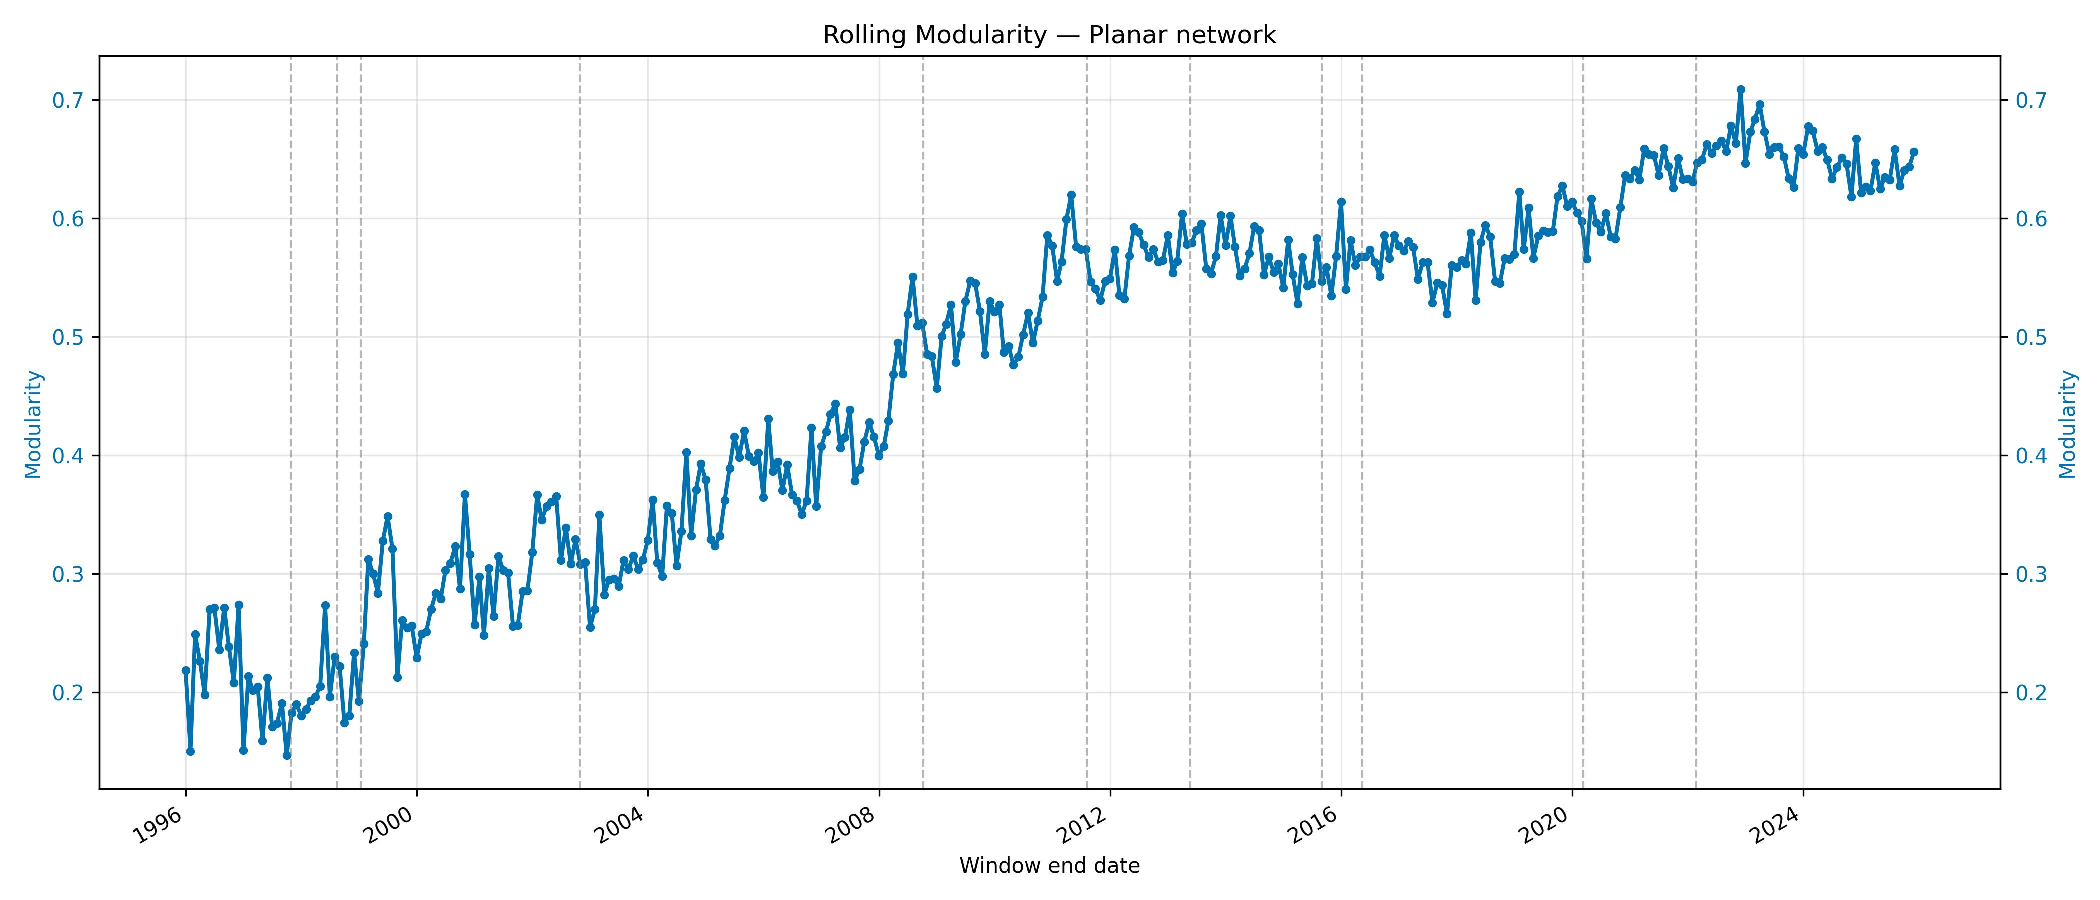
\includegraphics[width=\paperfigwidth]{figures/networks/Planar_modularidade_evolucao.pdf}
\caption{Rolling planar modularity across all 360 windows. The planar network is the main structural lens of the paper because it preserves mesoscopic organization while remaining sparse enough to interpret.}
\label{fig:planar-groups}
\end{center}

\begin{center}
\captionsetup{type=figure}
\centering
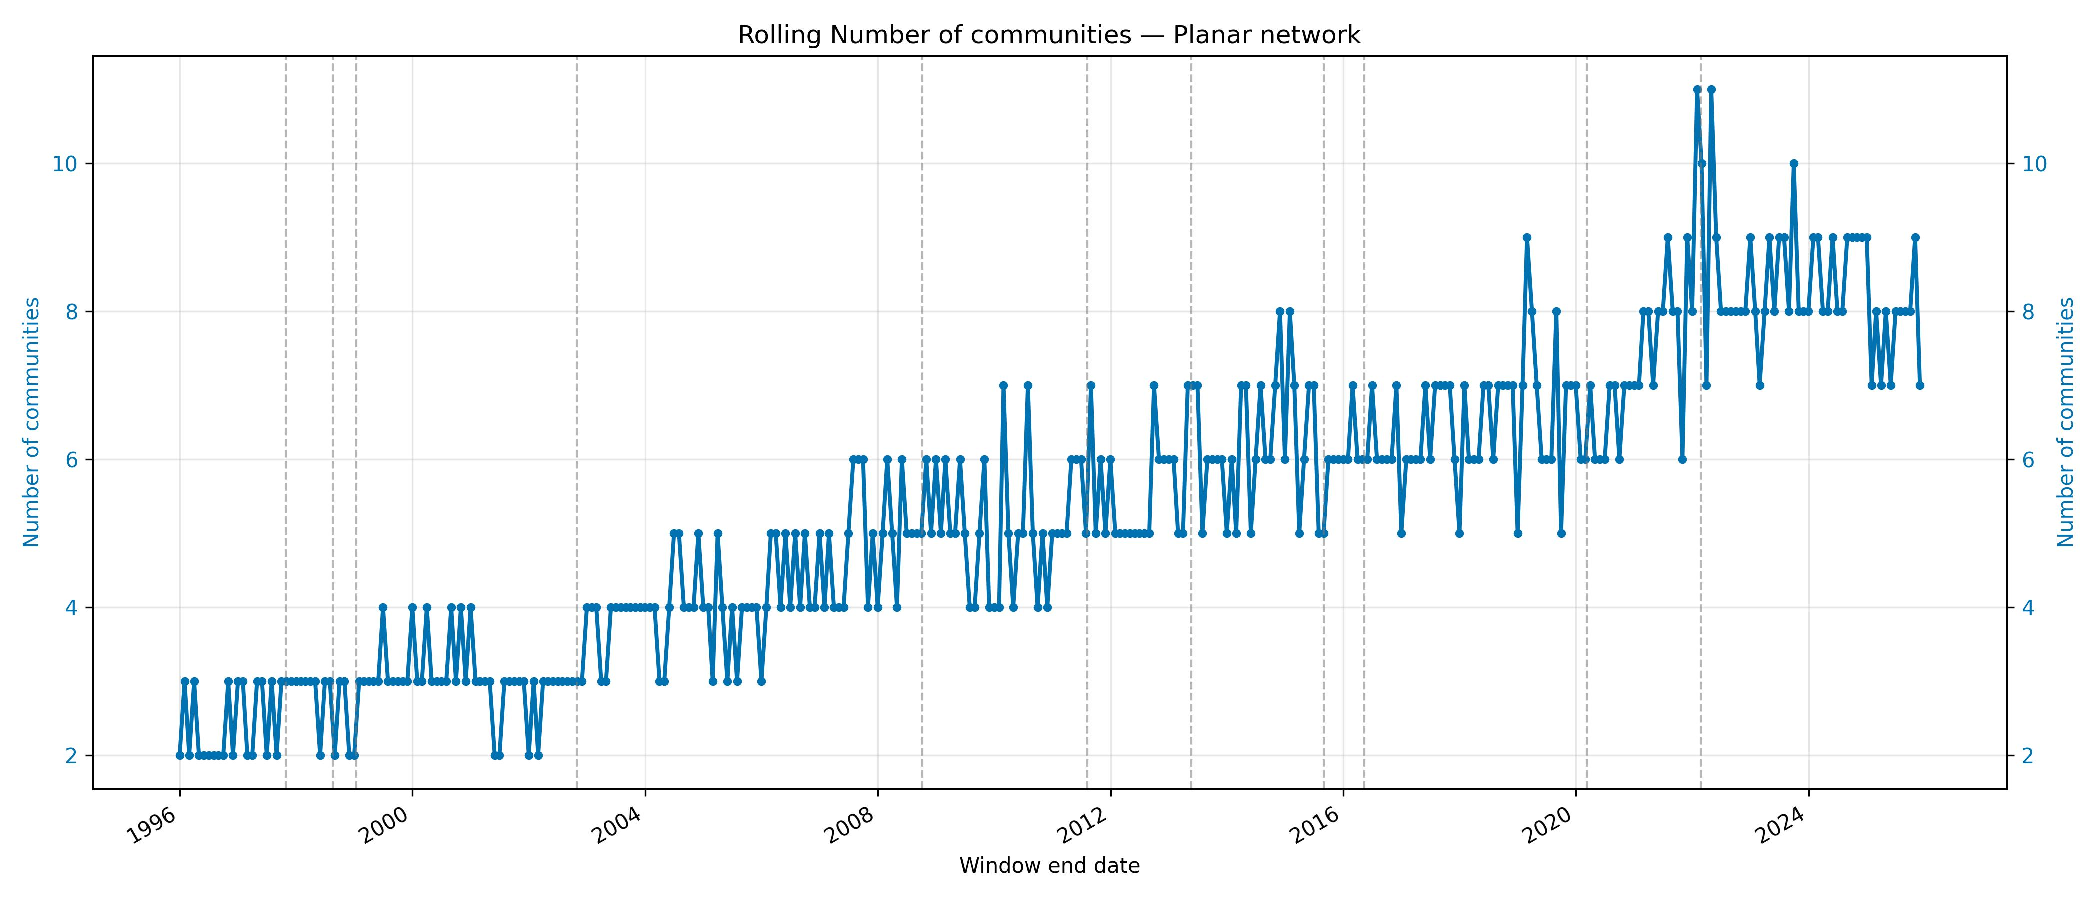
\includegraphics[width=\paperfigwidth]{figures/networks/Planar_num_communities_evolucao.pdf}
\caption{Raw rolling number of planar communities across the 360 windows. Variations provide descriptive context for planar grouping and are interpreted jointly with the size-adjusted community residuals rather than as a stand-alone crisis signature.}
\label{fig:planar-communities}
\end{center}

The residual boxplots provide the pooled size-conditioned comparison. The negative Ward shift is sharper than the planar-community shift, while the spread of both distributions shows why the pooled result cannot replace event-by-event phase analysis. In practical terms, the figure identifies a difference in aggregate organization after the size control, not a universal response for every anchor.

The pooled size-adjusted comparisons provide limited context only. Crisis windows do not contain more planar nodes on average; they contain slightly fewer, with 67.97 nodes in crisis against 70.07 outside crisis. Once Equation~\ref{eq:size_only_null} is applied, planar community compression remains present but modest: the mean residual is $-0.0176$ in crisis windows and $0.0087$ outside crisis. The same exercise on the hierarchical Ward family is sharper, with mean residual $-0.2942$ in crises versus $0.1453$ outside crises. These two-regime aggregates are not treated as evidence for a common event sequence; the four-phase interpretation is reserved for the event-level comparisons below.

The continuous planar metrics tell an even clearer story. Mean PMFG distance falls from 1.1616 outside crisis to 1.0887 in crisis windows, and after Equation~\ref{eq:size_only_topology_null} the corresponding residual remains strongly negative in crisis ($-0.0489$) and positive outside crisis ($0.0241$). Distance variance moves in the opposite direction: its residual is $0.0037$ in crisis and $-0.0018$ outside crisis, indicating that compression is accompanied by a redistribution of cross-sectional separation rather than a uniform collapse of all edges to the same level. Modularity behaves differently: the observed planar modularity is slightly higher in crisis (0.4728) than outside crisis (0.4684), and the adjusted residual is mildly positive in crisis (0.0032). This is substantively important. In the PMFG, crises do not look like complete topological disintegration; they look like shorter effective distances and tighter system-wide coupling coexisting with persistent local organization. For diversification, this is the more adverse scenario: the market remains structured, but that structure becomes more compressed and therefore less useful for isolating independent risk blocks.

The pooled comparisons summarize windows associated with the configured stress dates; they do not substitute for an event-by-event test. For the four configured dates, the centrality phase table records six-month pre-event and post-event summaries and rolling windows containing each date. Its signs vary across events, so it is used to describe heterogeneous configurations rather than to assert a universal crisis sequence.

This evidence motivates the following descriptive reading of the rolling configurations:
\begin{enumerate}
    \item \textbf{Tranquil windows}: more groups, larger average distances, and structurally credible diversification across correlation blocks.
    \item \textbf{Pre-event windows}: possible deviations in group structure, distance, and centrality relative to the size-conditioned reference.
    \item \textbf{Event-containing windows}: configurations that can include shorter financial distances and altered dispersion.
    \item \textbf{Post-event windows}: subsequent configurations that need not restore the preceding level or follow a common direction across events.
\end{enumerate}

The centrality plots refine this descriptive interpretation after removing their size-only expectations. Mean degree is excluded from the figure because maximal planarity fixes it exactly at $6-12/N_t$, making its residual identically zero and unsuitable as a regime diagnostic. The betweenness, eigenvector, and closeness panels show residual mean centralities, namely observed values minus the expectation conditional on $\log(1+N_t)$. They consequently describe changes in brokerage, core placement, and reachability that remain after the changing universe is discounted, without attributing them to a causal crisis mechanism. Figures~\ref{fig:planar-betweenness}, \ref{fig:planar-eigenvector}, \ref{fig:planar-centralities-b}, and \ref{fig:planar-dist-mean}--\ref{fig:planar-dist-kurt} summarize these complementary aspects.

\begin{center}
\captionsetup{type=figure}
\centering
\begin{subfigure}{0.99\linewidth}
    \centering
    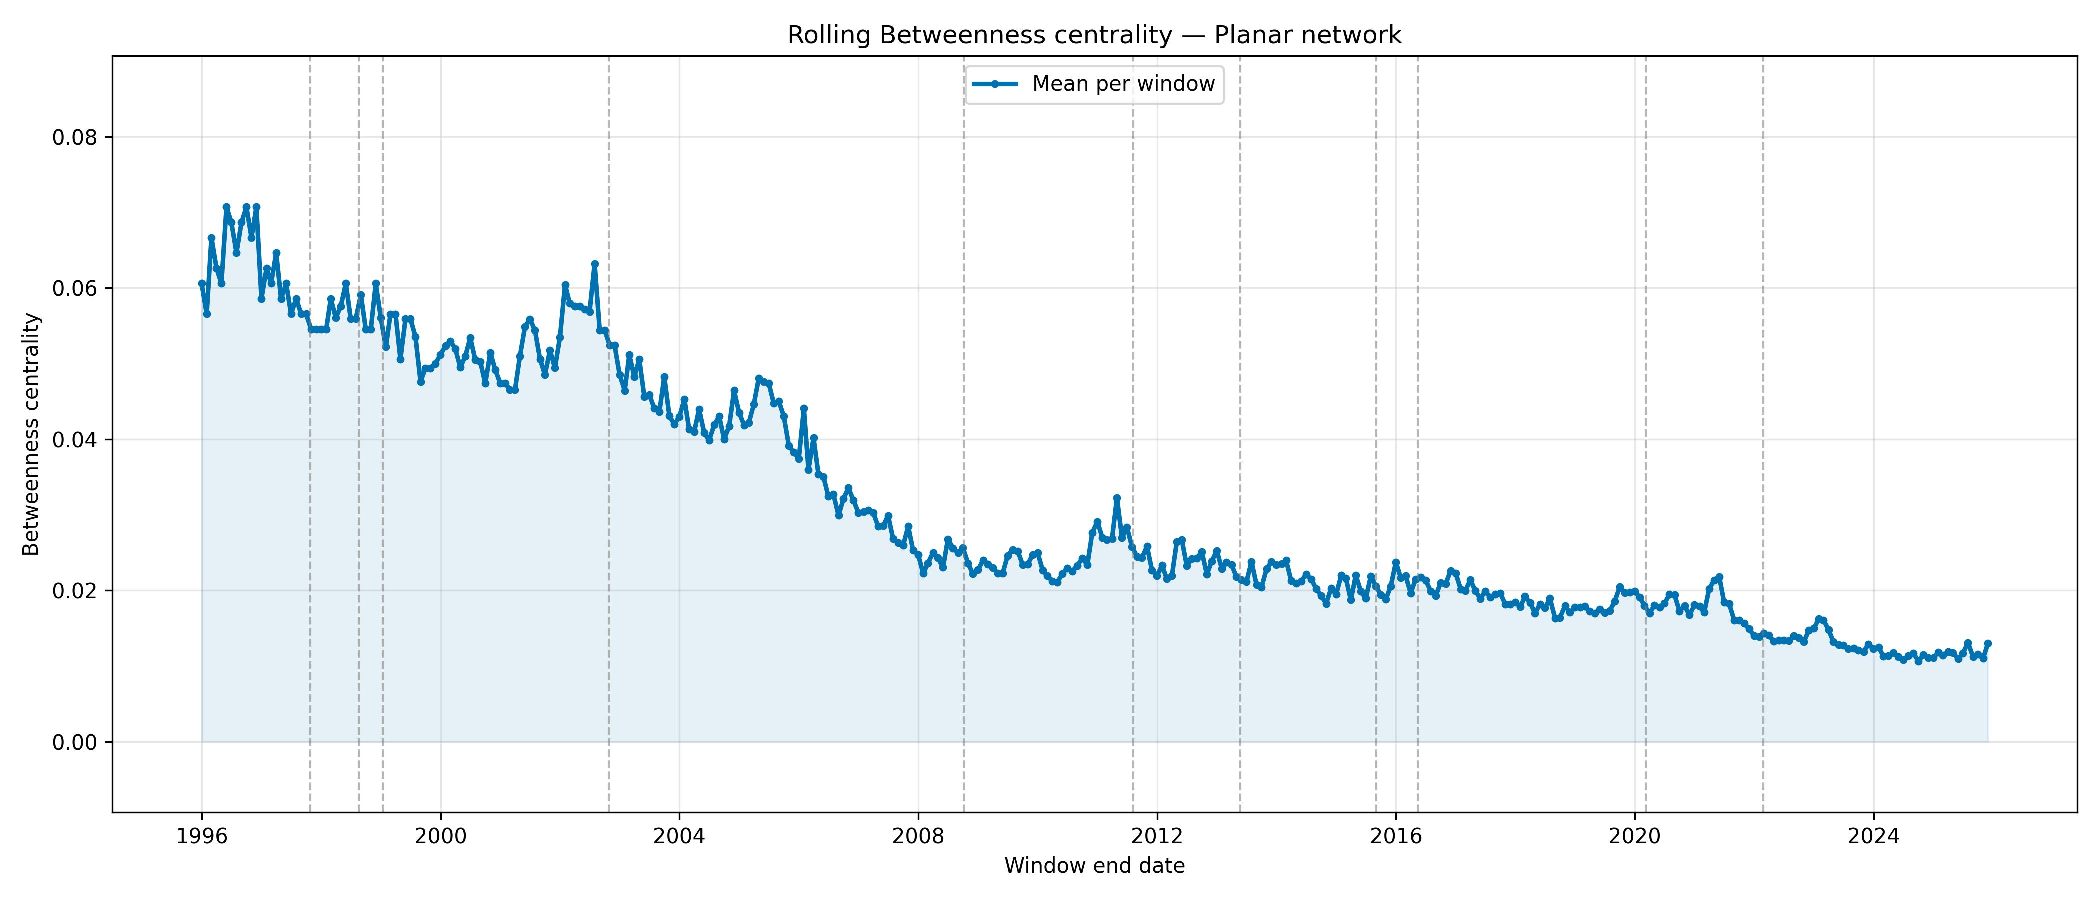
\includegraphics[width=\linewidth,keepaspectratio]{figures/networks/Planar_betweenness_centrality_evolucao.pdf}
    \caption{Mean betweenness residual.}
    \label{fig:planar-betweenness}
\end{subfigure}

\begin{subfigure}{0.99\linewidth}
    \centering
    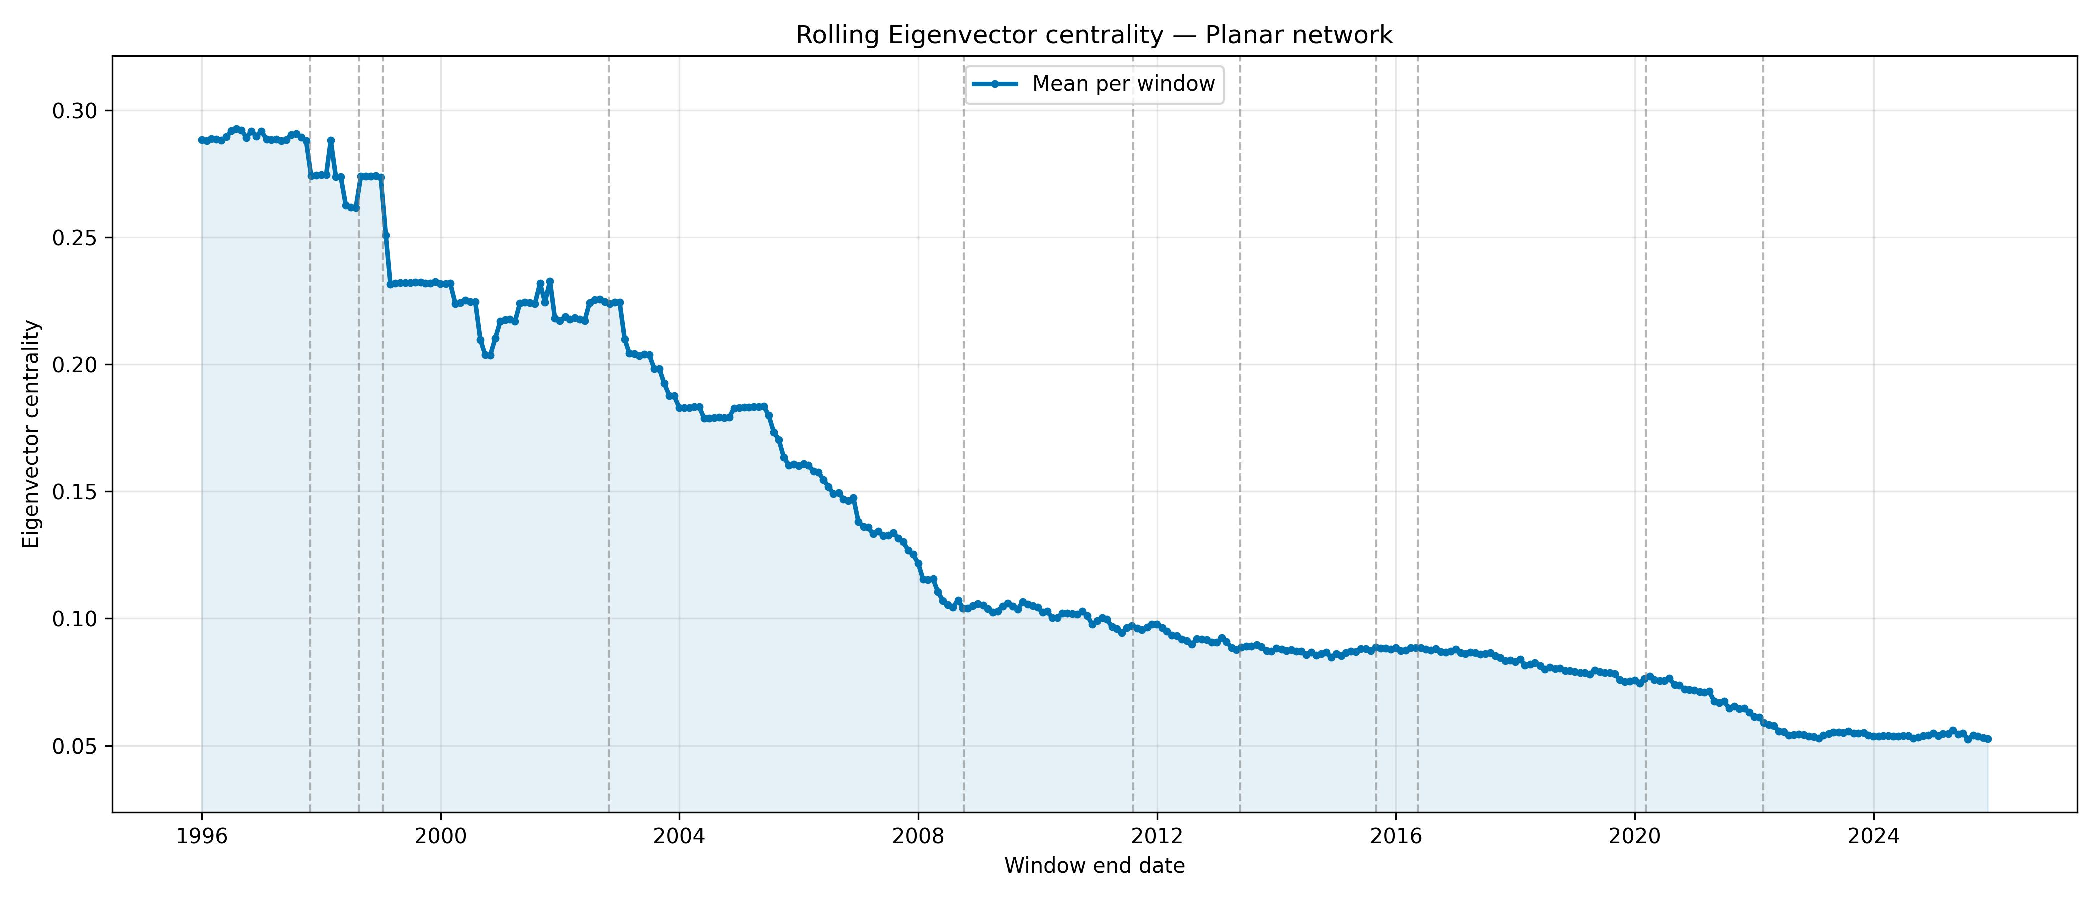
\includegraphics[width=\linewidth,keepaspectratio]{figures/networks/Planar_eigenvector_centrality_evolucao.pdf}
    \caption{Mean eigenvector-centrality residual.}
    \label{fig:planar-eigenvector}
\end{subfigure}

\caption{Size-adjusted rolling betweenness and eigenvector-centrality diagnostics. Each curve is observed mean centrality minus its size-conditioned expected value.}
\label{fig:planar-centralities-a}
\end{center}

The paired centrality panels show how the size-conditioned network position changes through time. Betweenness and eigenvector centrality capture complementary aspects of brokerage and core placement; neither should be read as a stand-alone stress signal. Their residual formulation is essential because the admissible B3 universe changes across the 30-year sample.

\begin{center}
\captionsetup{type=figure}
\centering
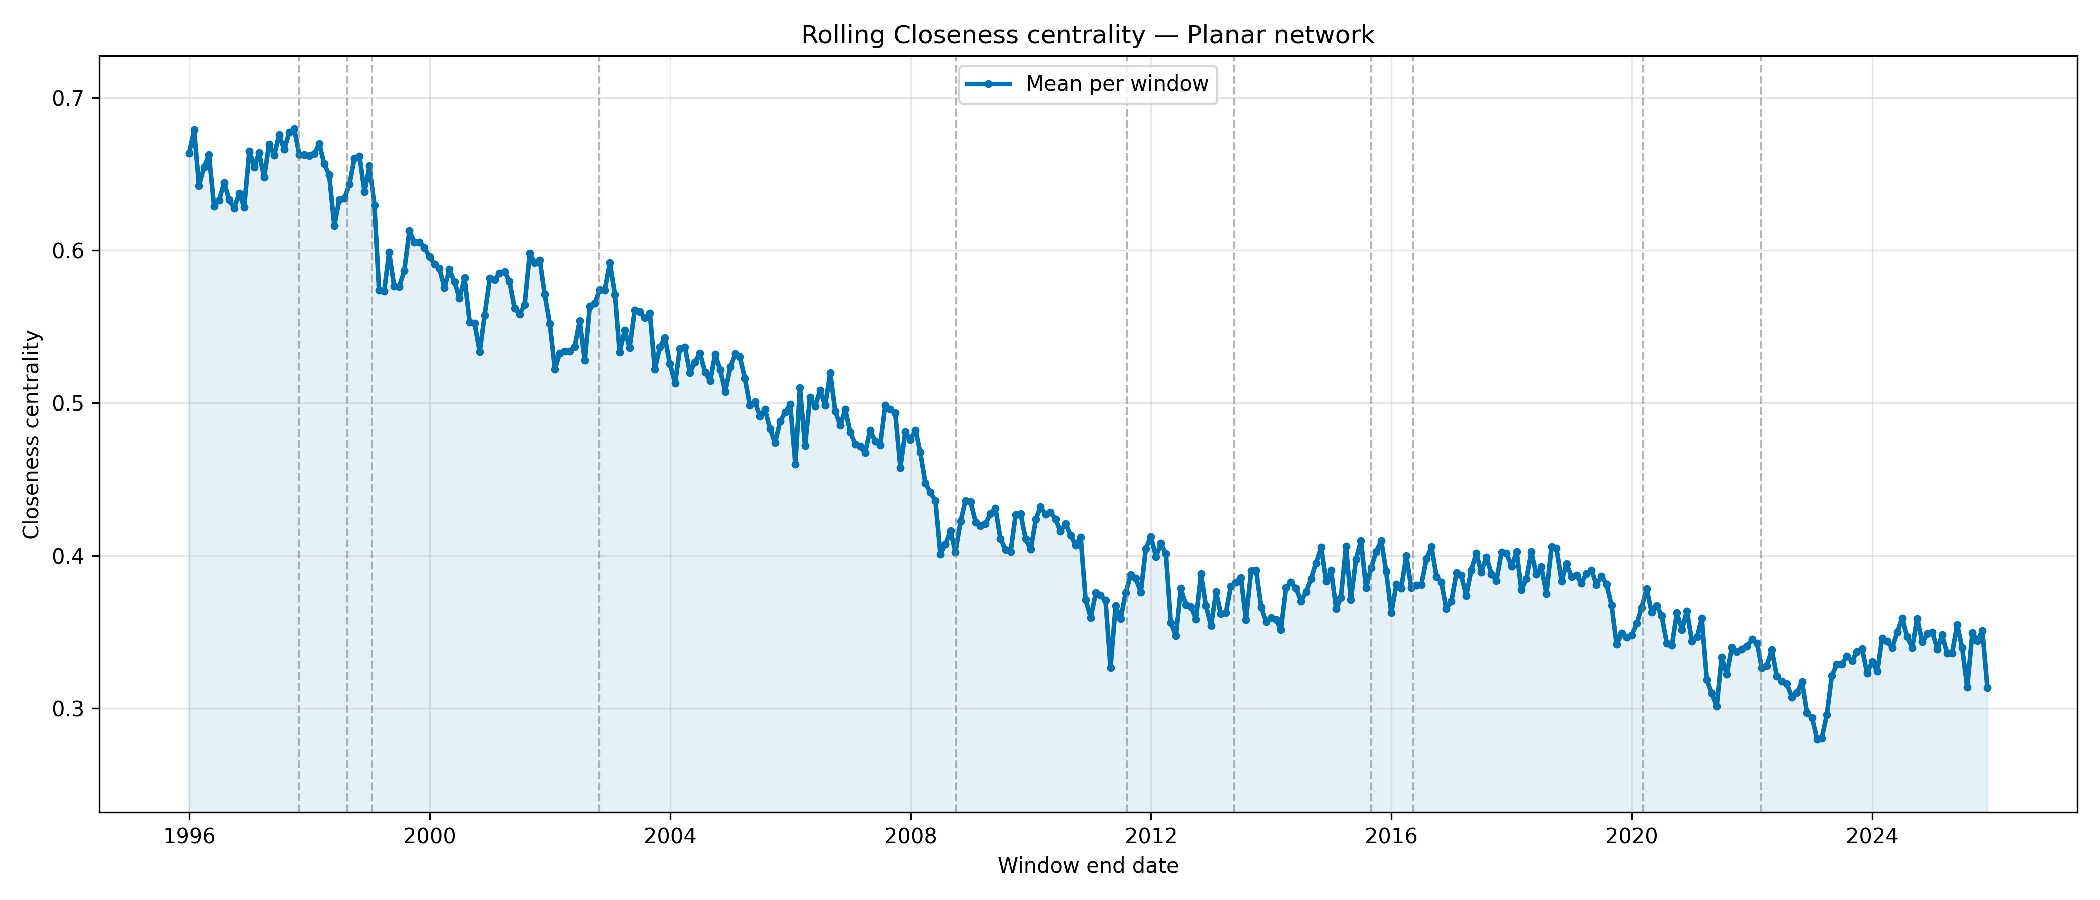
\includegraphics[width=\linewidth,keepaspectratio]{figures/networks/Planar_closeness_centrality_evolucao.pdf}
\caption{Size-adjusted rolling closeness-centrality diagnostic. The curve is observed mean centrality minus its size-conditioned expected value and describes reachability across the tranquil/pre-crisis/during/post-crisis taxonomy. Mean degree is omitted because its PMFG residual is identically zero under the exact maximal-planar identity $6-12/N$.}
\label{fig:planar-centralities-b}
\end{center}

The closeness panel completes the centrality block by describing residual reachability. Its interpretation is kept separate from the other two centralities because the three measures respond differently to the same topology. Together they document heterogeneous structural positioning rather than a common directional trajectory.

The four distribution moments complement the centrality evidence by separating average compression from changes in spread, asymmetry, and concentration. Figures~\ref{fig:planar-dist-mean}--\ref{fig:planar-dist-kurt} show that crises alter the full shape of the financial-distance distribution rather than only its mean.

\begin{center}
\captionsetup{type=figure}
\centering
\begin{subfigure}{0.99\linewidth}
    \centering
    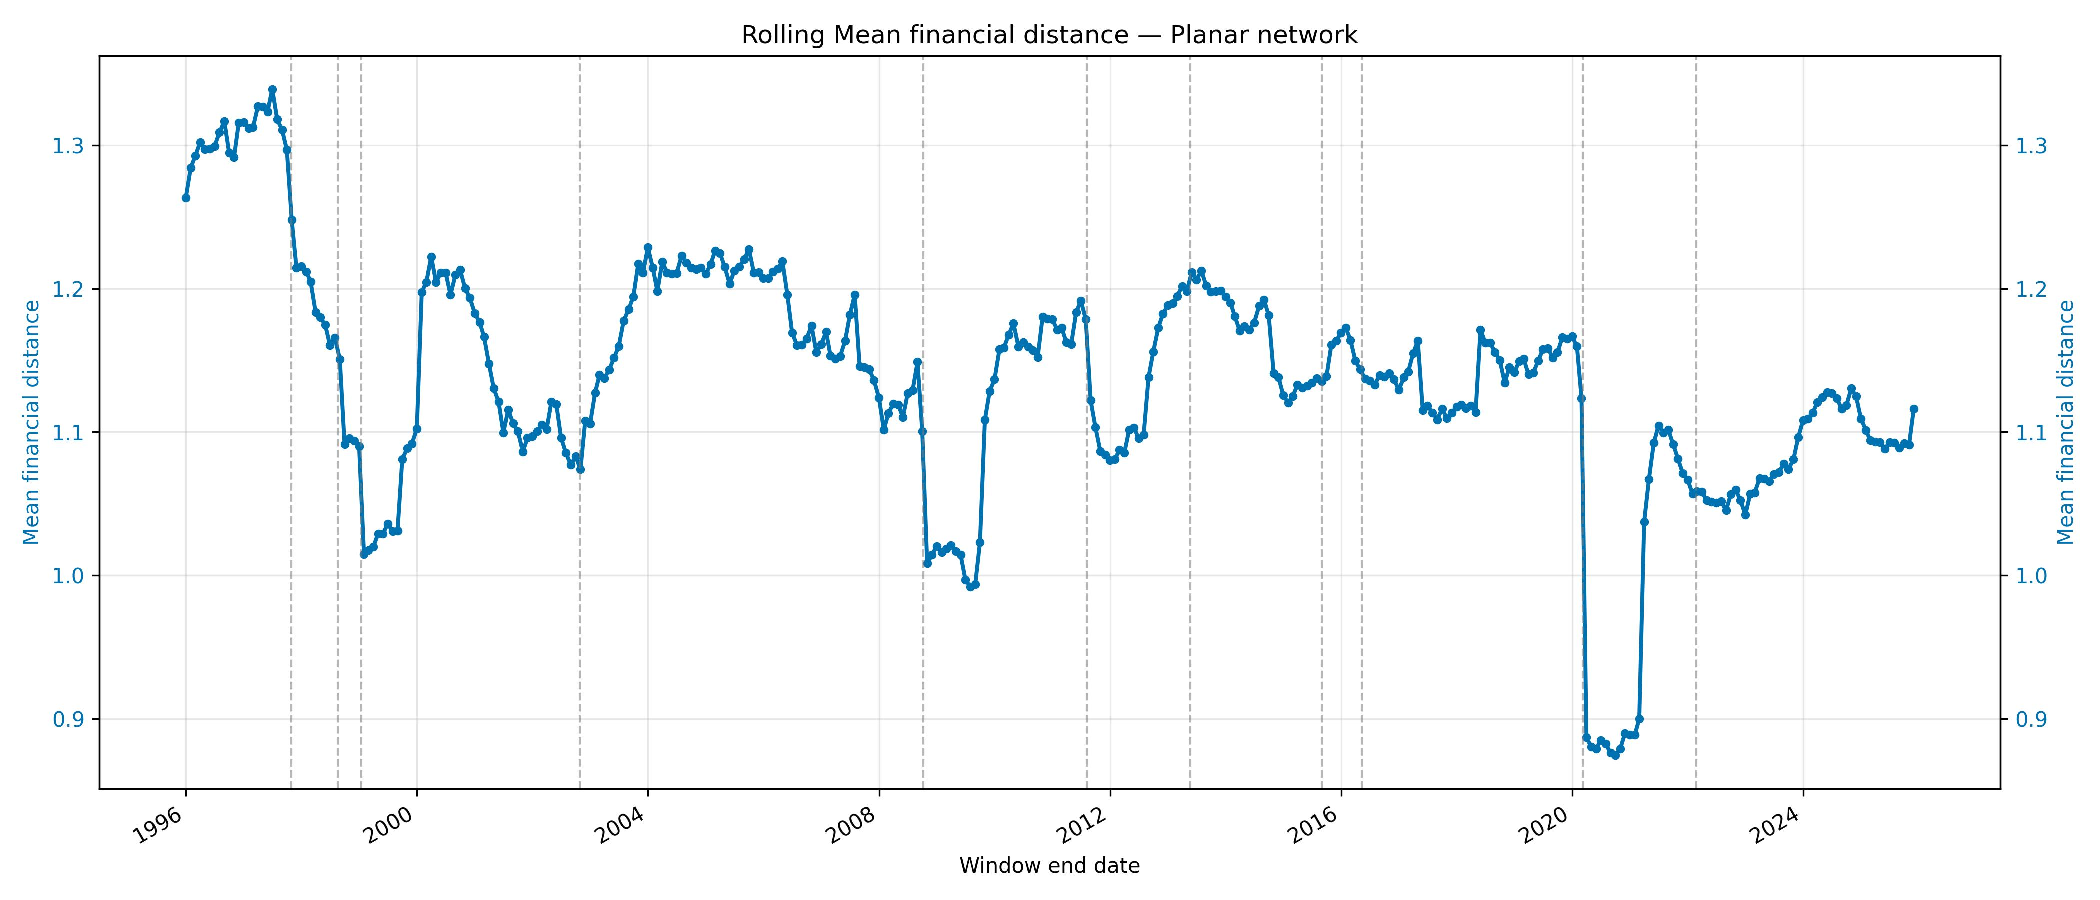
\includegraphics[width=\linewidth,keepaspectratio]{figures/networks/Planar_dist_mean_evolucao.pdf}
    \caption{Mean distance.}
    \label{fig:planar-dist-mean}
\end{subfigure}

\vspace{0.55em}

\begin{subfigure}{0.99\linewidth}
    \centering
    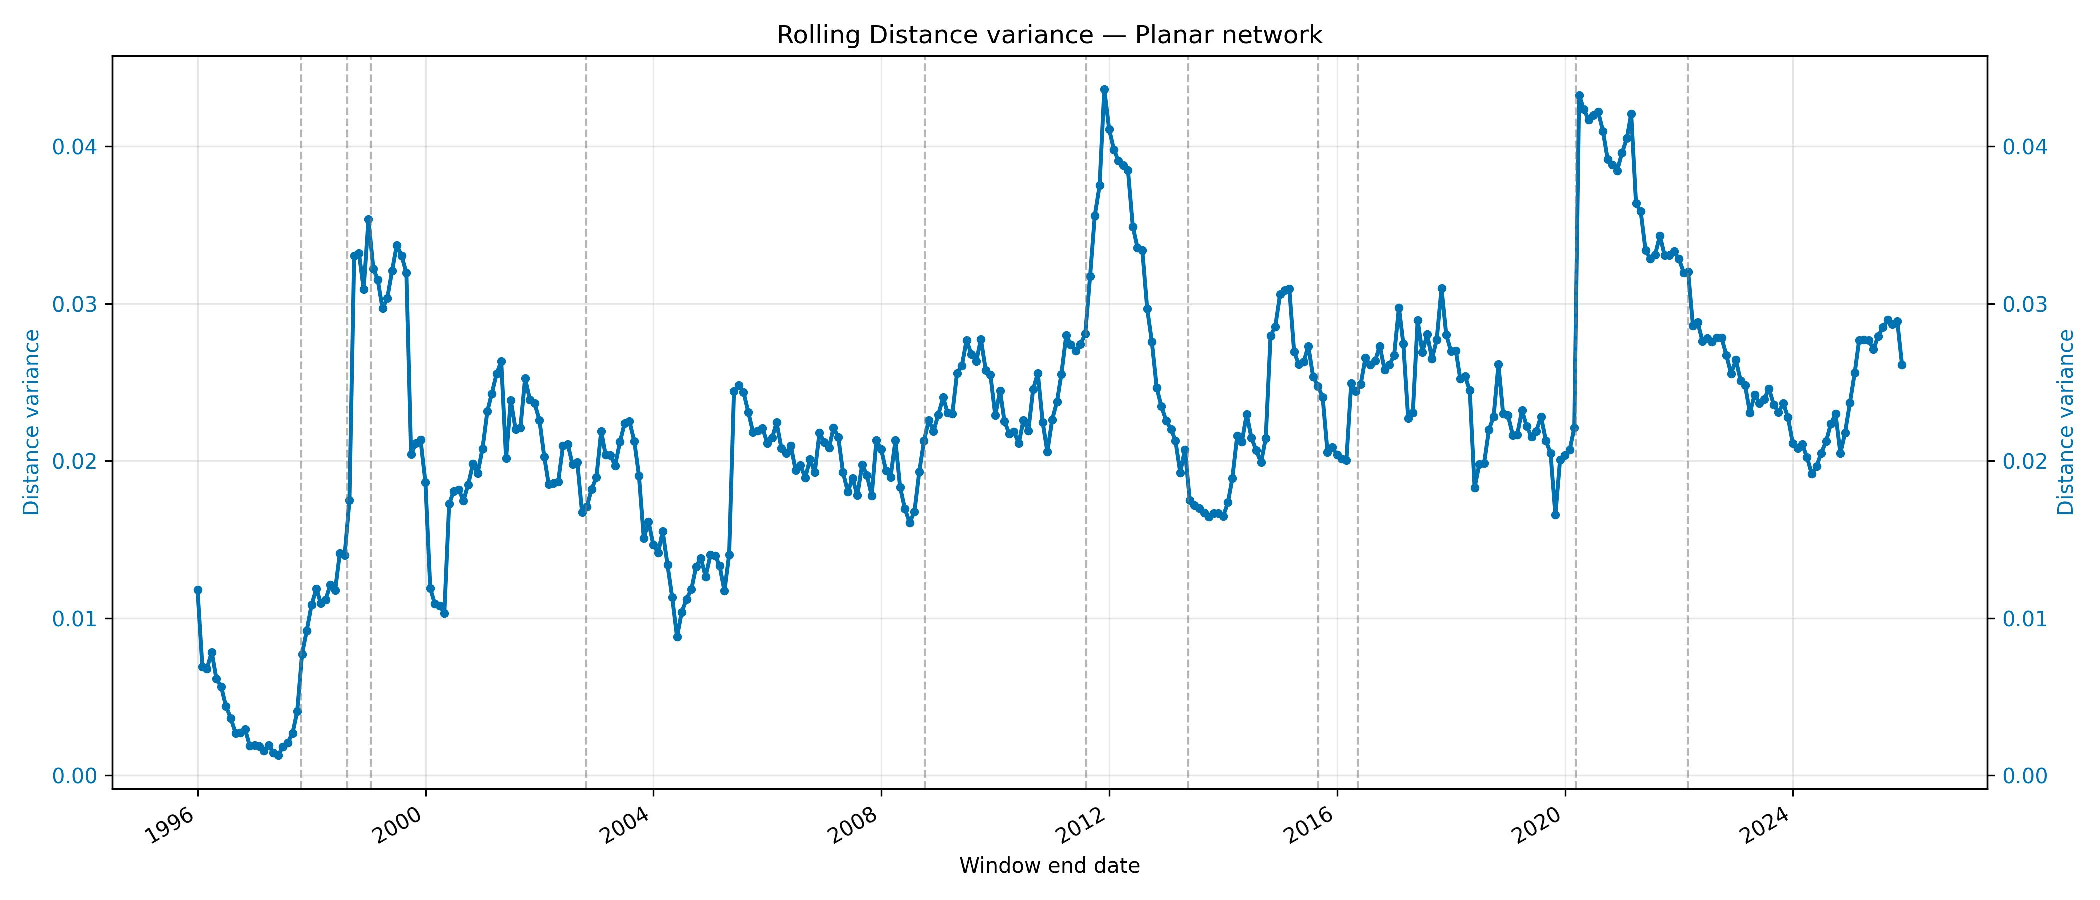
\includegraphics[width=\linewidth,keepaspectratio]{figures/networks/Planar_dist_var_evolucao.pdf}
    \caption{Distance variance.}
    \label{fig:planar-dist-var}
\end{subfigure}
\caption{Mean and variance of PMFG edge distances across the 360 rolling windows. These raw quantities provide geometric context for compression and dispersion changes.}
\label{fig:planar-dist-moments-a}
\end{center}

The first pair of distance panels separates the location and spread of PMFG edge distances. The mean captures compression of the retained geometry, while the variance records whether that compression is accompanied by redistribution across edges. These are raw context measures and are interpreted with, not instead of, the size-conditioned results.

\begin{center}
\captionsetup{type=figure}
\centering
\begin{subfigure}{0.99\linewidth}
    \centering
    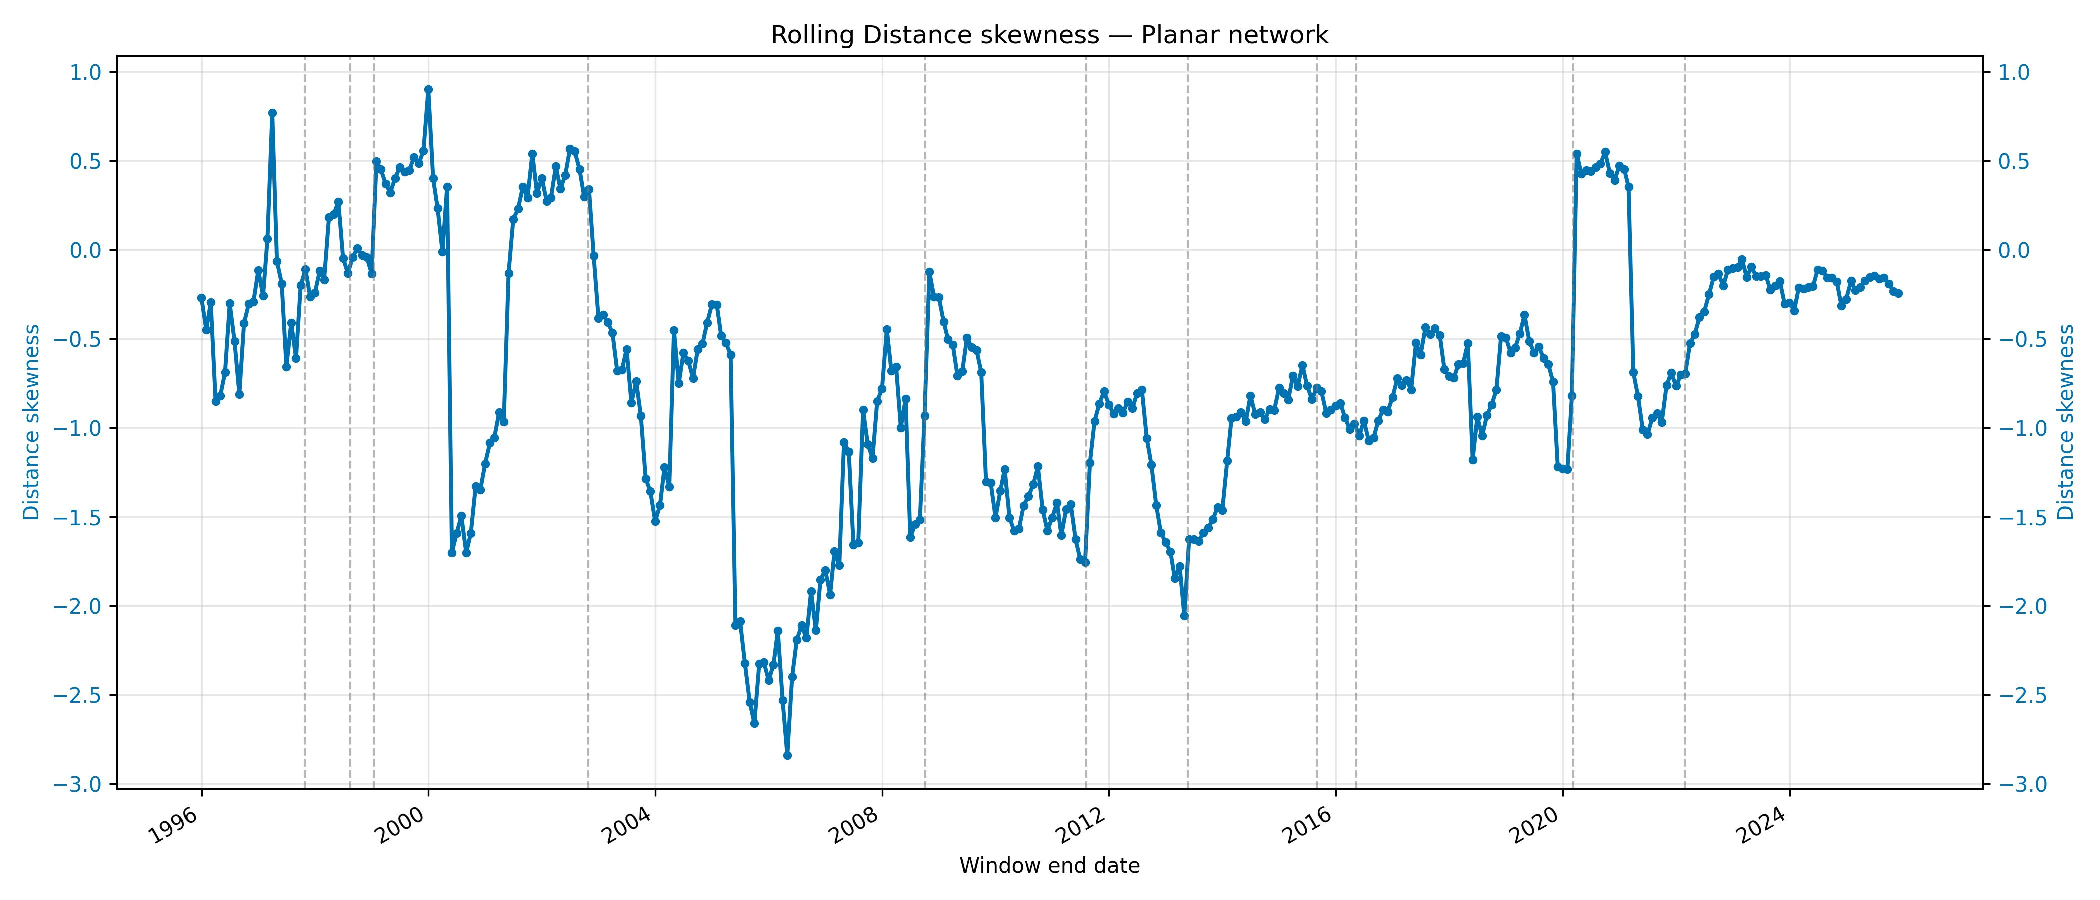
\includegraphics[width=\linewidth]{figures/networks/Planar_dist_skew_evolucao.pdf}
    \caption{Distance skewness.}
    \label{fig:planar-dist-skew}
\end{subfigure}

\begin{subfigure}{0.99\linewidth}
    \centering
    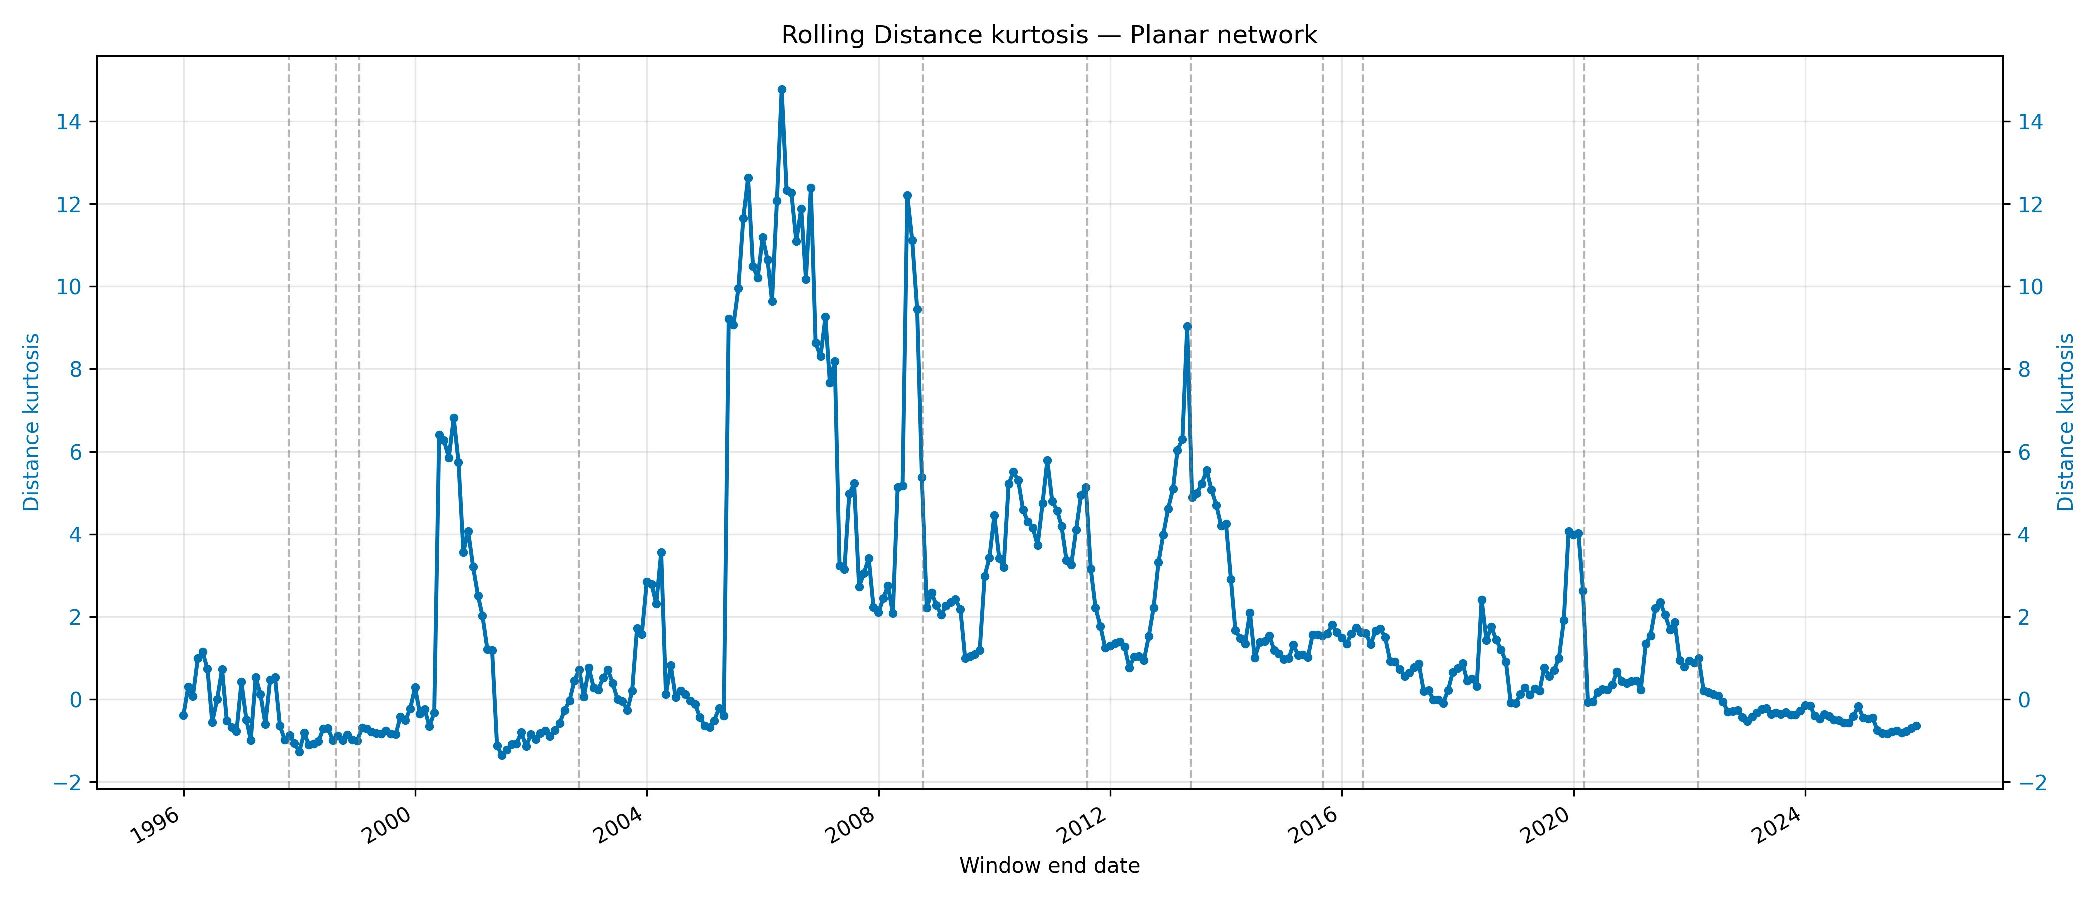
\includegraphics[width=\linewidth]{figures/networks/Planar_dist_kurt_evolucao.pdf}
    \caption{Distance kurtosis.}
    \label{fig:planar-dist-kurt}
\end{subfigure}
\caption{Skewness and kurtosis of PMFG edge distances across the 360 rolling windows. These raw distributional moments characterize reorganization beyond changes in the mean and variance and are interpreted alongside the size-conditioned topology comparisons.}
\label{fig:planar-dist-moments-b}
\end{center}

The skewness and kurtosis panels add asymmetry and tail concentration to the distance description. Their event-level signs are not forced to agree with the mean or variance, which is why the manuscript reports the full four-moment family rather than reducing the topology to a single distance index.

Representative planar snapshots in Figure~\ref{fig:planar-snapshots} make the same point visually: the first and last windows show that the market does not merely gain or lose edges; it reorganizes its geometry.

\begin{sidewaysfigure}[p]
\centering
\begin{subfigure}{0.49\textheight}
    \centering
    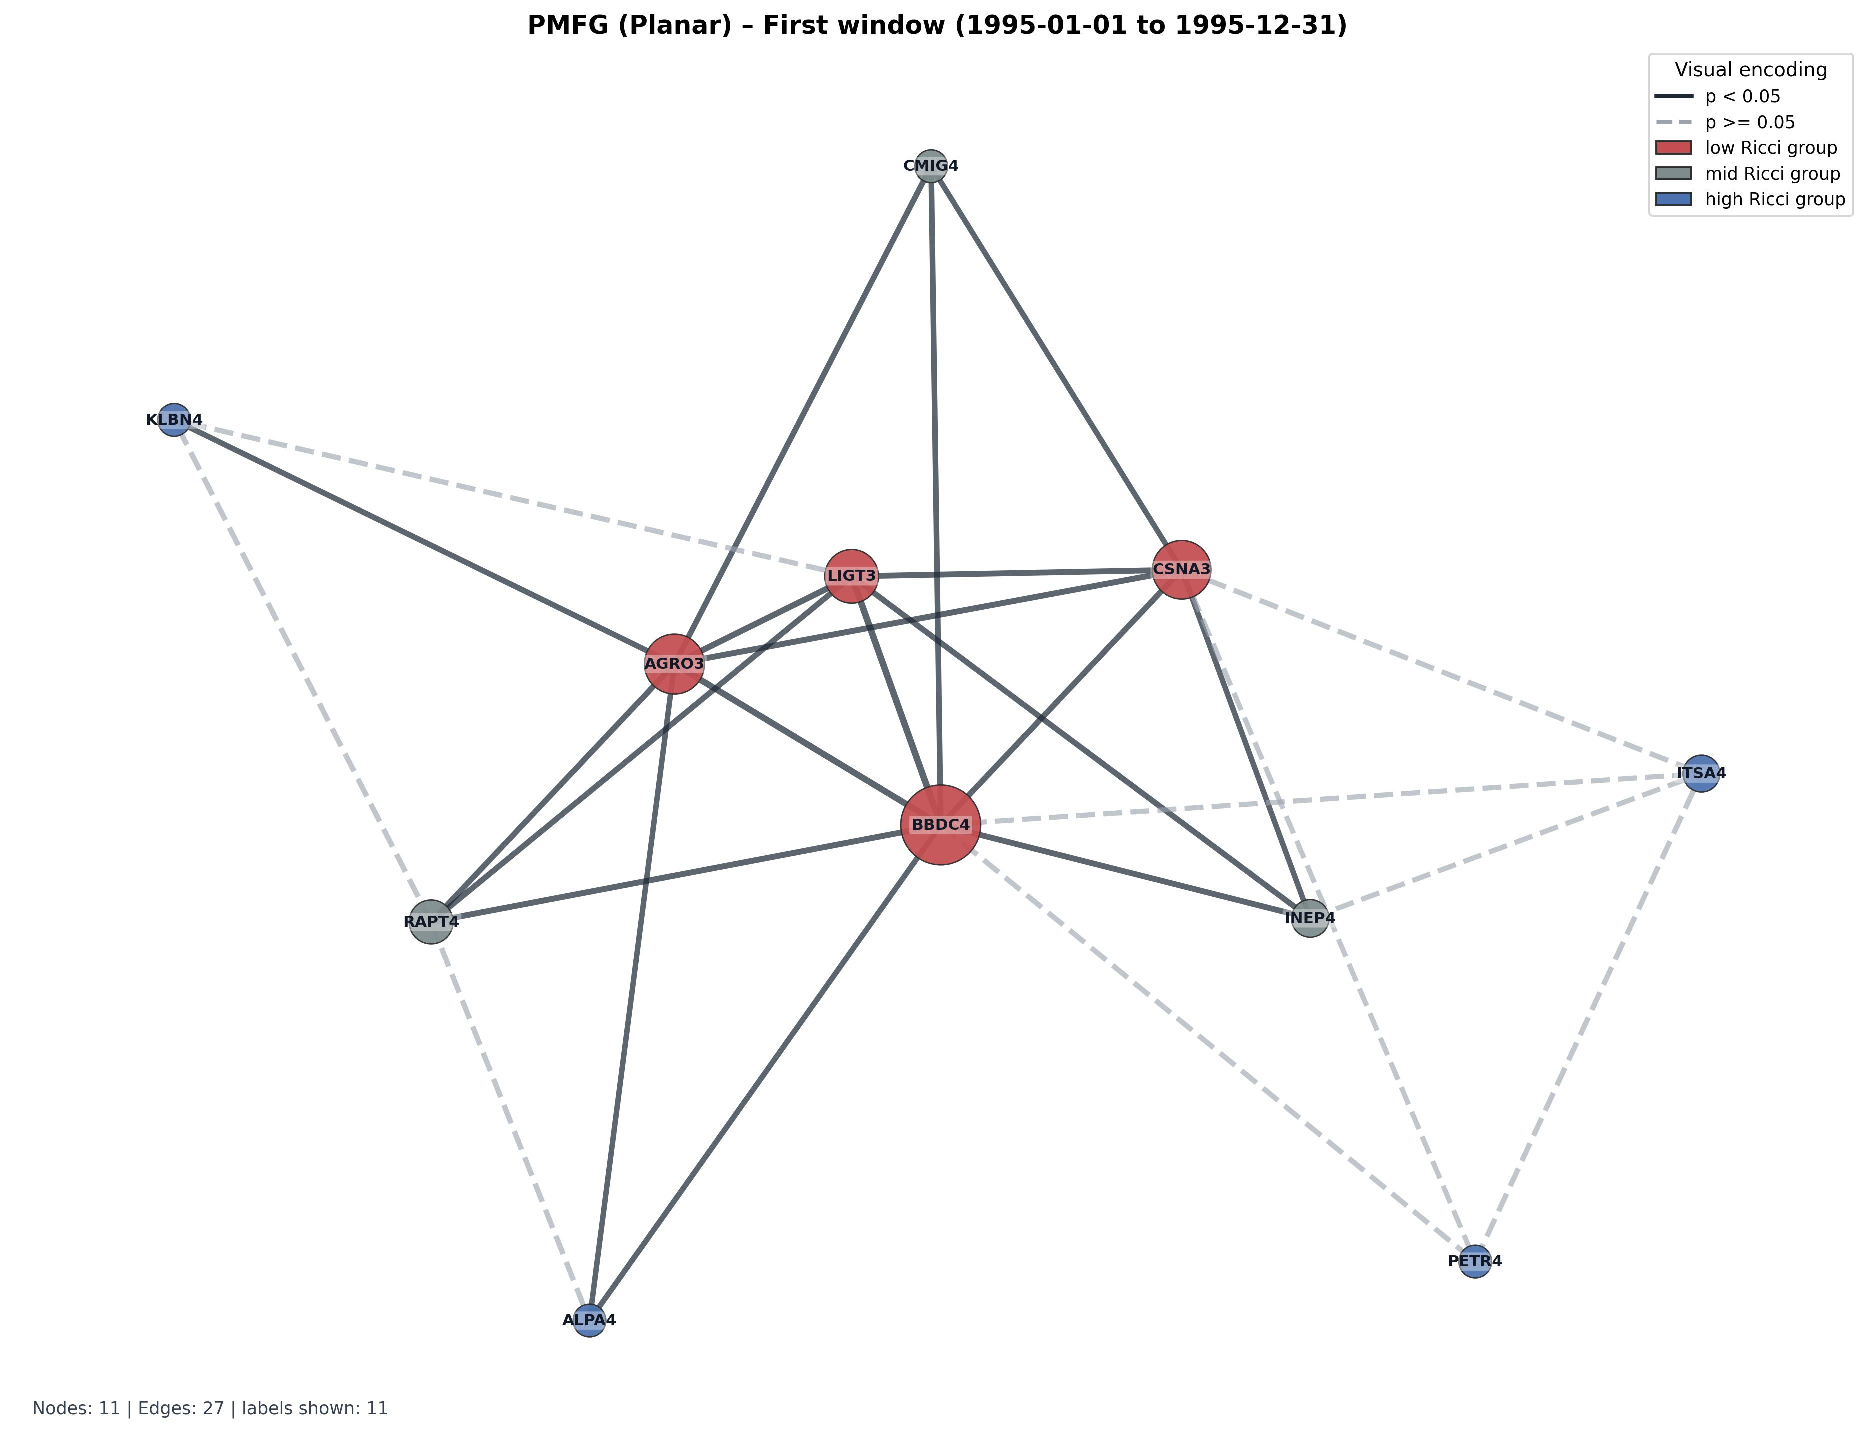
\includegraphics[width=\linewidth,trim=35 35 35 35,clip,keepaspectratio]{figures/networks/planar_pval_primeira_janela.pdf}
    \caption{Planar network, first window.}
\end{subfigure}\hfill%
\begin{subfigure}{0.49\textheight}
    \centering
    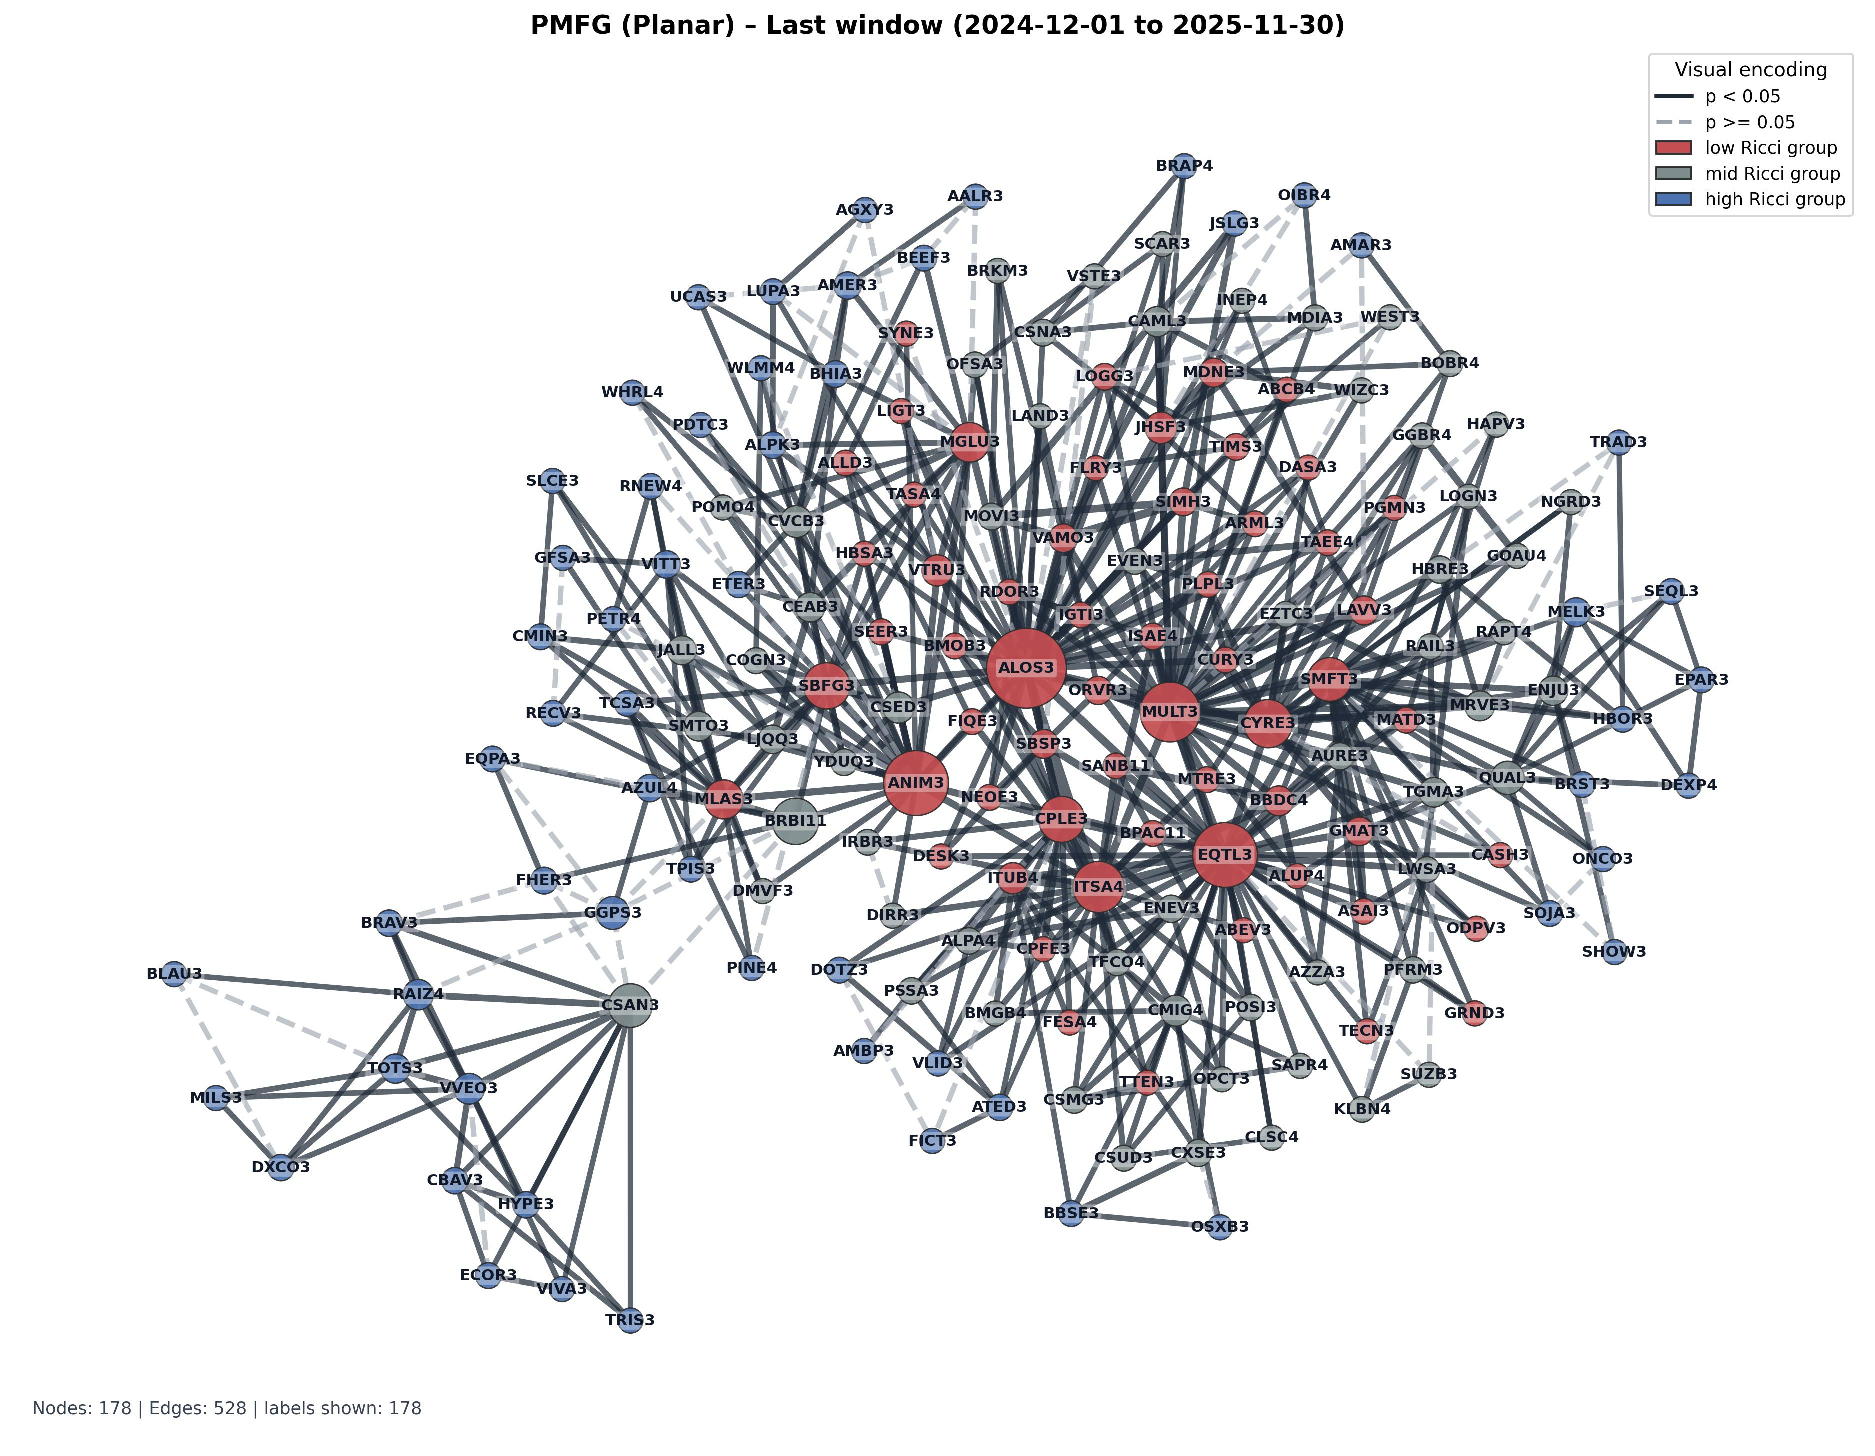
\includegraphics[width=\linewidth,trim=35 35 35 35,clip,keepaspectratio]{figures/networks/planar_pval_ultima_janela.pdf}
    \caption{Planar network, last window.}
\end{subfigure}
\caption{Representative planar financial networks (PMFG extracted from the full distance matrix, without p-value pre-filtering). Node size is proportional to betweenness centrality; node colour identifies the PMFG community. Solid edges indicate statistically significant pairs ($p < 0.05$); dashed edges indicate topologically retained but weaker pairs ($p \geq 0.05$). The comparison between the first and last windows illustrates how planar topology evolves with the growing and maturing B3 universe.}
\label{fig:planar-snapshots}
\end{sidewaysfigure}

The two snapshots give an interpretable visual endpoint to the rolling planar diagnostics. They show that changes in the B3 universe involve both the retained edge geometry and the arrangement of communities. Because they compare only two windows, they are illustrative and must be read alongside the 360-window trajectories and the phase tables.

\subsection{Phase Configurations Across Four Configured Events}
\label{subsec:phase-configurations}

The primary comparison uses four pre-specified daily IBOVESPA $-3\sigma$ shock triggers as externally dated anchors: 27 October 1997 (Asian crisis), 27 August 1998 (Russian default/LTCM), 29 September 2008 (Global Financial Crisis), and 9 March 2020 (COVID-19). Thus, the shock months are October 1997, August 1998, September 2008, and March 2020, respectively. These dates are trigger anchors for the rolling-window comparison; they are not asserted to be the largest one-day losses within separately delimited crisis episodes. For each anchor, a tranquil reference formed by all rolling windows outside its local pre-event, event-containing, and post-event phases is reported alongside six local pre-event windows, 12 event-containing windows, and six post-event windows. Distance moments and PMFG modularity are raw descriptive context; Ward-group and PMFG-community quantities and centralities are interpreted as size-conditioned residuals; KS and Marchenko--Pastur diagnostics characterize the correlation-matrix layer. Mean PMFG degree is excluded from substantive comparisons because maximal planarity fixes it at $6-12/N_t$.

The phase assignment is based on the dated 12-month rolling samples, not on an inferred crisis onset. A pre-event sample must end strictly before its shock day; the six pre-event samples end in April--September 1997, February--July 1998, March--August 2008, and September 2019--February 2020 for the four anchors, respectively. Hence, the latest pre-event sample ends in the calendar month immediately preceding the shock month and contains no return observed on or after the shock date. An event-containing sample has $\mathrm{Window\_Start}\leq\mathrm{shock\ date}\leq\mathrm{Window\_End}$; the 12 such overlapping samples therefore contain the shock observation but also preceding observations. Post-event samples begin strictly after the shock day, beginning in November 1997, September 1998, October 2008, and April 2020, respectively. This construction makes the local contrasts chronological, while the one-year rolling span requires them to remain descriptive rather than instantaneous effects.

Figure~\ref{fig:four-state-crisis-infographic} translates the phase protocol into four operational states for each configured event. The observed shock date marks the rupture between the pre-event and crisis states; it is not itself a state or an estimated irreversible threshold. The phase profiles display observed means across tranquil, pre-event, event-containing, and post-event states for complementary diagnostics, retaining heterogeneous metric responses rather than imposing a common sequence.

\begin{sidewaysfigure}[p]
\centering
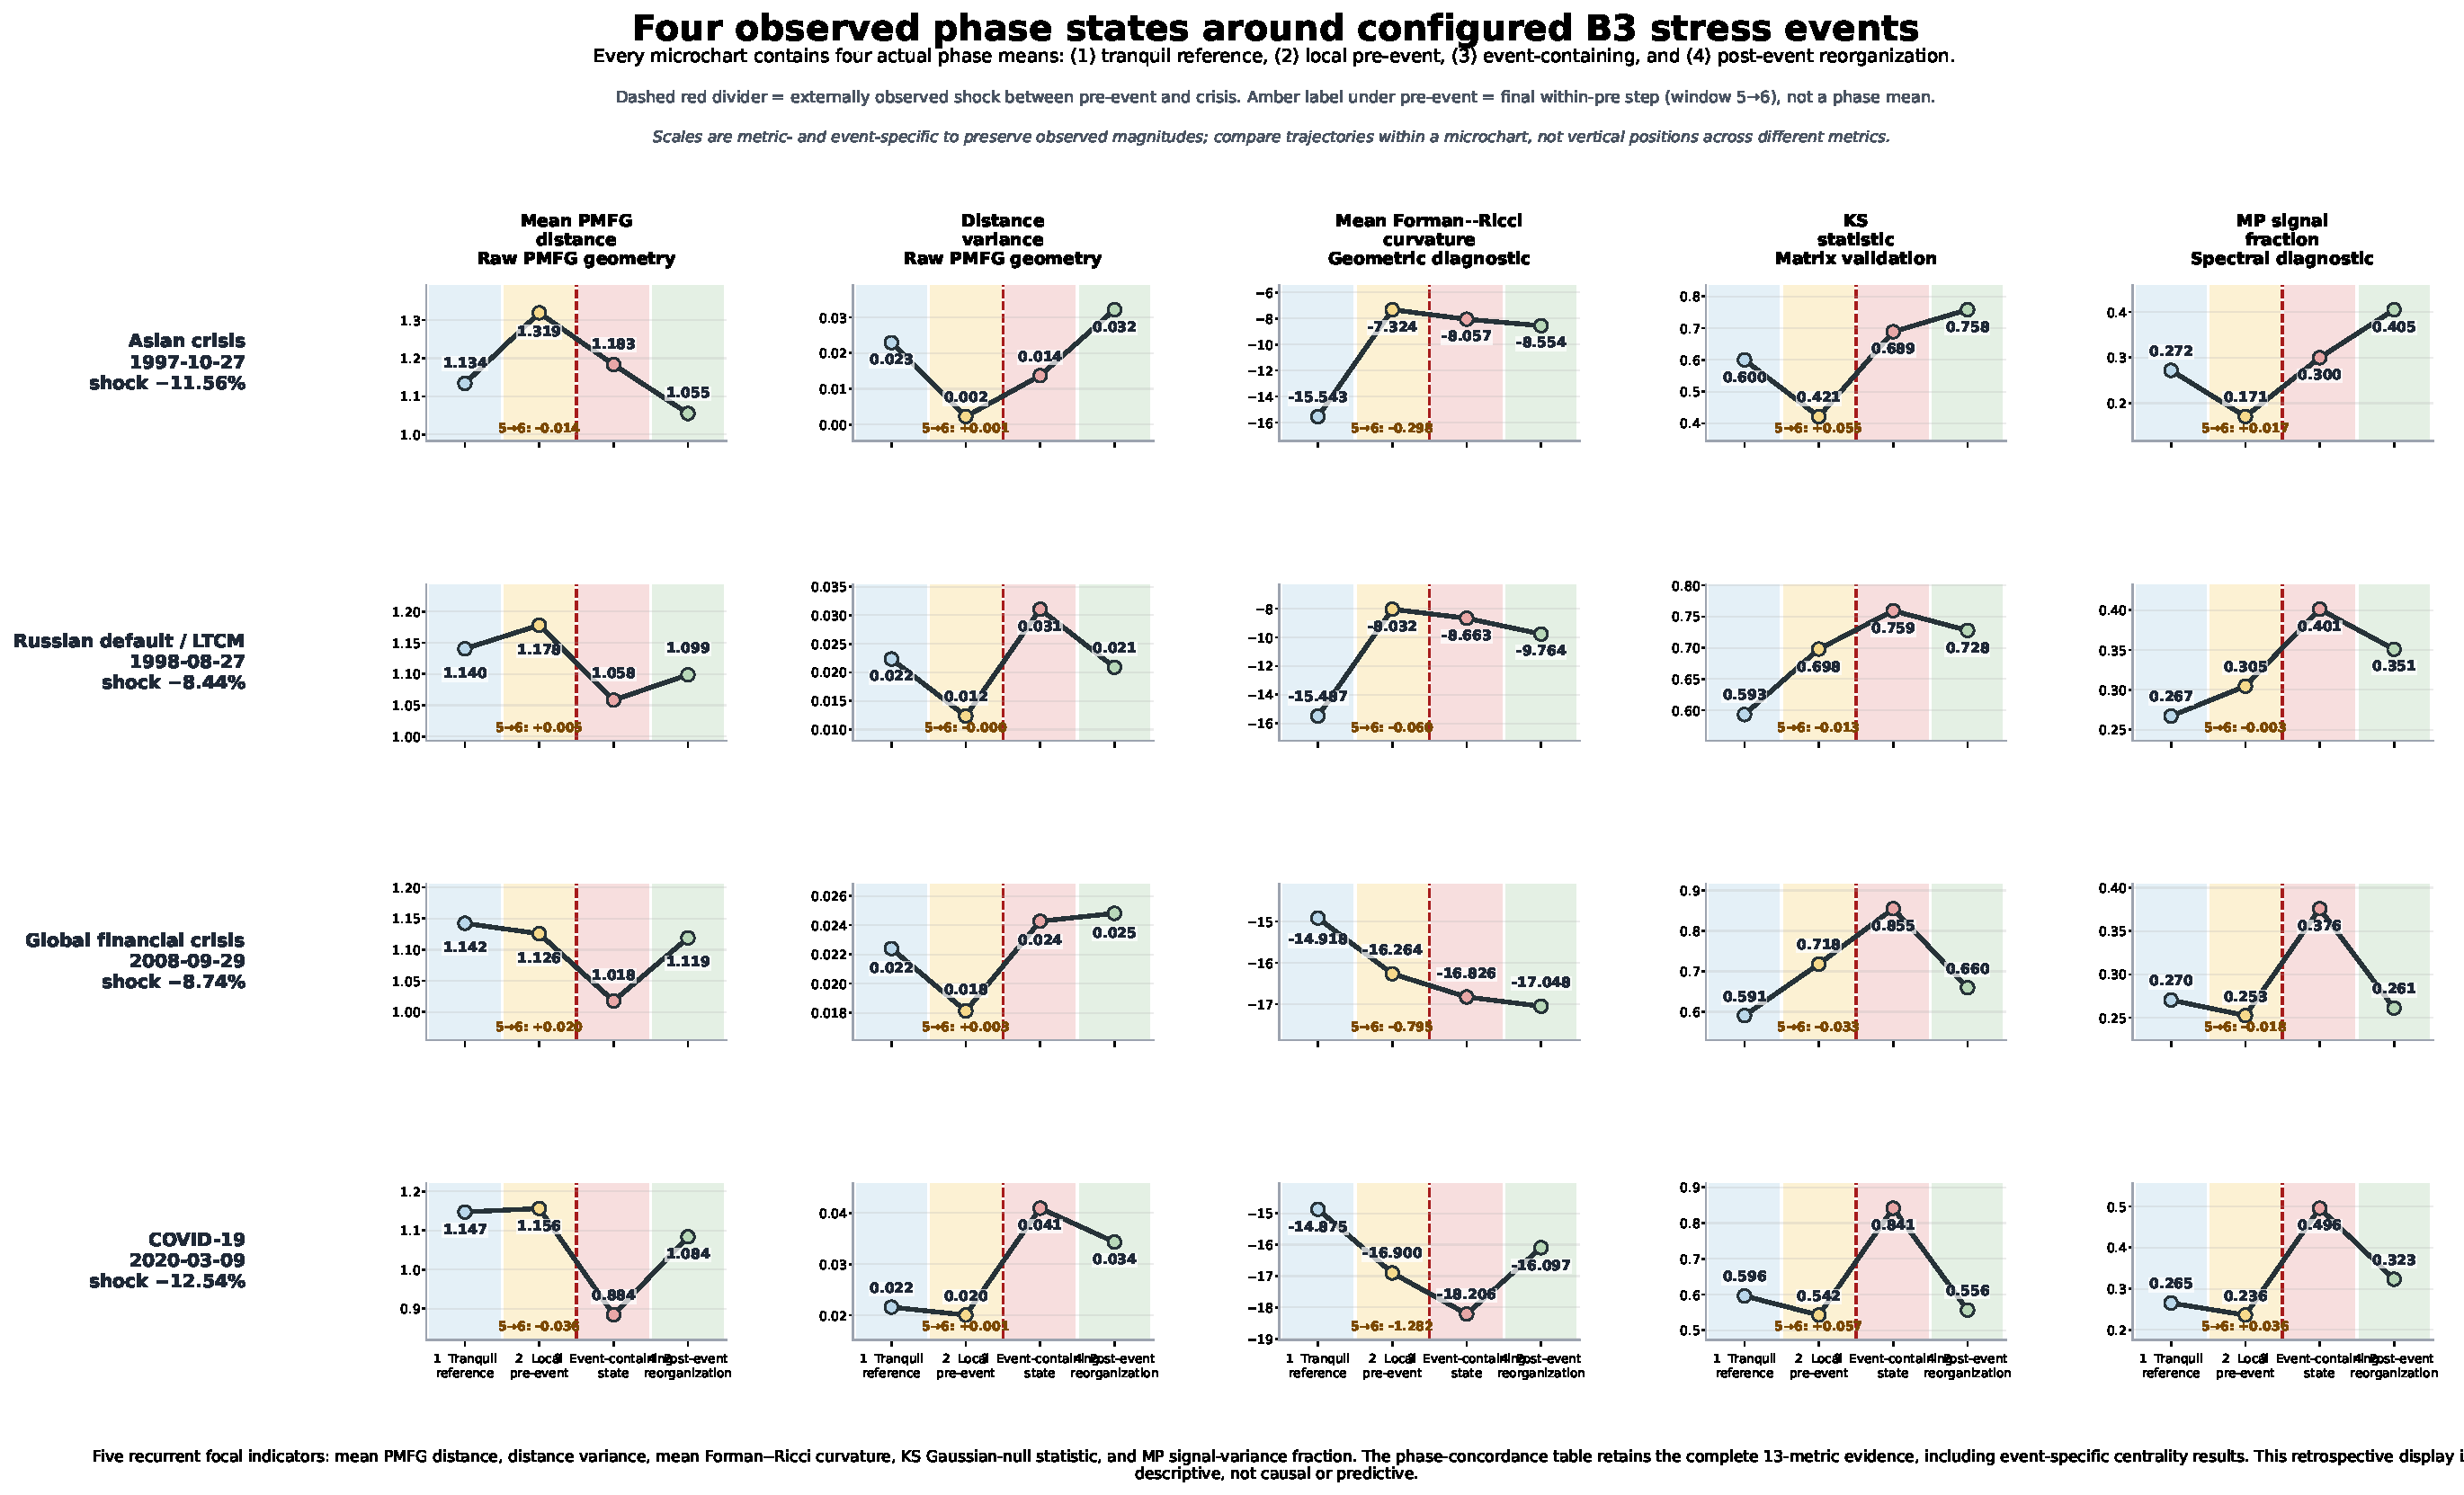
\includegraphics[width=\textheight,height=\textwidth,keepaspectratio]{figures/infographics/four_state_crisis_infographic.pdf}
\caption{Observed four-state phase profiles around the four configured B3 stress events. Each microchart plots the pipeline means for tranquil, local pre-event, event-containing, and post-event states for five focal diagnostics: mean PMFG distance, distance variance, mean Forman--Ricci curvature, KS Gaussian-null displacement, and MP signal-variance fraction. The additional Ricci column provides a geometric diagnostic alongside the distance, matrix, and spectral measures; it is interpreted descriptively rather than as a universal curvature-based crisis marker. The dashed divider locates the externally observed shock trigger between local pre-event and event-containing states; where shown, the amber label reports the defined fifth-to-sixth within-pre-window difference rather than a phase mean. Scales are metric- and event-specific, so each profile supports within-metric comparison across the four states. Table~\ref{tab:phase-concordance-core} retains the complete 13-metric four-crash core-panel evidence, including event-specific centrality results. This retrospective display is descriptive, not causal or predictive.}
\label{fig:four-state-crisis-infographic}
\end{sidewaysfigure}

Table~\ref{tab:phase-transitions} provides the compact transition summary for the four configured core events, the additional 1999 $-3\sigma$ trigger, and the full eleven-anchor sensitivity calendar. It is read together with the event-level phase profiles above: the table summarizes directional recurrence, whereas the profiles retain event-specific magnitudes and heterogeneity.

\begin{table}[width=\textwidth,pos=h]
\centering
\caption{Descriptive phase-transition states across the four configured events and the sensitivity calendar. The tranquil reference contains all rolling windows outside the local pre-event, event-containing, and post-event phases. For each daily shock anchor, the six pre-event 12-month samples end strictly before the shock day; the 12 event-containing samples span the shock day; and the six post-event samples begin strictly after it. Counts for the 11-anchor row combine five actual $-3\sigma$ triggers and six fallback proxies, and hence remain a sensitivity result. Arrows express observed phase contrasts, not temporal causality or predictive performance.}
\label{tab:phase-transitions}
\scriptsize
\setlength{\tabcolsep}{4pt}
\renewcommand{\arraystretch}{1.12}
\begin{tabular*}{\tblwidth}{@{}p{0.16\textwidth}p{0.25\textwidth}p{0.25\textwidth}p{0.25\textwidth}@{}}
\toprule
Transition & Four configured events & Five actual $-3\sigma$ triggers & Eleven-anchor sensitivity calendar \\
\midrule
Tranquil $\rightarrow$ pre & No common pre-state is evaluated as a transition signature. & No predictive interpretation. & Ward residual is lower in pre in $10/11$; KS and both MP fractions are lower in only $7/11$, while distance mean and betweenness are split. \\
Pre $\rightarrow$ during & Distance mean $\downarrow$ and distance variance, skewness, KS, MP signal, and market mode $\uparrow$ in $4/4$. & The same six contrasts occur in $5/5$. & Distance mean $\downarrow$ in $9/11$; variance $\uparrow$ in $8/11$; skewness $\uparrow$ in $9/11$; KS $\uparrow$ in $10/11$; MP signal $\uparrow$ in $8/11$; market mode $\uparrow$ in $9/11$. \\
During $\rightarrow$ post & Relative to pre, lower distance mean and higher variance and MP signal persist in $4/4$; other families are event-specific. & Relative to pre, distance mean remains lower in $4/5$ and variance and MP signal higher in $4/5$. & Relative to pre, distance mean remains lower in $8/11$, KS and MP signal higher in $8/11$, and skewness higher in $7/11$; variance and market mode are heterogeneous. \\
\bottomrule
\end{tabular*}
\end{table}


The infographic is the visual reference for the phase vocabulary used in the tables. It separates the tranquil benchmark from the three local states and makes explicit that the event-containing state consists of overlapping rolling windows. The figure therefore clarifies the timing convention without implying that the shock date is an estimated threshold or that the post-event state is a recovery state.

Table~\ref{tab:phase-concordance-core} summarizes the two local-pre-referenced contrasts (event-containing minus pre-event and post-event minus pre-event) derived from the four-state protocol; it does not replace the tranquil and pre-event phase means displayed in Figure~\ref{fig:four-state-crisis-infographic}. The 11-anchor sensitivity analysis is presented through Figures~\ref{fig:proxy-11-non-ricci}--\ref{fig:proxy-11-pre-trajectories}, with its tables and interpretation integrated into the Results section. Within the four configured core events, mean PMFG distance falls and distance variance, KS displacement, MP signal fraction, and market-mode fraction rise in all four event-containing versus pre-event comparisons; the additional 1999 trigger is retained as a sensitivity anchor, and the six fallback proxies are more heterogeneous (Table~\ref{tab:phase-concordance} and Figures~\ref{fig:proxy-11-non-ricci}--\ref{fig:proxy-11-ricci}).

\begin{sidewaysfigure}[p]
\captionsetup{type=figure}
\centering
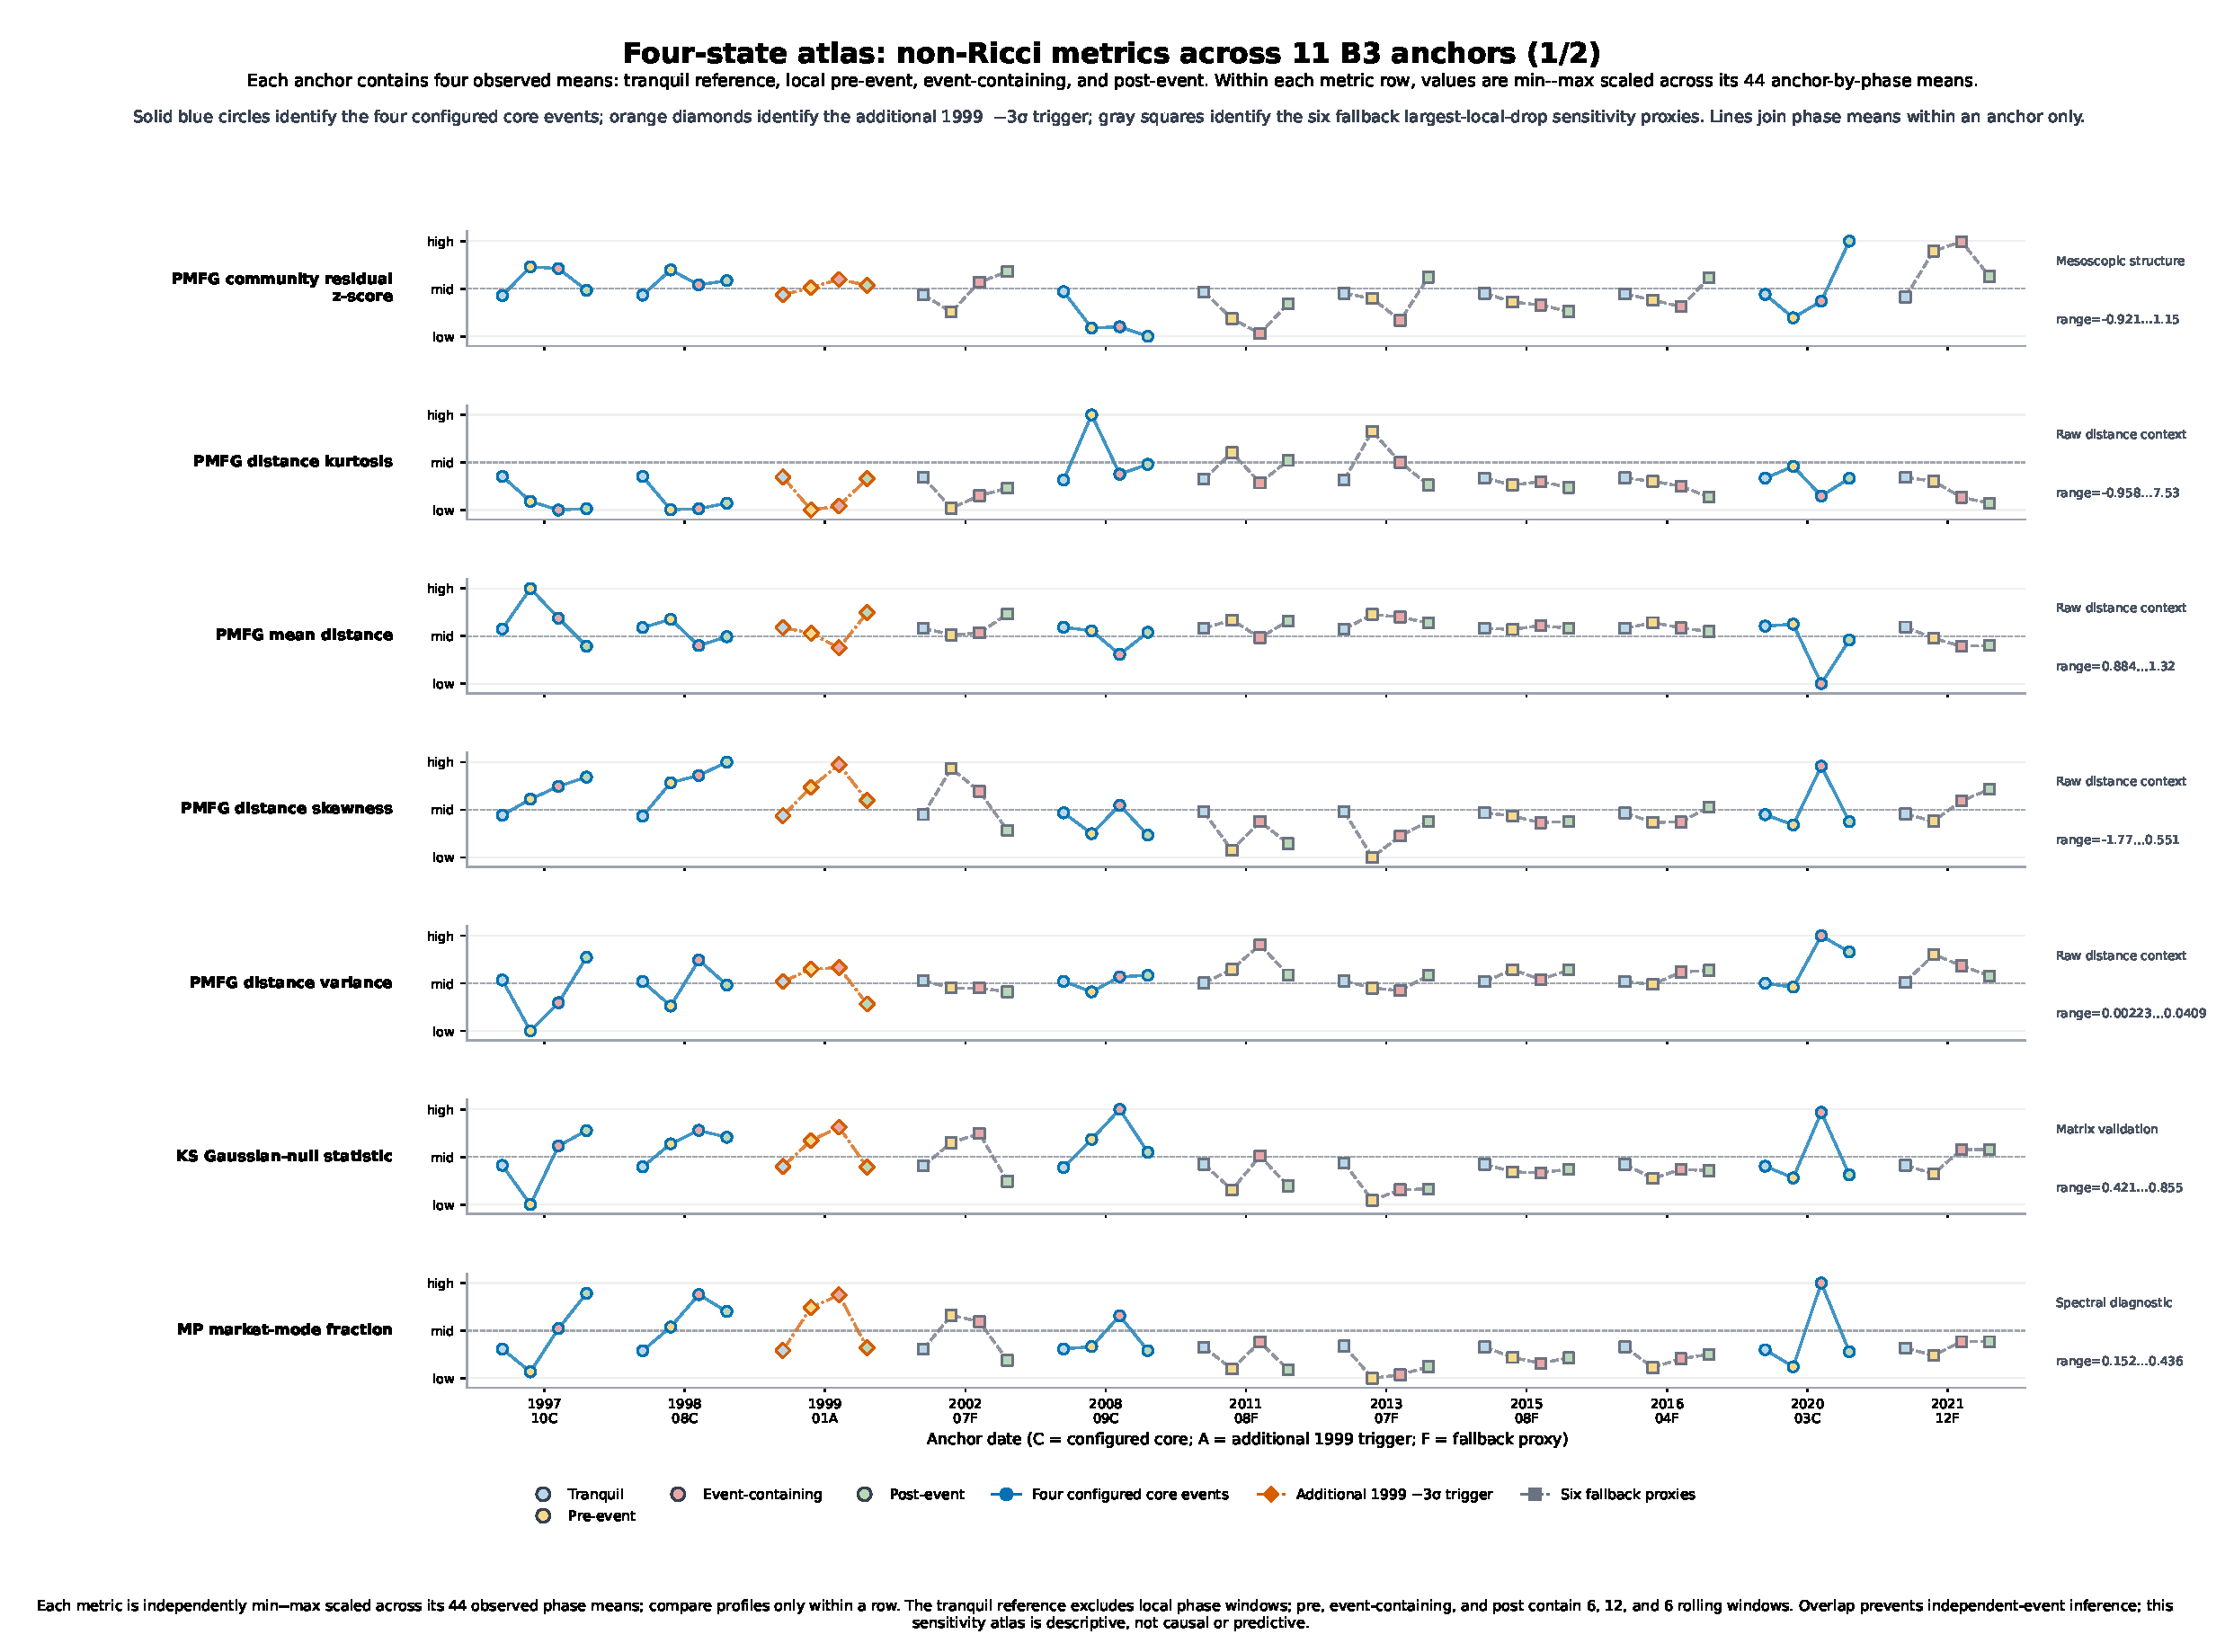
\includegraphics[width=0.90\textheight,height=0.86\textwidth,keepaspectratio]{figures/validation/proxy_11_non_ricci_metric_contrasts_part1.pdf}
\caption{Four-state sensitivity atlas of the first seven non-curvature metrics across 11 B3 anchors. Solid blue circles mark the four configured core events, orange diamonds mark the additional 1999 $-3\sigma$ trigger, and grey squares mark the six fallback proxies; line style and marker shape repeat the distinction without relying on colour alone.}
\label{fig:proxy-11-non-ricci}
\end{sidewaysfigure}

\begin{sidewaysfigure}[p]
\ContinuedFloat
\centering
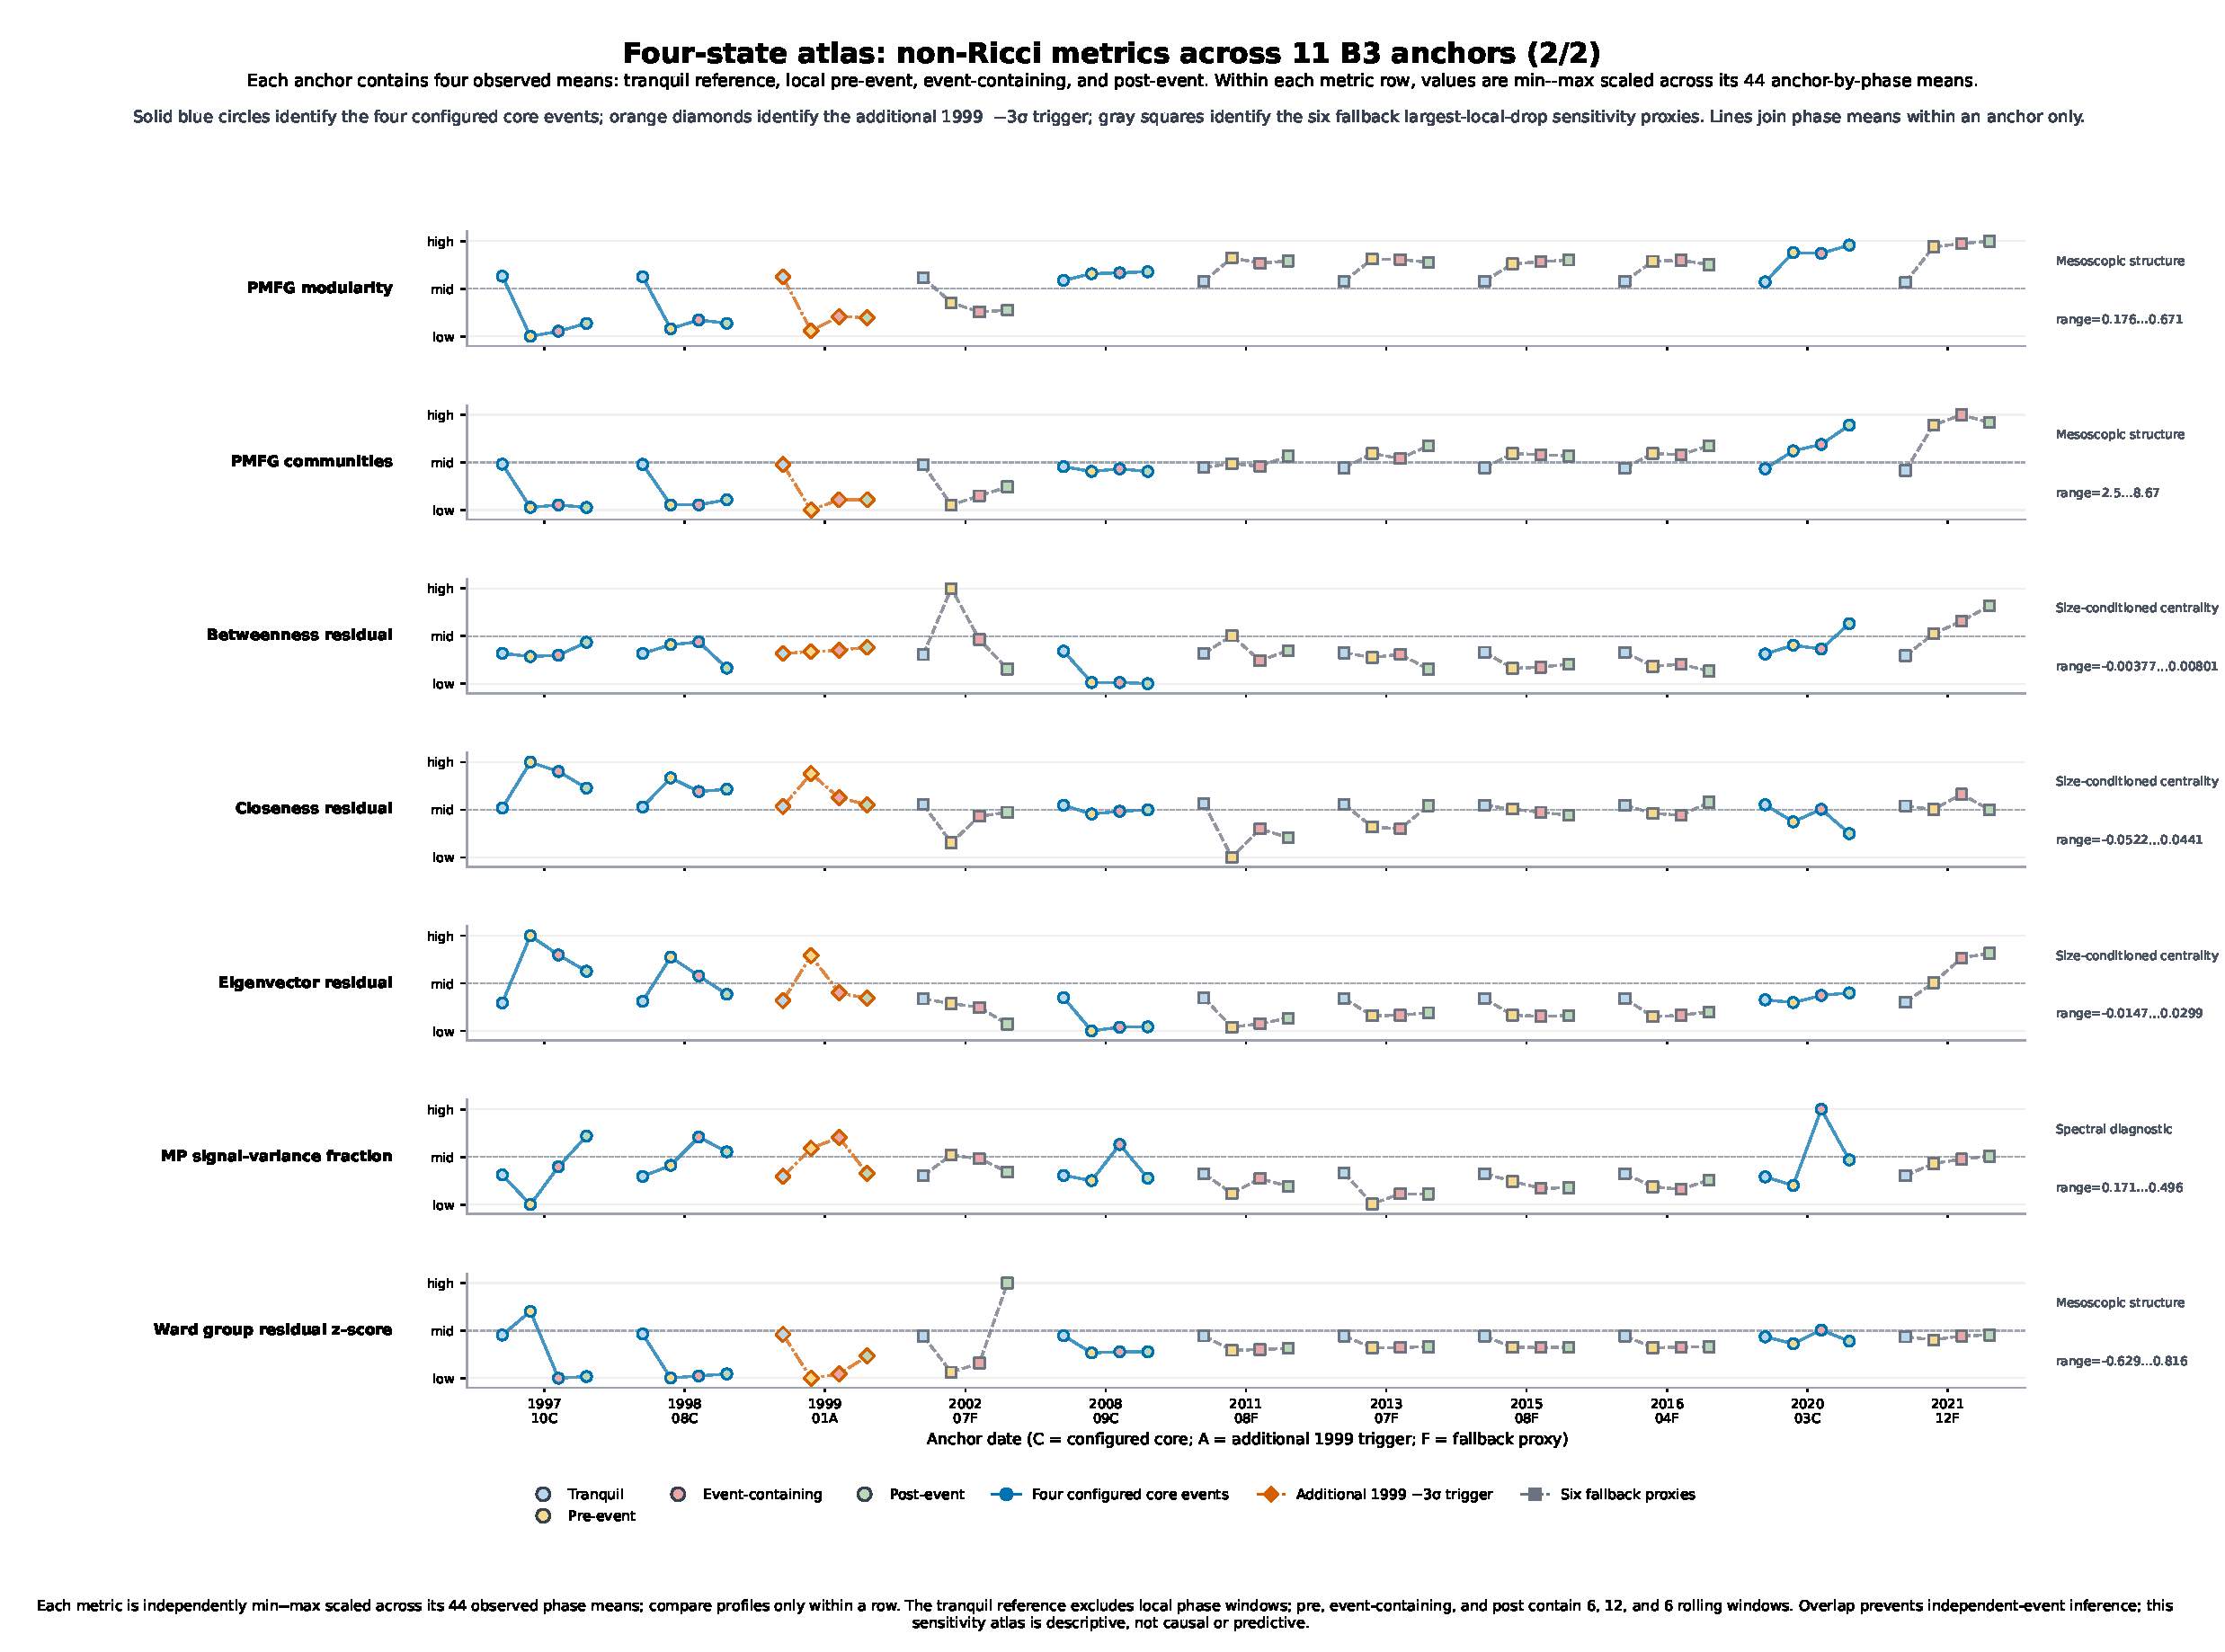
\includegraphics[width=0.90\textheight,height=0.86\textwidth,keepaspectratio]{figures/validation/proxy_11_non_ricci_metric_contrasts_part2.pdf}
\caption[]{Four-state sensitivity atlas (continued): remaining seven non-curvature metrics.}
\end{sidewaysfigure}

\begin{sidewaysfigure}[p]
\captionsetup{type=figure}
\centering
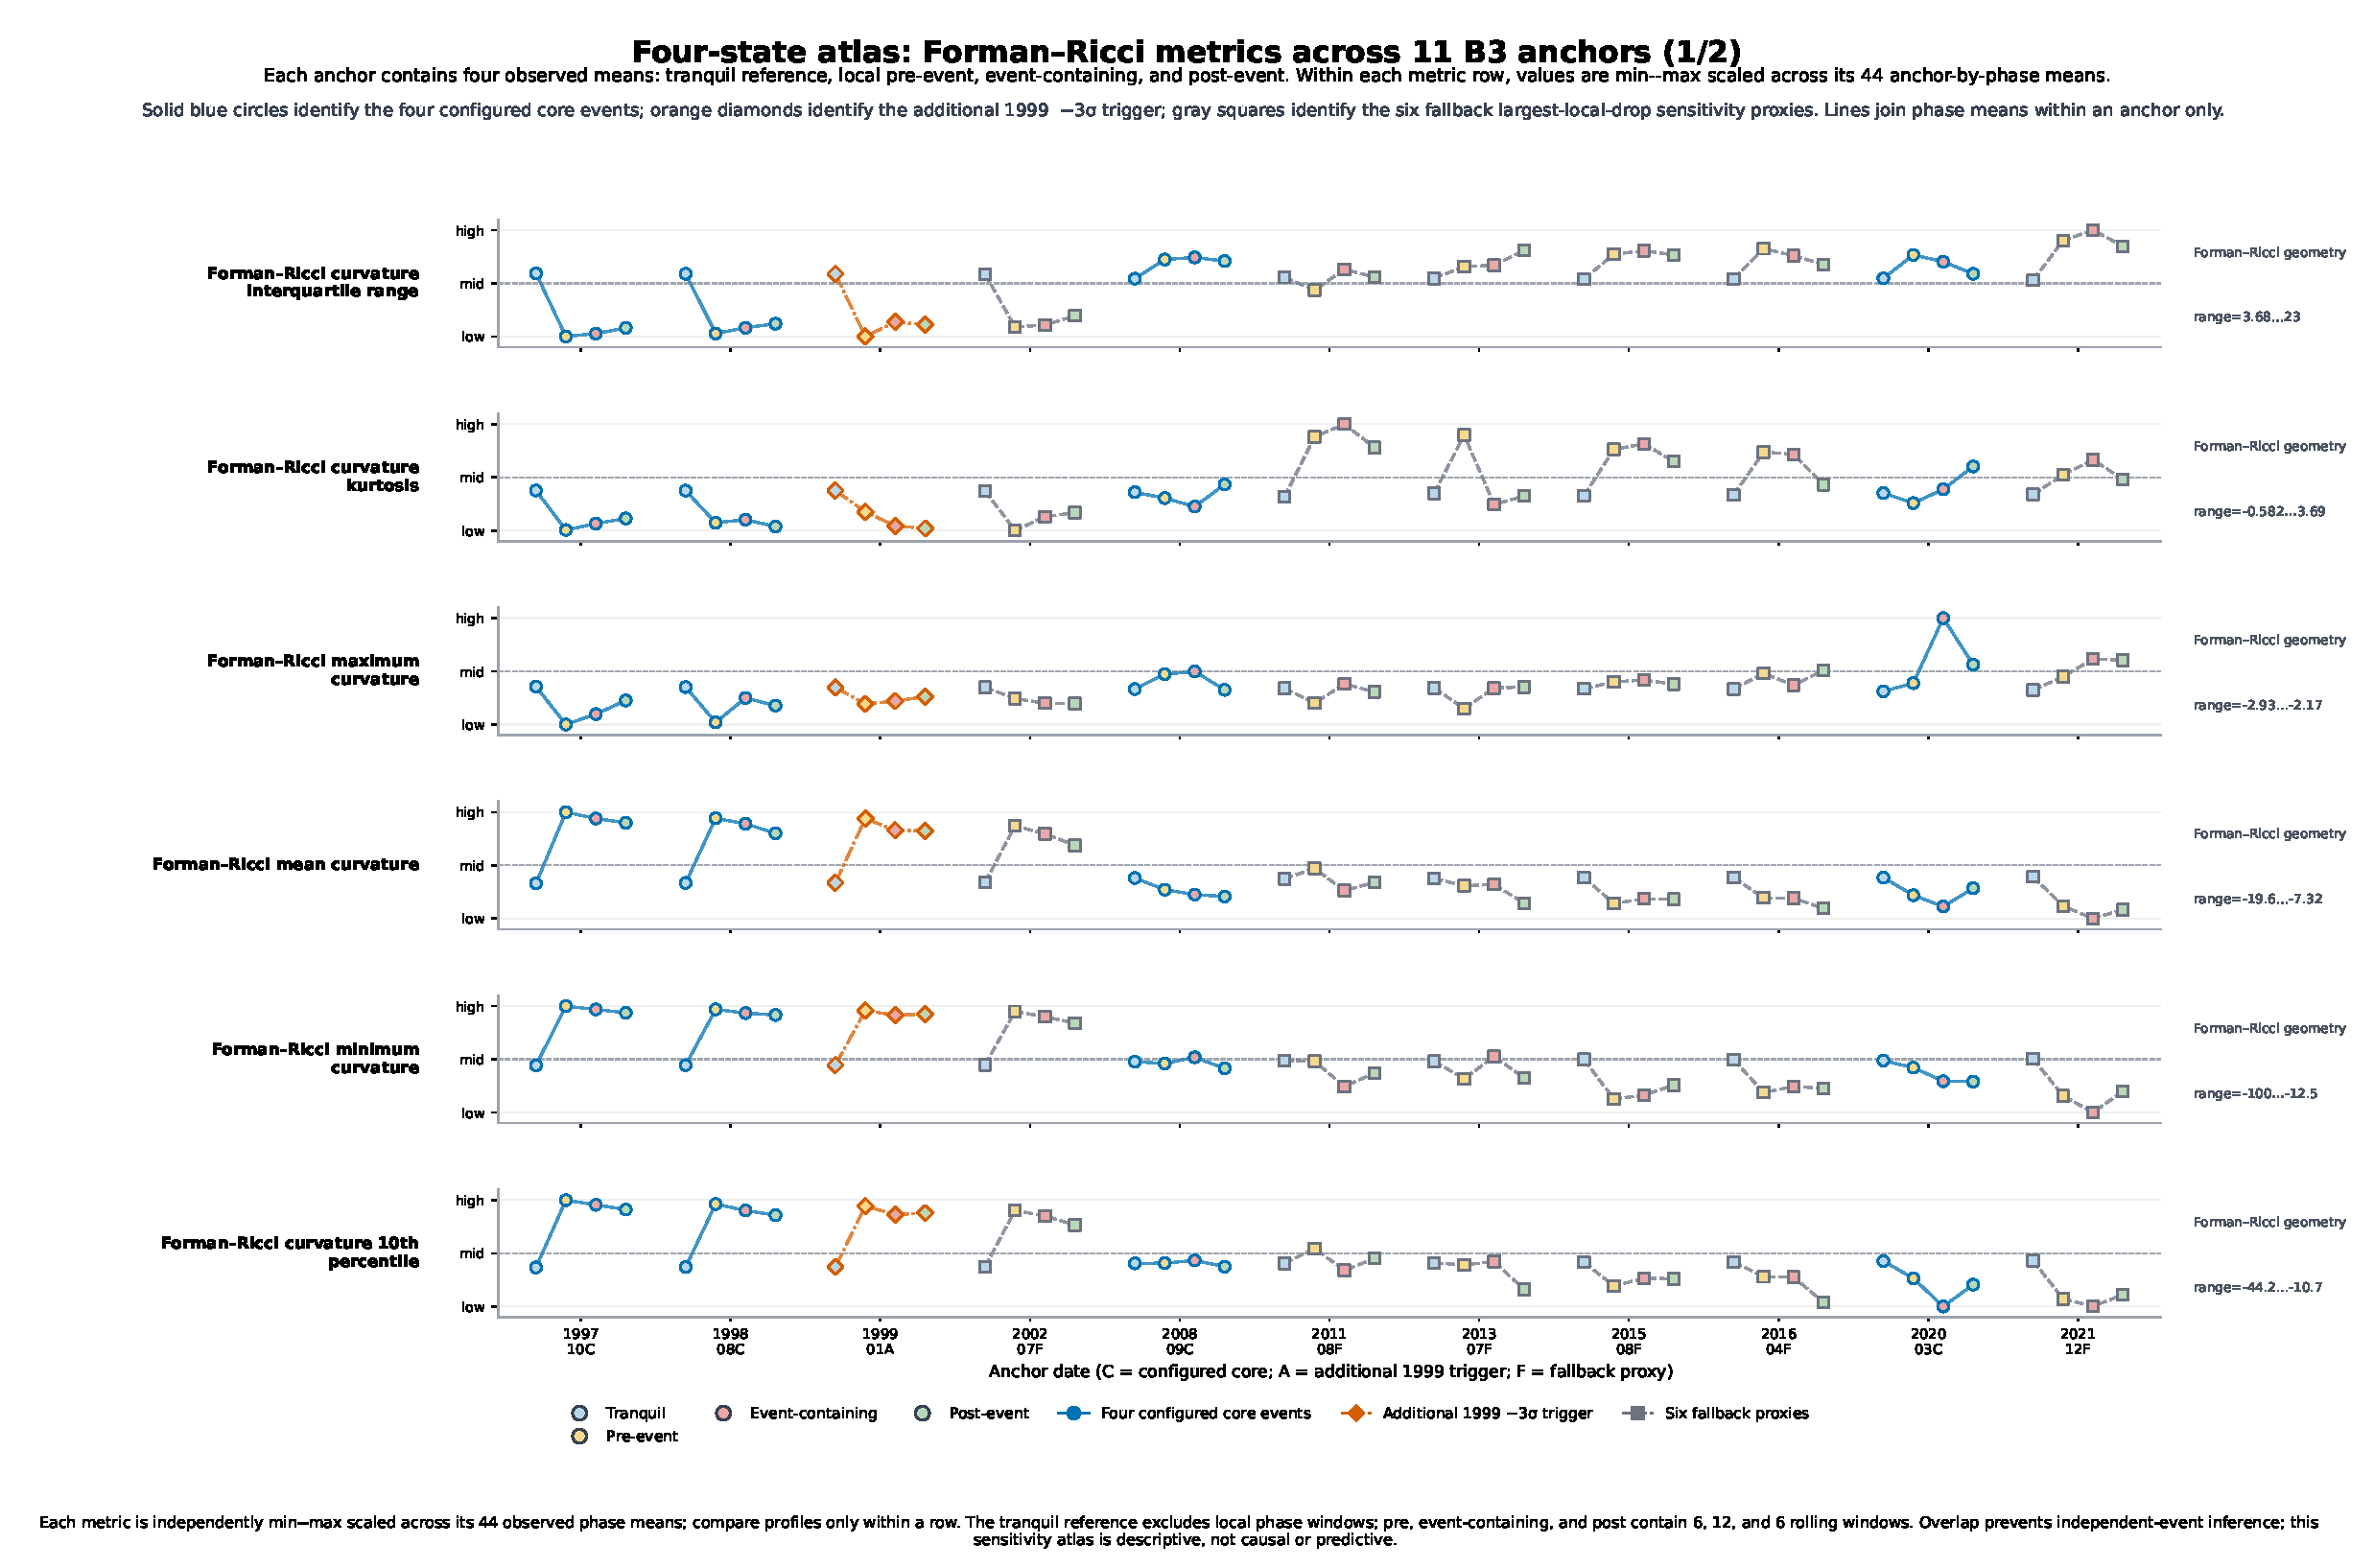
\includegraphics[width=0.90\textheight,height=0.86\textwidth,keepaspectratio]{figures/validation/proxy_11_ricci_metric_contrasts_part1.pdf}
\caption{Four-state sensitivity atlas of the first six Forman--Ricci metrics across 11 B3 anchors. Solid blue circles mark the four configured core events, orange diamonds mark the additional 1999 $-3\sigma$ trigger, and grey squares mark the six fallback proxies; line style and marker shape repeat the distinction without relying on colour alone.}
\label{fig:proxy-11-ricci}
\end{sidewaysfigure}

\begin{sidewaysfigure}[p]
\ContinuedFloat
\centering
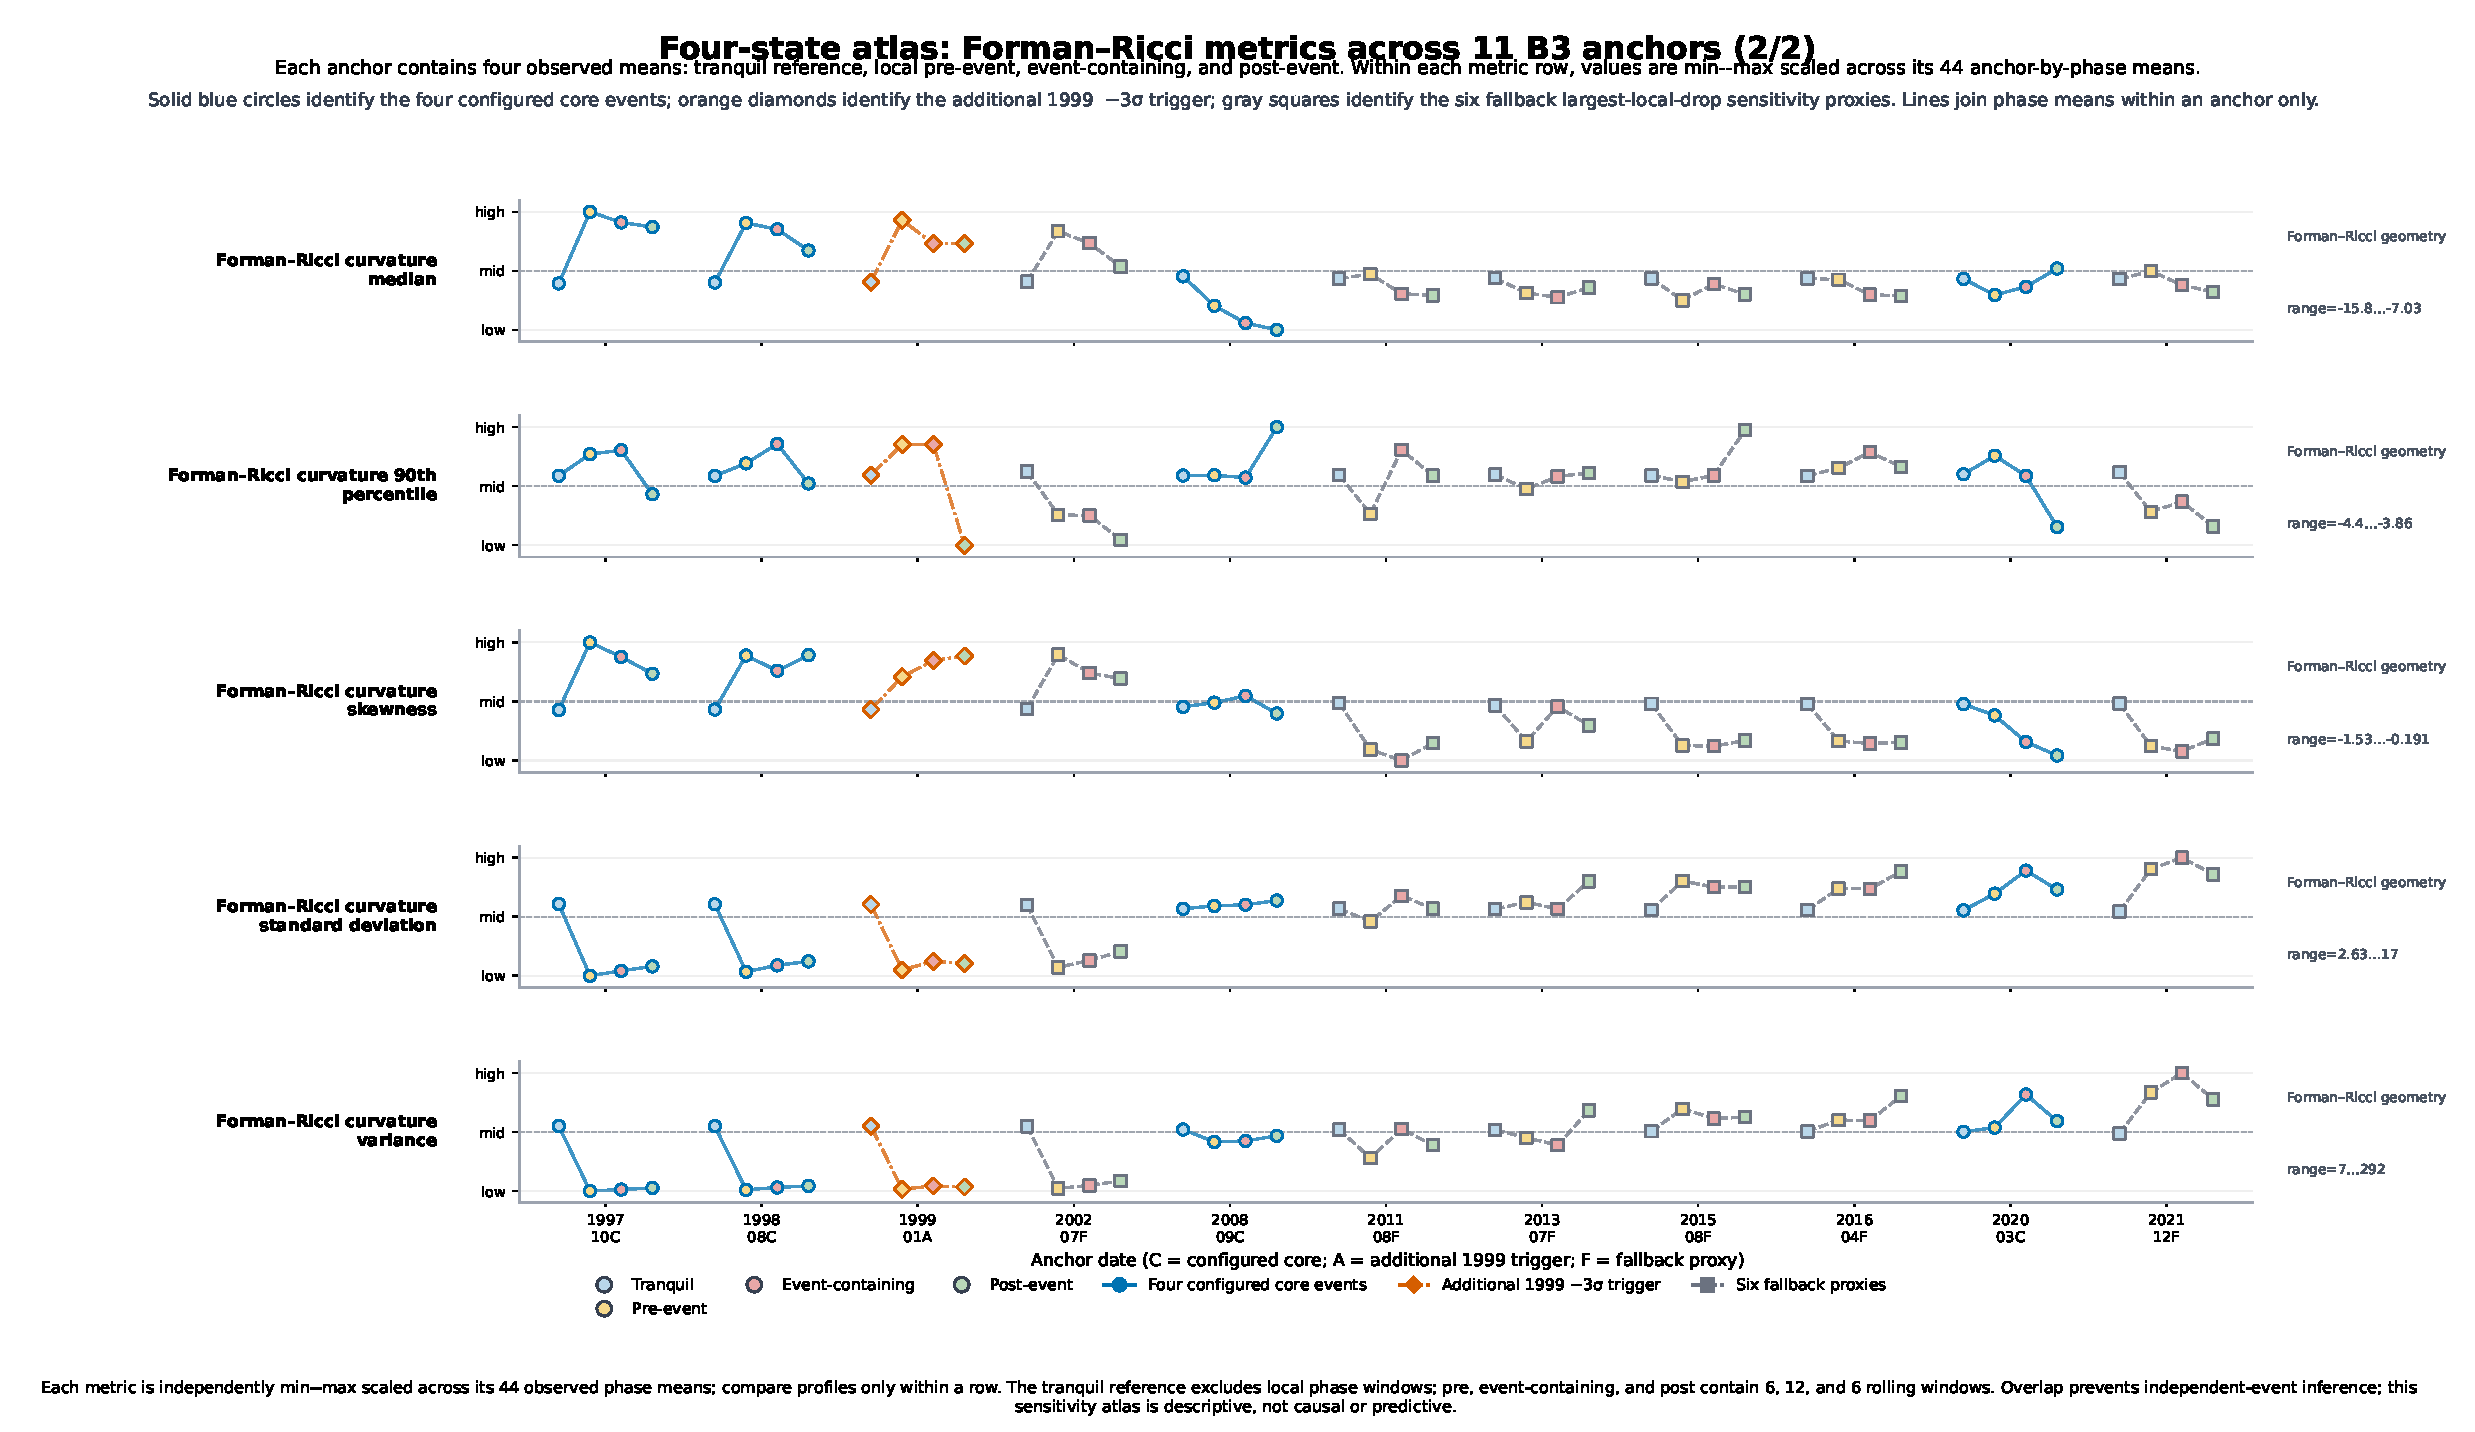
\includegraphics[width=0.90\textheight,height=0.86\textwidth,keepaspectratio]{figures/validation/proxy_11_ricci_metric_contrasts_part2.pdf}
\caption[]{Four-state sensitivity atlas (continued): remaining five Forman--Ricci metrics.}
\end{sidewaysfigure}

As a sensitivity check, the expanded proxy calendar preserves the broadest distance and matrix-validation contrasts in the four configured core events. Relative to the local pre-event phase, PMFG mean distance decreases, whereas distance variance, the KS Gaussian-null statistic, the MP signal-variance fraction, and the MP market-mode fraction increase in all four core events. The additional 1999 trigger and the six fallback anchors show more heterogeneous agreement, particularly for mesoscopic and size-conditioned centrality diagnostics. Figure~\ref{fig:proxy-11-non-ricci} summarizes these contrasts across the 11-anchor calendar; because each metric row is independently scaled, the atlas is a visual profile comparison rather than a pooled effect-size estimate.

Table~\ref{tab:phase-concordance} gives the complete 13-metric concordance matrix across the four configured core events, the additional 1999 $-3\sigma$ trigger, and the six fallback anchors. Table~\ref{tab:anchor-context} complements it with the observed shock magnitude, drawdown, duration, and recovery for every anchor. Together, these tables make the central distinction explicit: the core-event subset shows the strongest and most coherent distance--spectral configuration, whereas the additional trigger and fallback proxies retain more heterogeneous mesoscopic and centrality responses. This heterogeneity is informative because it helps distinguish system-level stress configurations from routine local declines under the same descriptive protocol.

\begin{table}[width=\textwidth,pos=h]
\centering
\caption{Phase-concordance of the 13-metric core panel relative to local pre-event means. Signs indicate the dominant direction and the number of anchors with that direction. Distance moments and modularity are raw descriptive context; group and centrality measures are size-conditioned residuals. ``Mixed'' denotes no directional majority.}
\label{tab:phase-concordance}
\scriptsize
\setlength{\tabcolsep}{3pt}
\renewcommand{\arraystretch}{1.12}
\begin{tabular*}{\tblwidth}{@{}llcccccc@{}}
\toprule
& & \multicolumn{2}{c}{Configured events ($n=4$)} & \multicolumn{2}{c}{Actual $-3\sigma$ triggers ($n=5$)} & \multicolumn{2}{c}{Fallback anchors ($n=6$)} \\
\cmidrule(lr){3-4}\cmidrule(lr){5-6}\cmidrule(l){7-8}
Family & Metric & During--pre & Post--pre & During--pre & Post--pre & During--pre & Post--pre \\
\midrule
Distance & Mean & $-\;(4/4)$ & $-\;(4/4)$ & $-\;(5/5)$ & $-\;(4/5)$ & $-\;(4/6)$ & $-\;(4/6)$ \\
(raw context) & Variance & $+\;(4/4)$ & $+\;(4/4)$ & $+\;(5/5)$ & $+\;(4/5)$ & mixed & $-\;(4/6)$ \\
& Skewness & $+\;(4/4)$ & $+\;(3/4)$ & $+\;(5/5)$ & $+\;(3/5)$ & $+\;(4/6)$ & $+\;(4/6)$ \\
& Kurtosis & $-\;(3/4)$ & $-\;(3/4)$ & $-\;(3/5)$ & $-\;(3/5)$ & $-\;(4/6)$ & $-\;(5/6)$ \\
\midrule
Mesoscopic & PMFG modularity (raw) & $+\;(3/4)$ & $+\;(4/4)$ & $+\;(4/5)$ & $+\;(5/5)$ & mixed & $-\;(4/6)$ \\
& PMFG community residual & mixed & $-\;(3/4)$ & $+\;(3/5)$ & $-\;(3/5)$ & $-\;(4/6)$ & $+\;(4/6)$ \\
& Ward group residual & $+\;(3/4)$ & $+\;(3/4)$ & $+\;(4/5)$ & $+\;(4/5)$ & $+\;(5/6)$ & $+\;(6/6)$ \\
\midrule
Centrality & Betweenness residual & $+\;(3/4)$ & mixed & $+\;(4/5)$ & $+\;(3/5)$ & $+\;(4/6)$ & $-\;(4/6)$ \\
(size-adjusted) & Closeness residual & mixed & $-\;(3/4)$ & $-\;(3/5)$ & $-\;(4/5)$ & mixed & $+\;(4/6)$ \\
& Eigenvector residual & mixed & mixed & $-\;(3/5)$ & $-\;(3/5)$ & $+\;(4/6)$ & $+\;(4/6)$ \\
\midrule
Matrix & KS statistic & $+\;(4/4)$ & $+\;(3/4)$ & $+\;(5/5)$ & $+\;(3/5)$ & $+\;(5/6)$ & $+\;(5/6)$ \\
validation & MP signal fraction & $+\;(4/4)$ & $+\;(4/4)$ & $+\;(5/5)$ & $+\;(4/5)$ & mixed & $+\;(4/6)$ \\
& MP market-mode fraction & $+\;(4/4)$ & $+\;(3/4)$ & $+\;(5/5)$ & $+\;(3/5)$ & $+\;(4/6)$ & mixed \\
\bottomrule
\end{tabular*}
\end{table}


\begin{table}[width=\textwidth,pos=h]
\centering
\caption{Observed anchor context and phase-transition summary. ``International named shock'' identifies a pre-specified core anchor with an established international crisis label; ``B3-local proxy'' denotes the observed B3 decline selected by the sensitivity rule, not a causal attribution. Shock return is the daily B3 return at the selected shock date. Drawdown, duration, and recovery are descriptive properties of the local price path.}
\label{tab:anchor-context}
\scriptsize
\setlength{\tabcolsep}{3.5pt}
\renewcommand{\arraystretch}{1.10}
\begin{tabular*}{\tblwidth}{@{}lllrrrrl@{}}
\toprule
Anchor & Observed context & Status & Shock & $z$ & Drawdown & Days & Recovery \\
\midrule
1997-10-27 & International named shock: Asian crisis & $-3\sigma$ trigger; core & $-11.56\%$ & $-4.44$ & $-71.94\%$ & 753 & yes \\
1998-08-27 & International named shock: Russian default/LTCM & $-3\sigma$ trigger; core & $-8.44\%$ & $-3.24$ & $-34.82\%$ & 88 & yes \\
1999-01-13 & Additional B3 $-3\sigma$ trigger & $-3\sigma$ trigger & $-11.28\%$ & $-4.33$ & $-20.70\%$ & 6 & yes \\
2002-07-22 & B3-local proxy & fallback local drop & $-7.40\%$ & $-2.84$ & $-15.76\%$ & 37 & yes \\
2008-09-29 & International named shock: global financial crisis & $-3\sigma$ trigger; core & $-8.74\%$ & $-3.36$ & $-40.16\%$ & 242 & yes \\
2011-08-08 & B3-local proxy & fallback local drop & $-7.45\%$ & $-2.86$ & $-7.18\%$ & 3 & yes \\
2013-07-02 & B3-local proxy & fallback local drop & $-4.62\%$ & $-1.77$ & $-6.51\%$ & 20 & yes \\
2015-08-24 & B3-local proxy & fallback local drop & $-4.78\%$ & $-1.83$ & $-4.67\%$ & 3 & yes \\
2016-04-04 & B3-local proxy & fallback local drop & $-4.68\%$ & $-1.79$ & $-5.10\%$ & 8 & yes \\
2020-03-09 & International named shock: COVID-19 & $-3\sigma$ trigger; core & $-12.54\%$ & $-4.82$ & $-39.81\%$ & 121 & yes \\
2021-12-20 & B3-local proxy (2022 anchor) & fallback local drop & $-5.13\%$ & $-1.97$ & $-35.81\%$ & -- & no \\
\bottomrule
\end{tabular*}
\end{table}



The atlas confirms visually that the four configured core events share the strongest distance--spectral profile, while the additional 1999 trigger and six fallback anchors display greater heterogeneity. This is the appropriate level of interpretation for independently scaled rows: the figure documents recurrent configurations and metric-specific departures, but does not provide a pooled estimate or a forecast.

\subsection{Within-Pre-Event Trajectory Patterns}
\label{subsec:within-pre-trajectories}

The pre-event state can be resolved into six constituent rolling windows for every sensitivity anchor. The final within-pre-event step rises in the size-conditioned closeness residual in 10/11 anchors (5/5 actual triggers), in KS displacement in 9/11, and in distance variance, MP signal fraction, and market-mode fraction in 8/11; raw PMFG modularity falls in 7/11. These alignments concern only the explicitly defined fifth-to-sixth pre-window difference and do not establish a common precursor trajectory. Figure~\ref{fig:proxy-11-pre-trajectories} displays the complete 25-metric trajectory atlas in three consecutive panels.

\begin{center}
\captionsetup{type=figure}
\centering
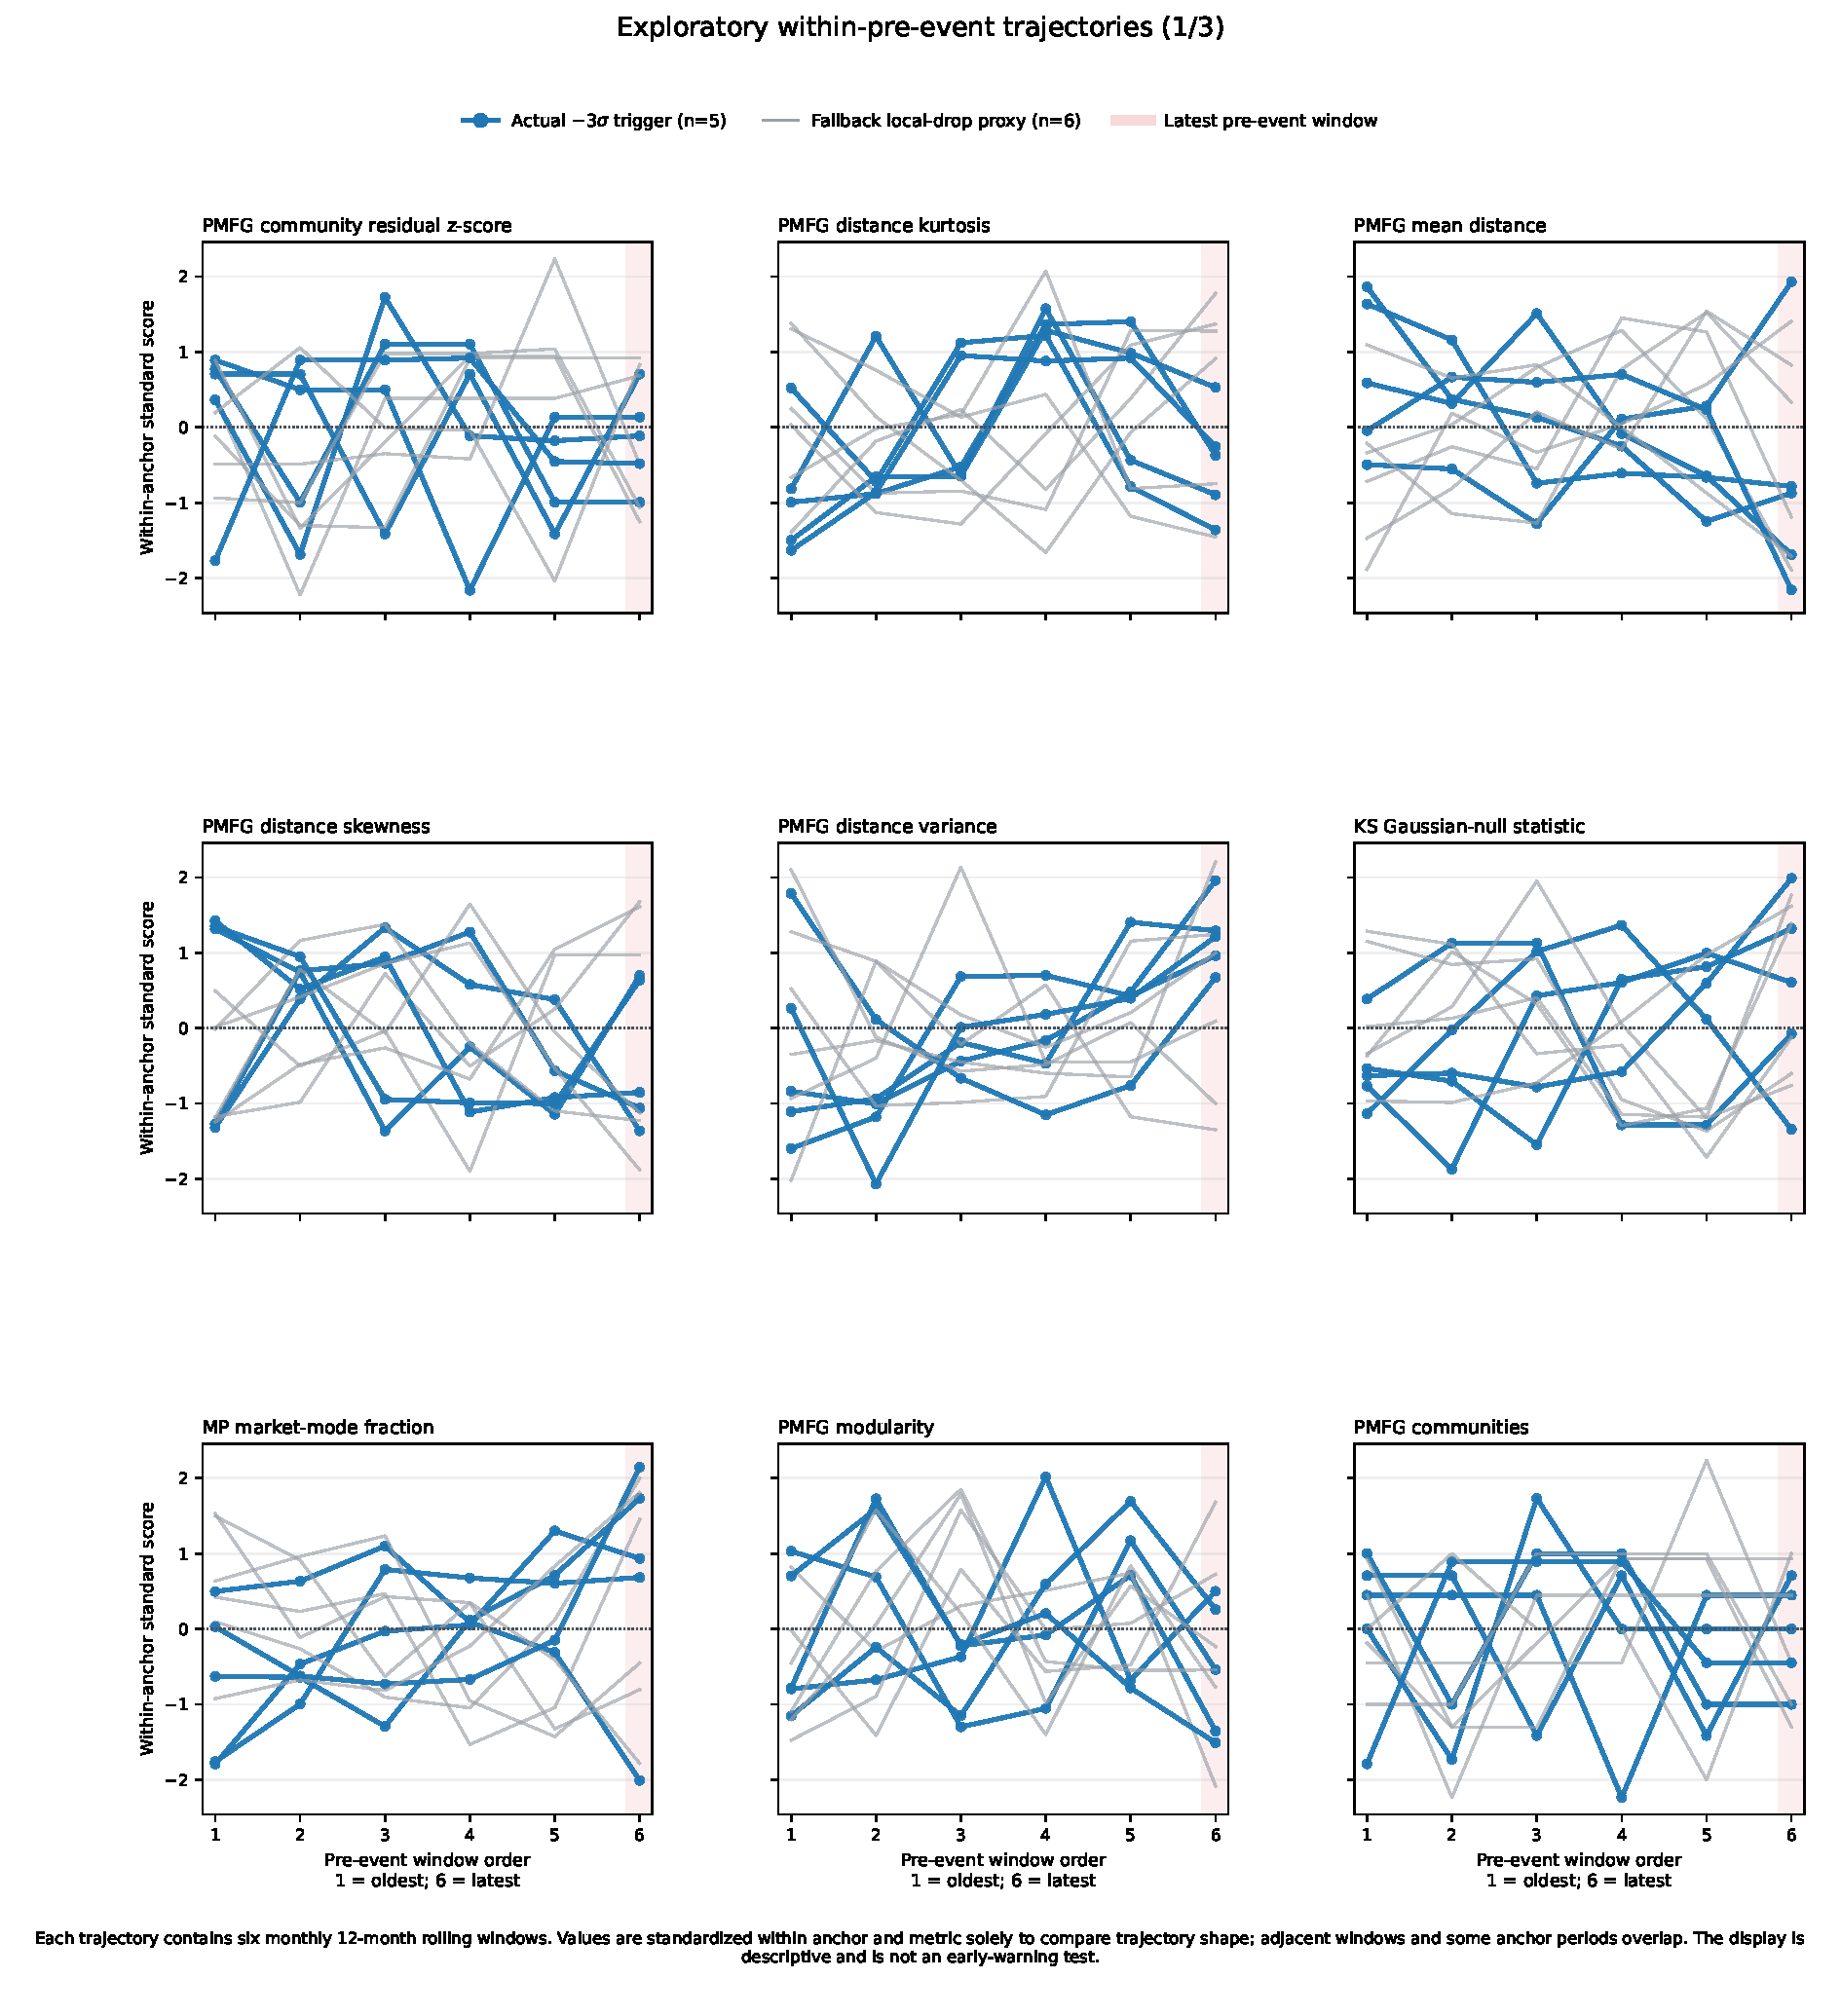
\includegraphics[width=0.98\linewidth,height=0.68\textheight,keepaspectratio]{figures/validation/proxy_11_pre_event_trajectories_part1.pdf}
\caption{Exploratory six-window pre-event trajectories for the first nine metrics across the 11-anchor B3 sensitivity calendar. Values are standardized within anchor and metric; blue and grey markers distinguish actual triggers from fallback proxies. Overlapping windows make this a descriptive display, not evidence of causality or prediction.}
\label{fig:proxy-11-pre-trajectories}
\end{center}

\begin{center}
\captionsetup{type=figure}
\ContinuedFloat
\centering
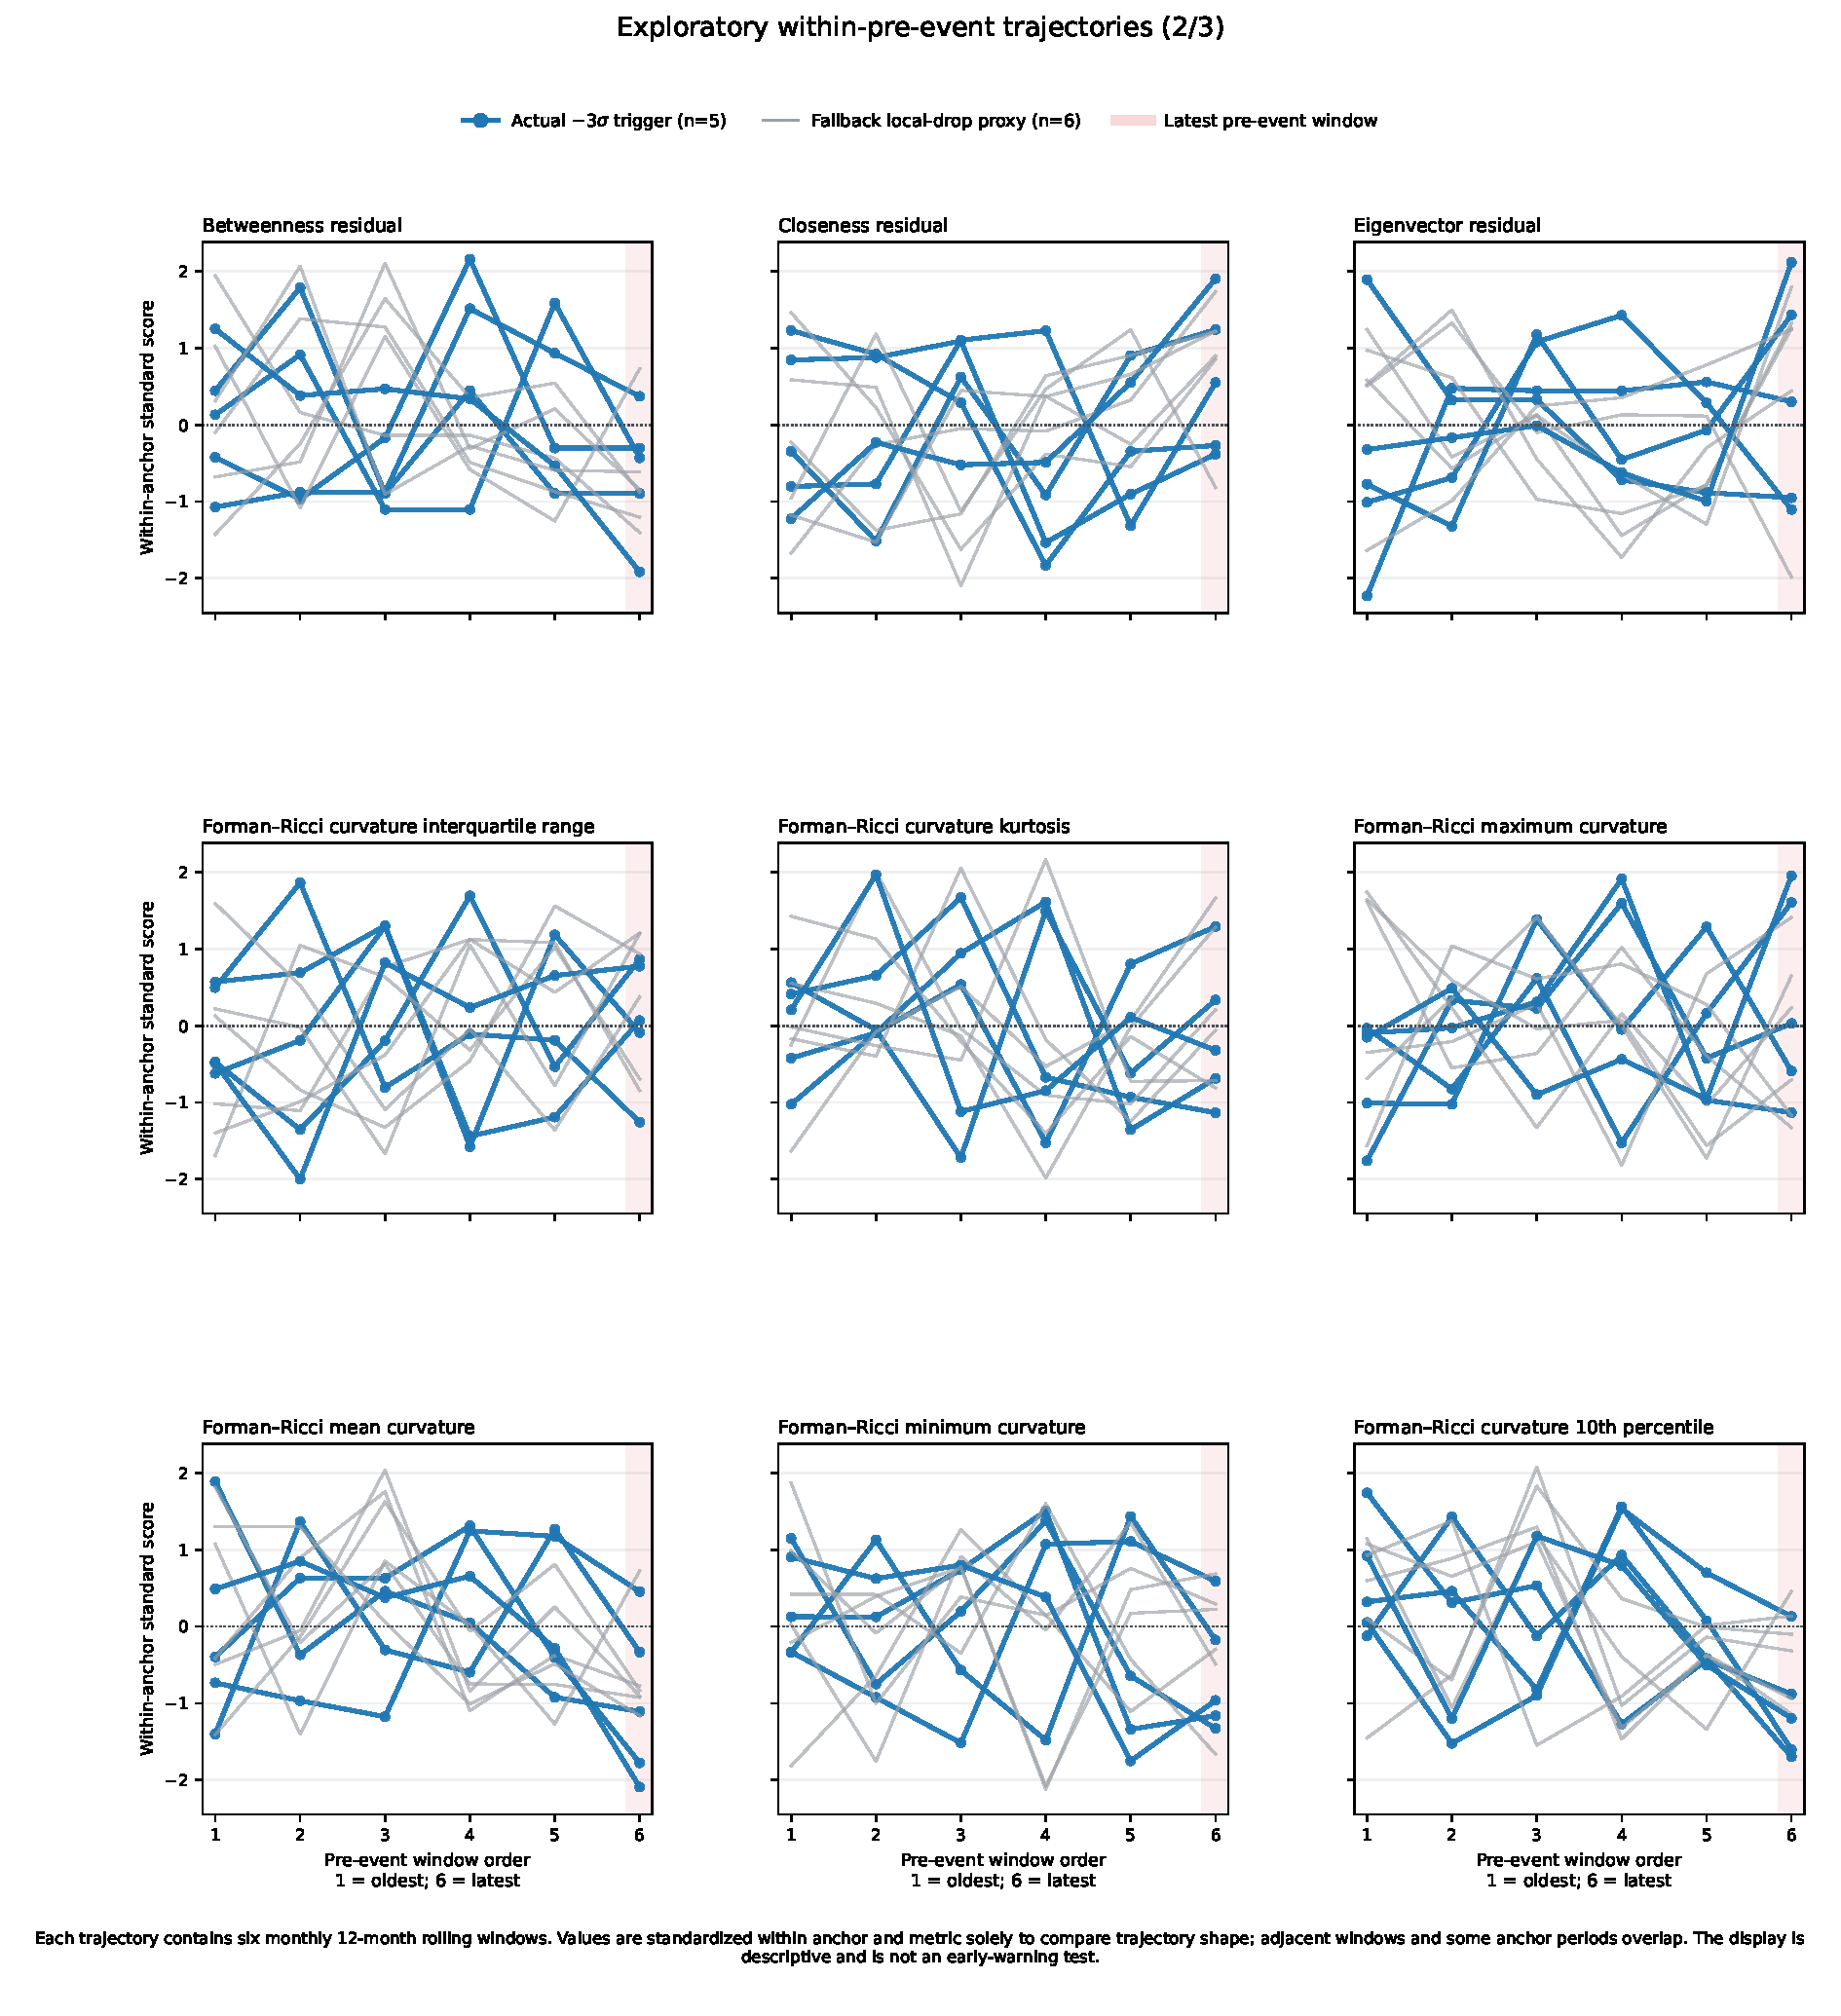
\includegraphics[width=0.98\linewidth,height=0.68\textheight,keepaspectratio]{figures/validation/proxy_11_pre_event_trajectories_part2.pdf}
\caption[]{Exploratory six-window pre-event trajectories (continued): metrics 10--18.}
\end{center}

\begin{center}
\captionsetup{type=figure}
\ContinuedFloat
\centering
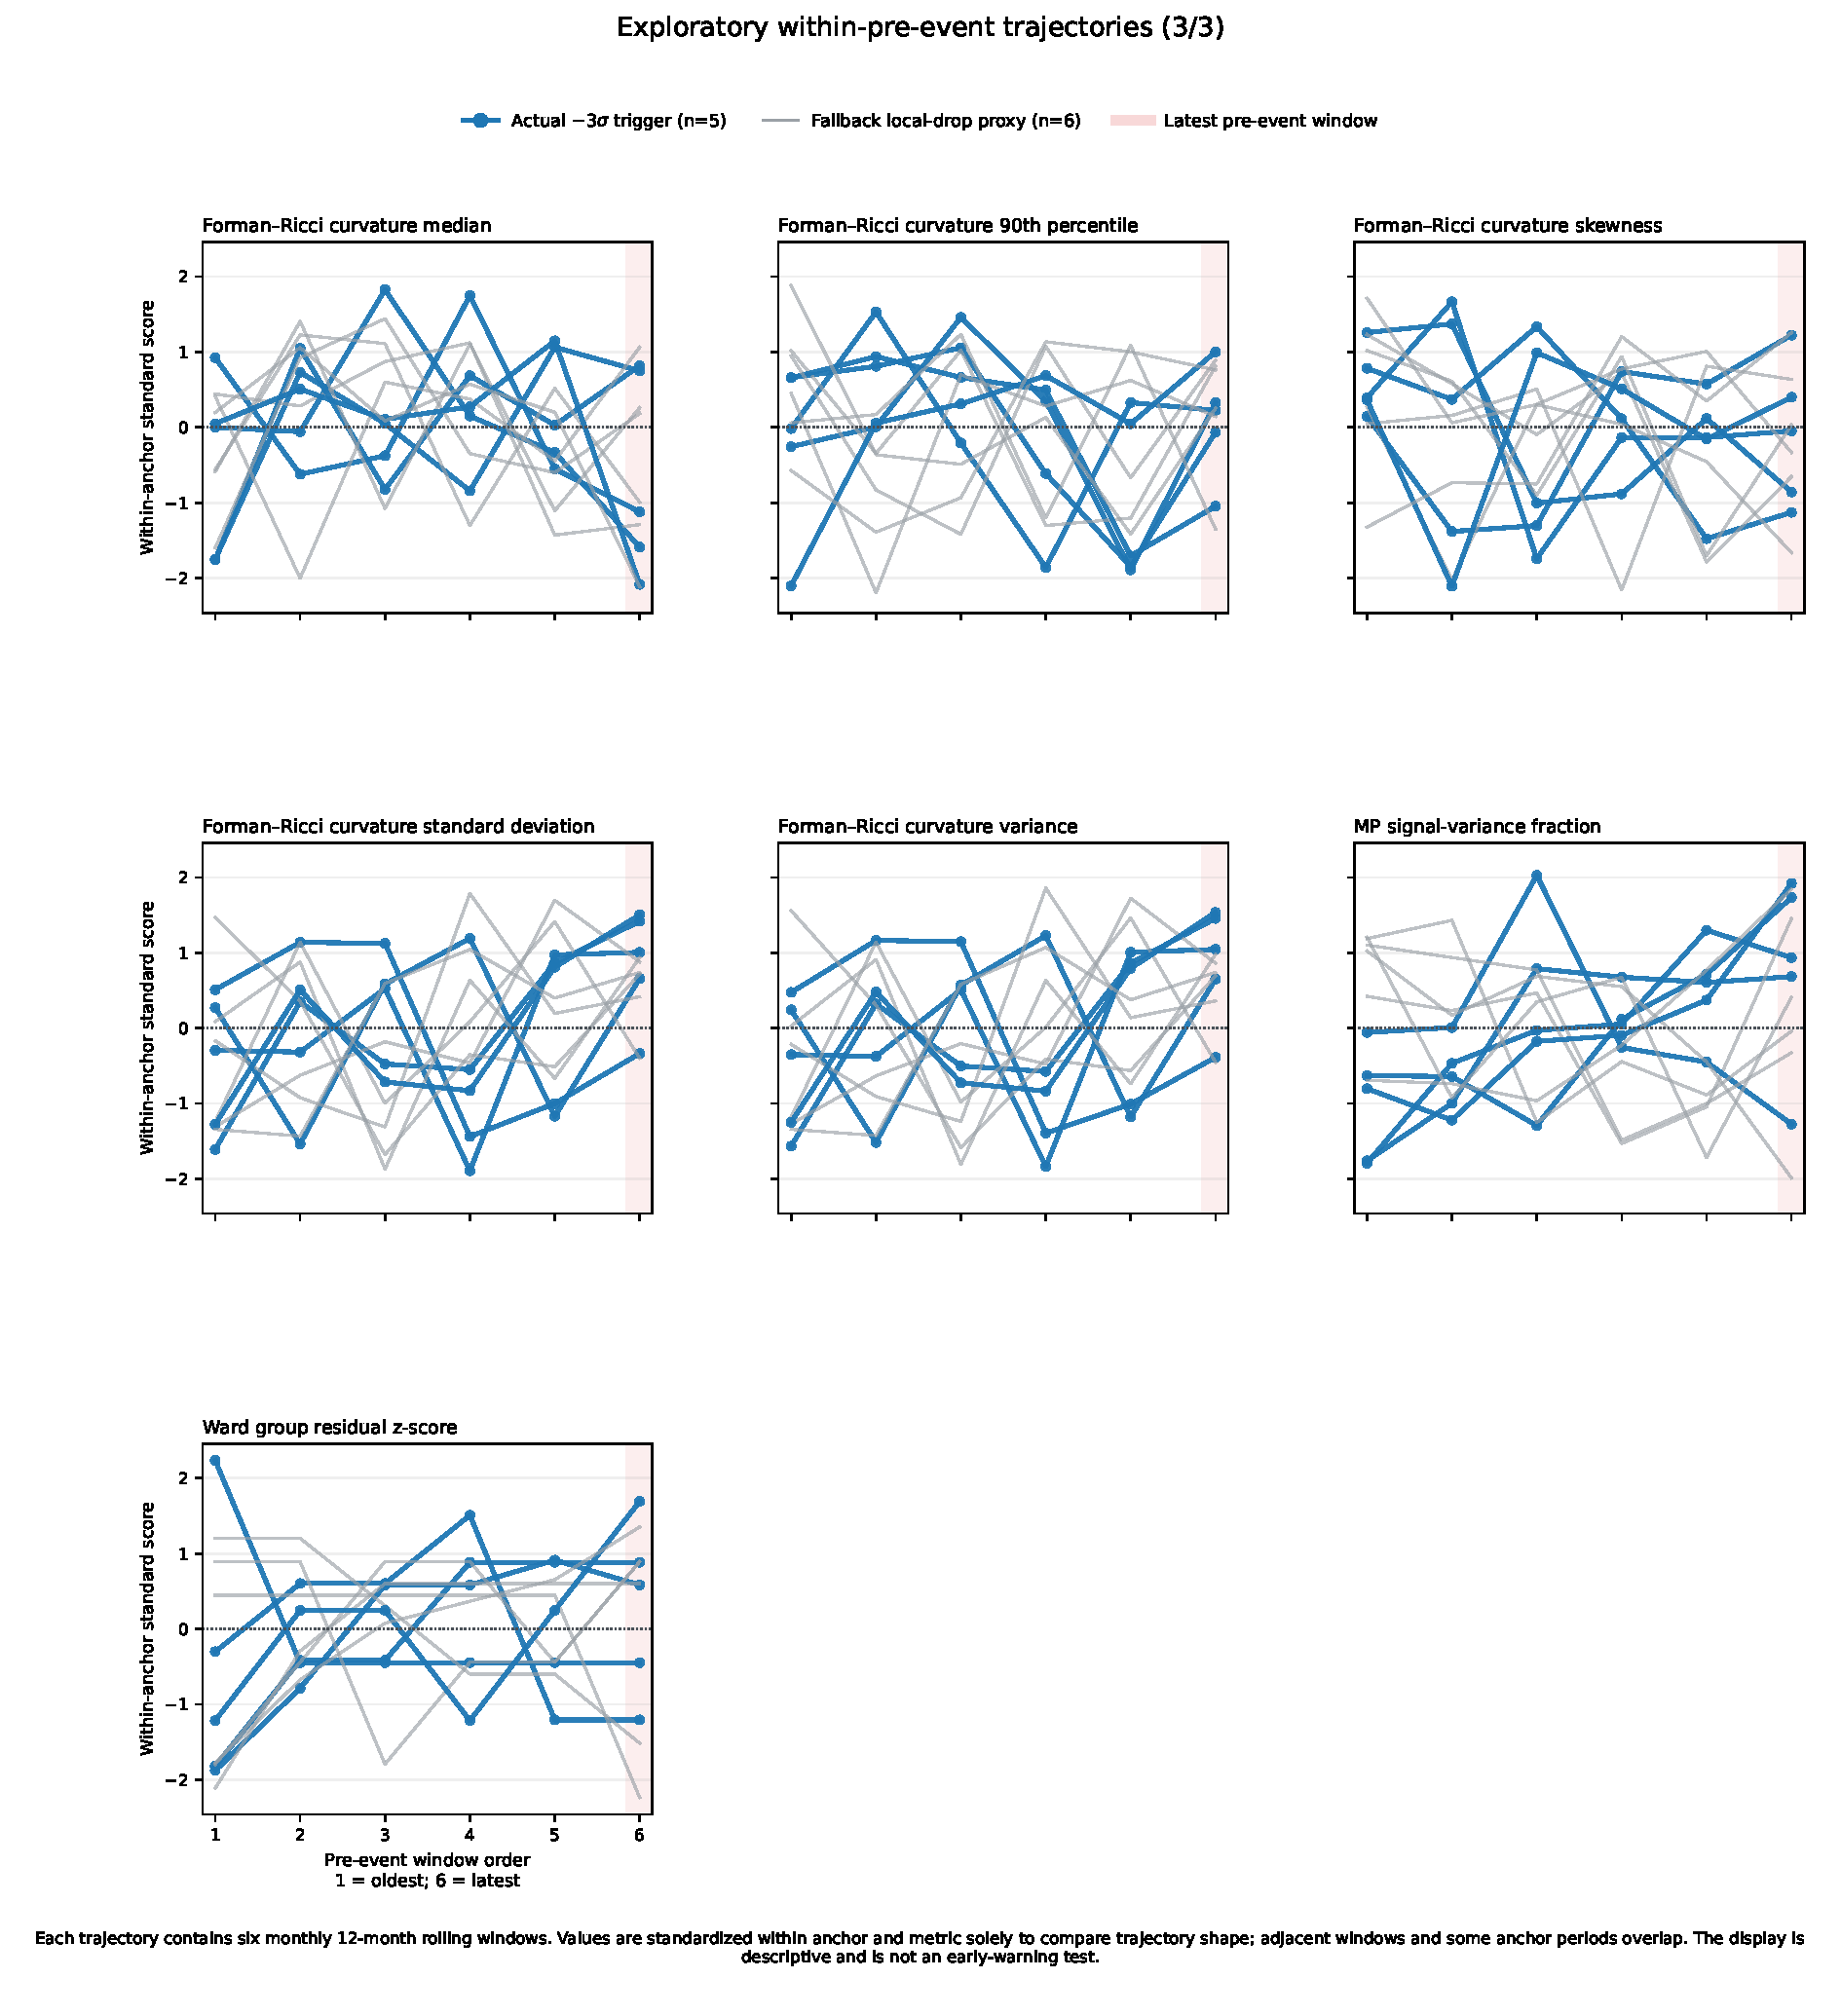
\includegraphics[width=0.98\linewidth,height=0.68\textheight,keepaspectratio]{figures/validation/proxy_11_pre_event_trajectories_part3.pdf}
\caption[]{Exploratory six-window pre-event trajectories (continued): metrics 19--25.}
\end{center}

The trajectory atlas should be read row by row and anchor by anchor. Standardization makes the direction and shape of each local path visible, but removes cross-metric level information; overlapping windows also prevent the lines from being treated as independent observations. The figure is therefore useful for documenting within-pre-event alignments while remaining unsuitable as an early-warning test. In particular, the visual paths are descriptive within-anchor trajectories, not evidence that any metric anticipates or causes stress.

\begin{table}[!t]
\centering
\caption{Two local-pre-referenced contrasts derived from the four-state phase protocol across the four configured events. Signs indicate the dominant direction and the number of configured events with that direction. Tranquil and phase-level means are displayed separately in Figure~\ref{fig:four-state-crisis-infographic}. Distance moments and modularity are raw descriptive context; group and centrality measures are size-conditioned residuals. ``Mixed'' denotes no directional majority.}
\label{tab:phase-concordance-core}
\scriptsize
\setlength{\tabcolsep}{5pt}
\renewcommand{\arraystretch}{0.88}
\begin{tabular*}{\linewidth}{@{\extracolsep{\fill}}llcc@{}}
\toprule
Family & Metric & During--pre & Post--pre \\
\midrule
Distance & Mean & $-\;(4/4)$ & $-\;(4/4)$ \\
(raw context) & Variance & $+\;(4/4)$ & $+\;(4/4)$ \\
& Skewness & $+\;(4/4)$ & $+\;(3/4)$ \\
& Kurtosis & $-\;(3/4)$ & $-\;(3/4)$ \\
\midrule
Mesoscopic & PMFG modularity (raw) & $+\;(3/4)$ & $+\;(4/4)$ \\
& PMFG community residual & mixed & $-\;(3/4)$ \\
& Ward group residual & $+\;(3/4)$ & $+\;(3/4)$ \\
\midrule
Centrality & Betweenness residual & $+\;(3/4)$ & mixed \\
(size-adjusted) & Closeness residual & mixed & $-\;(3/4)$ \\
& Eigenvector residual & mixed & mixed \\
\midrule
Matrix & KS statistic & $+\;(4/4)$ & $+\;(3/4)$ \\
validation & MP signal fraction & $+\;(4/4)$ & $+\;(4/4)$ \\
& MP market-mode fraction & $+\;(4/4)$ & $+\;(3/4)$ \\
\bottomrule
\end{tabular*}
\end{table}

The transition from pre to event-containing windows is the most reproducible structural transition. Across the four configured events, it combines lower mean PMFG distance with higher distance variance and skewness, KS displacement, MP signal fraction, and MP market-mode fraction in 4/4 cases. Distance kurtosis is lower in 3/4 configured events, whereas the size-conditioned eigenvector-centrality residual is mixed (two increases and two decreases), despite its relevance as a hub-concentration diagnostic \citep{bonacich1987power}.

As an ancillary check, the pipeline's pooled constituent-return volatility statistic is higher in event-containing than in local pre-event windows for the 1997, 1998, and 2020 anchors, but slightly lower for 2008. This statistic is the within-window dispersion of pooled constituent log returns, not an IBOVESPA-index volatility series; it therefore provides qualified context rather than a universal volatility transition.

The post phase represents a partial rather than uniform continuation of the event-containing configuration. For the four configured anchors, lower mean distance and higher distance variance and MP signal fraction persist in 4/4 comparisons; KS displacement, distance skewness, and the MP market-mode fraction persist in 3/4. Lower distance kurtosis also persists in 3/4, while the eigenvector-centrality residual remains mixed across configured events. Modularity, group residuals, and centralities do not provide a universal transition path. The evidence therefore supports a descriptive sequence of a mixed pre-state, a recurrent distance--spectral reconfiguration during stress, and heterogeneous post-event reorganization; it does not identify a common causal mechanism or an early-warning trajectory.

For the 11-anchor sensitivity calendar, KS displacement and the MP signal fraction recur in the during/pre comparison within the actual-trigger subset, whereas mesoscopic patterns remain heterogeneous. A two-profile clustering of the structural summaries has weak separation (silhouette $=0.251$); only the 1997 and 2020 anchors are assigned to profile 2. The observed association between profile membership and anchor severity/duration is descriptive only and does not support inference about historical mechanisms.

The structural-profile calculation provides a final numerical sensitivity check. Its weak separation and small membership of the second profile support only a descriptive grouping of anchors; they do not identify mechanisms, stable regimes, or a transferable classification rule.

\section{Discussion}
\label{sec:discussion}

The discussion is organized as a descriptive regime taxonomy rather than a causal-role classification. For each documented event, the core design uses a tranquil benchmark and three local phases: pre-crisis windows, windows containing the event date, and post-crisis windows. Raw distance moments and modularity provide geometric context, whereas group and centrality residuals identify deviations from the empirical size-only expectation. Thus, the local phase contrasts do not establish temporal causality, out-of-sample prediction, or a universal ordering of indicators.

The resulting picture is heterogeneous rather than a uniform collapse. Size-adjusted distance metrics, Ward group residuals, PMFG communities, centralities, and KS/MP diagnostics provide complementary descriptions of reorganization. The appropriate practical use is comparative monitoring: a window can be located within a historical tranquil/pre-crisis/during/post-crisis taxonomy, but no individual diagnostic is promoted as a causal early-warning signal.

The expanded visual evidence is consistent with this qualified interpretation. The non-curvature atlas, Forman--Ricci atlas, and six-window pre-event trajectories in Figures~\ref{fig:proxy-11-non-ricci}--\ref{fig:proxy-11-pre-trajectories} make the recurring distance--spectral configuration visible while retaining the heterogeneity of mesoscopic and centrality responses across the 11-anchor calendar. These displays are exploratory within-anchor evidence; they do not establish a common precursor, causal mechanism, or predictive signal. The weak profile separation is retained numerically in the sensitivity discussion rather than as a separate figure.

% -----------------------------------------------------------------------
% -----------------------------------------------------------------------
\subsection{Synthesis: Were the Objectives Met? Contributions, Limitations, and Future Work}
\label{sec:synthesis}
% -----------------------------------------------------------------------

\paragraph{Research objectives and the problem statement.}


The paper evaluates whether a planar-first rolling pipeline can document size-conditioned structural configurations around a pre-specified B3 stress calendar. The evidence supports this descriptive objective: tranquil, pre-crisis, event-containing, and post-crisis windows differ as joint configurations, with KS/MP changes recurring across all four events and mesoscopic diagnostics documenting their event-level heterogeneity.

\paragraph{Key contributions.}


The paper makes four operational and substantive contributions. First, it documents a reproducible planar-first pipeline for rolling B3 network diagnostics. Second, it conditions reported cross-window comparisons on the eligible asset-universe size. Third, it evaluates every reported diagnostic family across all four configured severe drawdowns. Fourth, it demonstrates that structural reconfiguration is a joint, episode-specific configuration rather than a universal movement in one variable.

\paragraph{Methodological caveats and scope limitations.}

Two main limitations qualify the results and scope of the findings. First, rolling windows with fixed length $W = 252$ days inevitably smooth rapid events. The March 2020 crash unfolded over a few weeks; the window surrounding it captures the before-and-after but loses the intraweek timing precision that event-study methods would provide. This limits temporal localization, rather than the descriptive comparison of configurations. Second, the Pearson correlation estimator is sensitive to outliers and non-Gaussian tails. While the KS test confirms that empirical correlations are non-Gaussian relative to an i.i.d.\ Gaussian null, the estimator does not explicitly model tail dependence or volatility regime-switching, potentially underestimating co-dependence severity during stress periods. A copula-based or rank-correlation alternative could address this in future work.

\paragraph{Future work.}


Two extensions are most immediately valuable. (i)~\emph{Predictive evaluation}: use a separate out-of-sample design with ROC and precision--recall analysis. (ii)~\emph{Alternative dependence measures}: replace Pearson correlation with copula or tail-dependence estimators in acute stress windows.

\paragraph{Strengths of the study.}


The principal strength of the study is its transparent delimitation of the evidence: the pipeline distinguishes a tranquil benchmark from pre-event, event-containing, and post-event configurations without claiming that any metric anticipates or causes stress. This makes the outputs suitable for exploratory historical comparison and for motivating subsequent confirmatory designs.

\paragraph{Limitations.}

Several limitations bound the scope of the conclusions. First, the study relies on daily adjusted closing prices and Pearson correlation as the dependency estimator; in acute stress periods, where return distributions become heavy-tailed and potentially non-elliptical, linear correlation may understate tail co-dependence. Replacing Pearson with rank-based or copula estimators in crisis windows is a direct methodological extension. Second, the crisis calendar is calibrated from historical accounts and market reports for the B3 context; the results are therefore sensitive to the chosen event set, and reasonable alternative event definitions could shift hit-rate rankings. Third, the sample is restricted to B3 equities with sufficient return history, which introduces survivorship and listing-vintage effects that are not explicitly controlled. Fourth, the framework is descriptive and retrospective: all results are in-sample, and no claim is made about real-time predictive performance. Out-of-sample evaluation under expanding-window or blocked cross-validation schemes remains an open and practically important extension. Fifth, the analysis focuses on the equity layer of the B3 universe; extending to fixed income, derivatives, or cross-border network layers could alter both the taxonomy of variables and the observed crisis signatures.

\section{Conclusion}
\label{sec:conclusion}


This paper develops a descriptive, planar-first reading of financial-network regimes in B3. The PMFG extracted from full rolling distance matrices is the main structural object, while heatmaps and dendrograms provide complementary visual context.

The all-event comparison identifies the event-containing configuration as lower mean PMFG distance and higher distance variance, distance skewness, KS displacement, MP signal fraction, and MP market-mode fraction in all four configured events. Post-event windows retain lower mean distance, higher distance variance, and higher MP signal fraction in all four comparisons. The planar and hierarchical layers add the essential mesoscopic detail: modularity, community and Ward-group measures, and centralities are partly concordant but remain event-specific. Thus, the empirical contribution is a joint regime taxonomy rather than a universal one-variable precursor. Mean PMFG degree is confirmed as a construction identity rather than a regime indicator.

These results are retrospective and descriptive. They support comparative historical monitoring across tranquil, pre-crisis, event-containing, and post-crisis configurations, but do not support causal, early-warning, or universal crisis claims.

\section*{Declaration of Generative AI and AI-assisted Technologies in the Writing Process}
During the preparation of this work, the authors used GitHub Copilot as a generative-AI assistant for code generation, data processing, figure production, and drafting and revising manuscript text. The authors designed the context architecture and prompt-engineering workflow used with the tool, critically reviewed and edited all AI-assisted outputs, and independently developed the research conceptualization, methodology, and interpretation, and approved the final manuscript. The authors take full responsibility for the content of the publication.

\section*{CRediT authorship contribution statement}
\textbf{Gerson Nassor Cardoso}: Conceptualization, Methodology, Software, Formal analysis, Data curation, Visualization, Writing -- original draft.
\textbf{Renato Cesar Sato}: Supervision, Validation, Writing -- review \& editing.

\section*{Declaration of competing interests}
The authors declare no competing financial interests directly related to this study. The corresponding author is professionally employed as a Data Scientist at Bradesco; however, Bradesco had no role in study design, data collection, analysis, interpretation, manuscript writing, or the decision to submit this article.

\section*{Role of the funding source}
This research did not receive any specific grant from funding agencies in the public, commercial, or not-for-profit sectors.

\section*{Data Availability}
The adjusted price data used to construct the rolling financial networks were retrieved from the official B3/BM\&FBovespa historical series (COTAHIST), distributed by Brasil, Bolsa Balc\~ao (B3) at \url{https://bvmf.bmfbovespa.com.br/InstDados/SerHist/}. The Paper 1 reproducibility code, configuration, figures, and selected derived outputs are available in the dedicated public repository at \url{https://github.com/gersonncardoso/taxonomy-critical-phenomena-financial-markets}; the complete derived-data archive is deposited in Zenodo at \url{https://doi.org/10.5281/zenodo.22037008}. The processed outputs are also available from the corresponding author upon reasonable request.

% Keep ordinary main-text figures near their citations. Only prevent any
% remaining float from crossing into the appendix boundary.
\FloatBarrier
\appendix
\numberwithin{figure}{section}
\numberwithin{table}{section}
\numberwithin{equation}{section}

\section{Figure Families and Supplementary Atlas}

For completeness, all generated figure families are integrated into the paper's interpretation through the following roles:
\begin{enumerate}
    \item Validation figures: rolling best-$k$, silhouette, modularity, KS and ADF summaries, and clustering sample tables.
    \item Hierarchical figures: first and last heatmaps and dendrograms, representing correlation-group formation and dissolution.
    \item Financial-network diagnostics: planar rolling metrics for modularity, communities, centralities, and distance moments.
    \item Representative network snapshots: first and last planar windows and the broader monthly atlas of filtered planar windows.
\end{enumerate}

The KDE is discussed in the main text as Figure~\ref{fig:distance-kde-3d}; Appendix~A retains the heatmap and dendrogram families as supplementary hierarchical context.

The supplementary heatmaps and dendrograms shown here use the Ward ordering
selected for the main hierarchical diagnostics. The pipeline also evaluates
average and complete linkage on the same rolling distance objects; their
comparative quality measures are reported in Appendix~C, Table~\ref{tab:method-comparison}.
The appendix figures are therefore boundary-window illustrations of the
selected hierarchy, not additional crisis claims. Their role is to show how
the correlation blocks and branch structure change at the sample boundaries
while the main text carries the rolling and event-level evidence.

\begin{center}
\captionsetup{type=figure}
\centering
\begin{subfigure}{\linewidth}
    \centering
    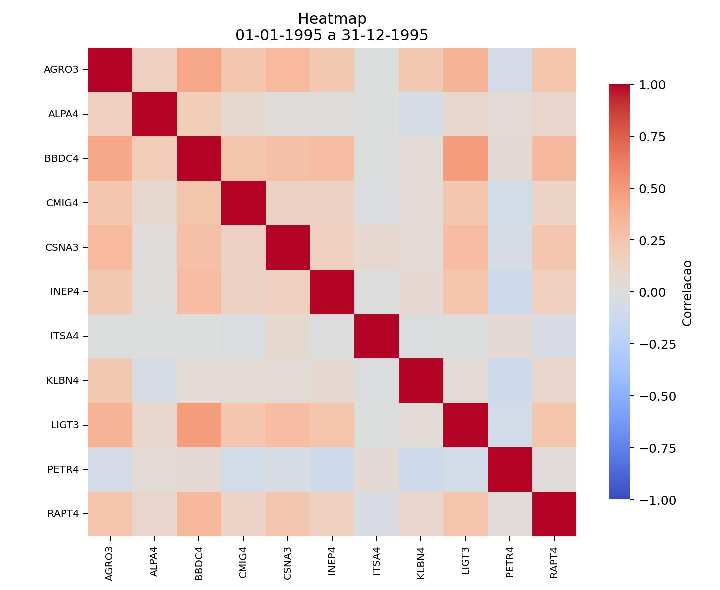
\includegraphics[width=\linewidth,height=0.38\textheight,keepaspectratio]{figures/heatmaps/heatmap_primeira_janela.pdf}
    \caption{Heatmap, first window.}
\end{subfigure}
\vspace{0.45em}
\begin{subfigure}{\linewidth}
    \centering
    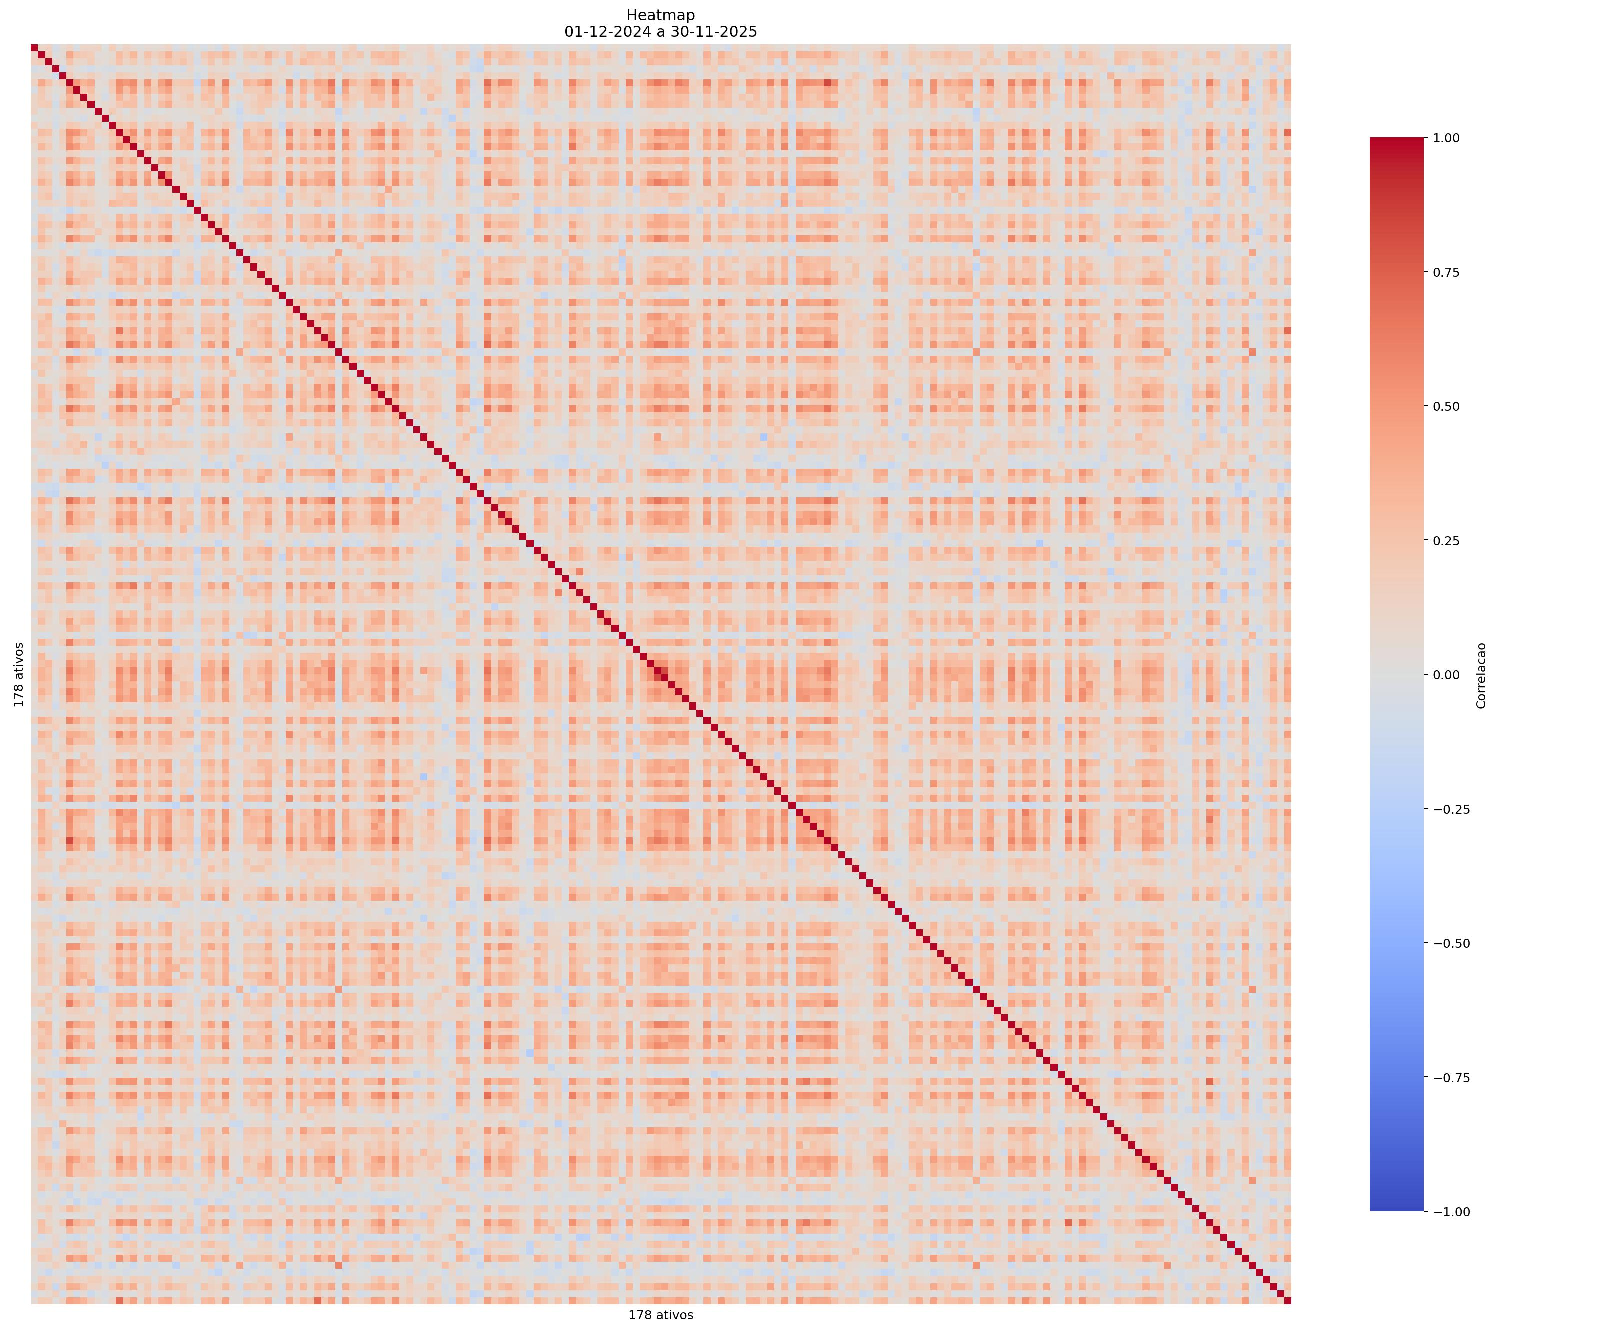
\includegraphics[width=\linewidth,height=0.38\textheight,keepaspectratio]{figures/heatmaps/heatmap_ultima_janela.pdf}
    \caption{Heatmap, last window.}
\end{subfigure}
\caption{Supplementary correlation heatmaps ordered by hierarchical clustering. The diagonal blocks summarize how correlation groups are organized at the beginning and end of the sample.}
\label{fig:heatmaps}
\end{center}

The heatmaps use the Ward ordering selected for the main hierarchical
diagnostics. The first-window panel is necessarily sparse because the eligible
universe is small at the beginning of the sample, whereas the last-window panel
contains a much larger cross-section. The visual comparison is therefore about
block organization and correlation mass, not about pixel-by-pixel density or
the raw number of colored cells. The changing universe is handled analytically
by the size-conditioned comparisons in the main text.

\begin{center}
\captionsetup{type=figure}
\centering
\begin{subfigure}{\linewidth}
    \centering
    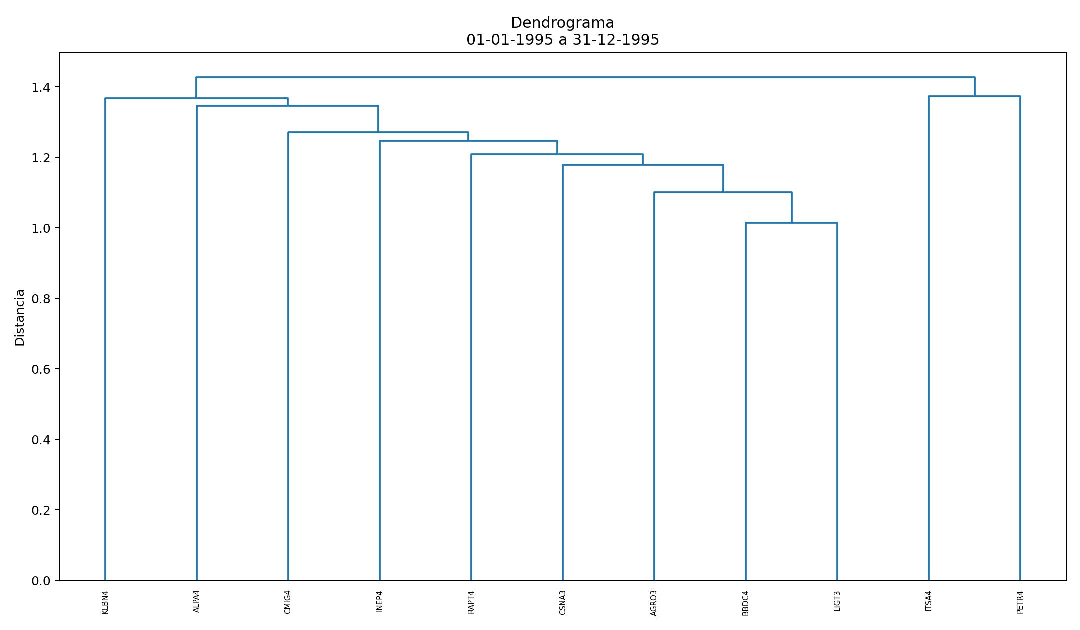
\includegraphics[width=\linewidth,height=0.36\textheight,keepaspectratio]{figures/dendrogramas/dendrograma_primeira_janela.pdf}
    \caption{Dendrogram, first window.}
\end{subfigure}
\vspace{0.45em}
\begin{subfigure}{\linewidth}
    \centering
    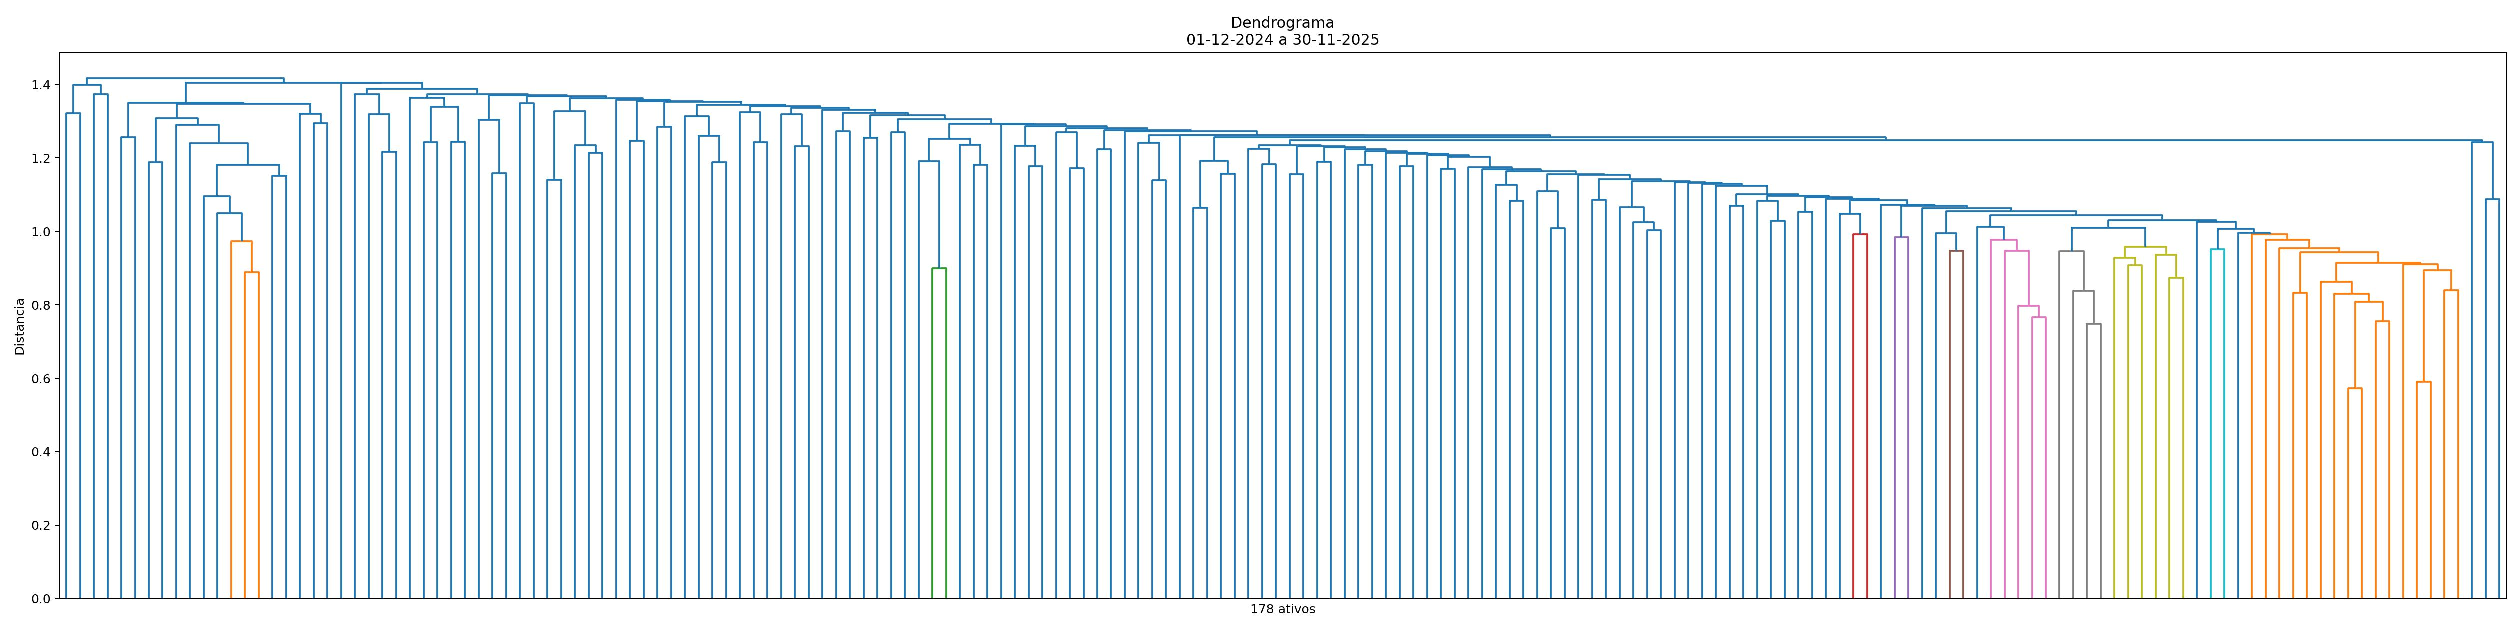
\includegraphics[width=\linewidth,height=0.36\textheight,keepaspectratio]{figures/dendrogramas/dendrograma_ultima_janela.pdf}
    \caption{Dendrogram, last window.}
\end{subfigure}
\caption{Supplementary Ward hierarchical clustering trees for the first and last rolling windows, constructed from the corresponding correlation-distance matrices. The comparison provides descriptive context for how the branching structure changes through time.}
\label{fig:dendrograms}
\end{center}

The dendrograms provide the complementary branch-level view. Ward linkage is
used for these boundary snapshots, while average and complete linkage remain
alternative methods evaluated in the representative comparison table. The
first-window tree has few leaves because only a limited number of assets meet
the historical eligibility rules; the last-window tree is denser because the
tradable universe has expanded. These panels document the visual consequence
of that expansion and are not treated as independent event-level evidence.

The monthly filtered-planar atlas should be interpreted as supplementary visual evidence supporting the aggregate rolling plots shown in the main text. The archive spans files \texttt{planar\_pval\_janela\_\{1,\dots,360\}.pdf}. It is too large to embed panel by panel in the article, but it is part of the documented empirical record and is explicitly incorporated as the window-by-window visual archive for the planar financial network.

\section{Portability Protocol --- Application to Other Equity, Credit, and Interbank Networks}

Although the present study uses Brazilian equity (B3) data, the framework is designed as a portable protocol that can be deployed to any financial network where rolling distance matrices can be constructed from multivariate time series. The protocol has three transferable components:

\begin{enumerate}
\item \textbf{Planar-first extraction}: Construct rolling Pearson distance matrices from asset returns; compute PMFG as the planar subgraph with maximum total edge weight; extract node-strength, distance-moment, and community-structure metrics. This step is agnostic to the underlying assets and can be applied to equities, bonds, foreign-exchange rates, or interbank credit exposures.

\item \textbf{Phase comparison}: Define crisis dates externally and compare tranquil, pre-crisis, event-containing, and post-crisis windows under the same size-conditioned measurement protocol. This design supports transparent historical comparison without assigning predictive roles to metrics.

\item \textbf{Multi-scale triangulation}: Compare hierarchical partitions, PMFG topology, distance moments, centralities, and spectral diagnostics. Use rolling windows of one year (or adjusted for the frequency of the data) with monthly updates and assign crisis events a priori using external documentation.

\end{enumerate}

To apply this protocol to an external dataset (e.g., S\&P 500 equities, euro-area bank credit networks, or foreign-exchange rate networks), follow these steps: (1) construct rolling distance matrices from asset returns or exposures; (2) compute PMFG subgraphs; (3) extract metrics; (4) identify crisis windows using external criteria; and (5) compare phase configurations under the same size-conditioned control. The code and pipeline are available from the authors upon request.

\section{Method-Comparison Clustering Diagnostics}

This appendix provides supplementary validation material that is not required for the main event-level interpretation.

\begin{center}
\captionsetup{type=figure}
\centering
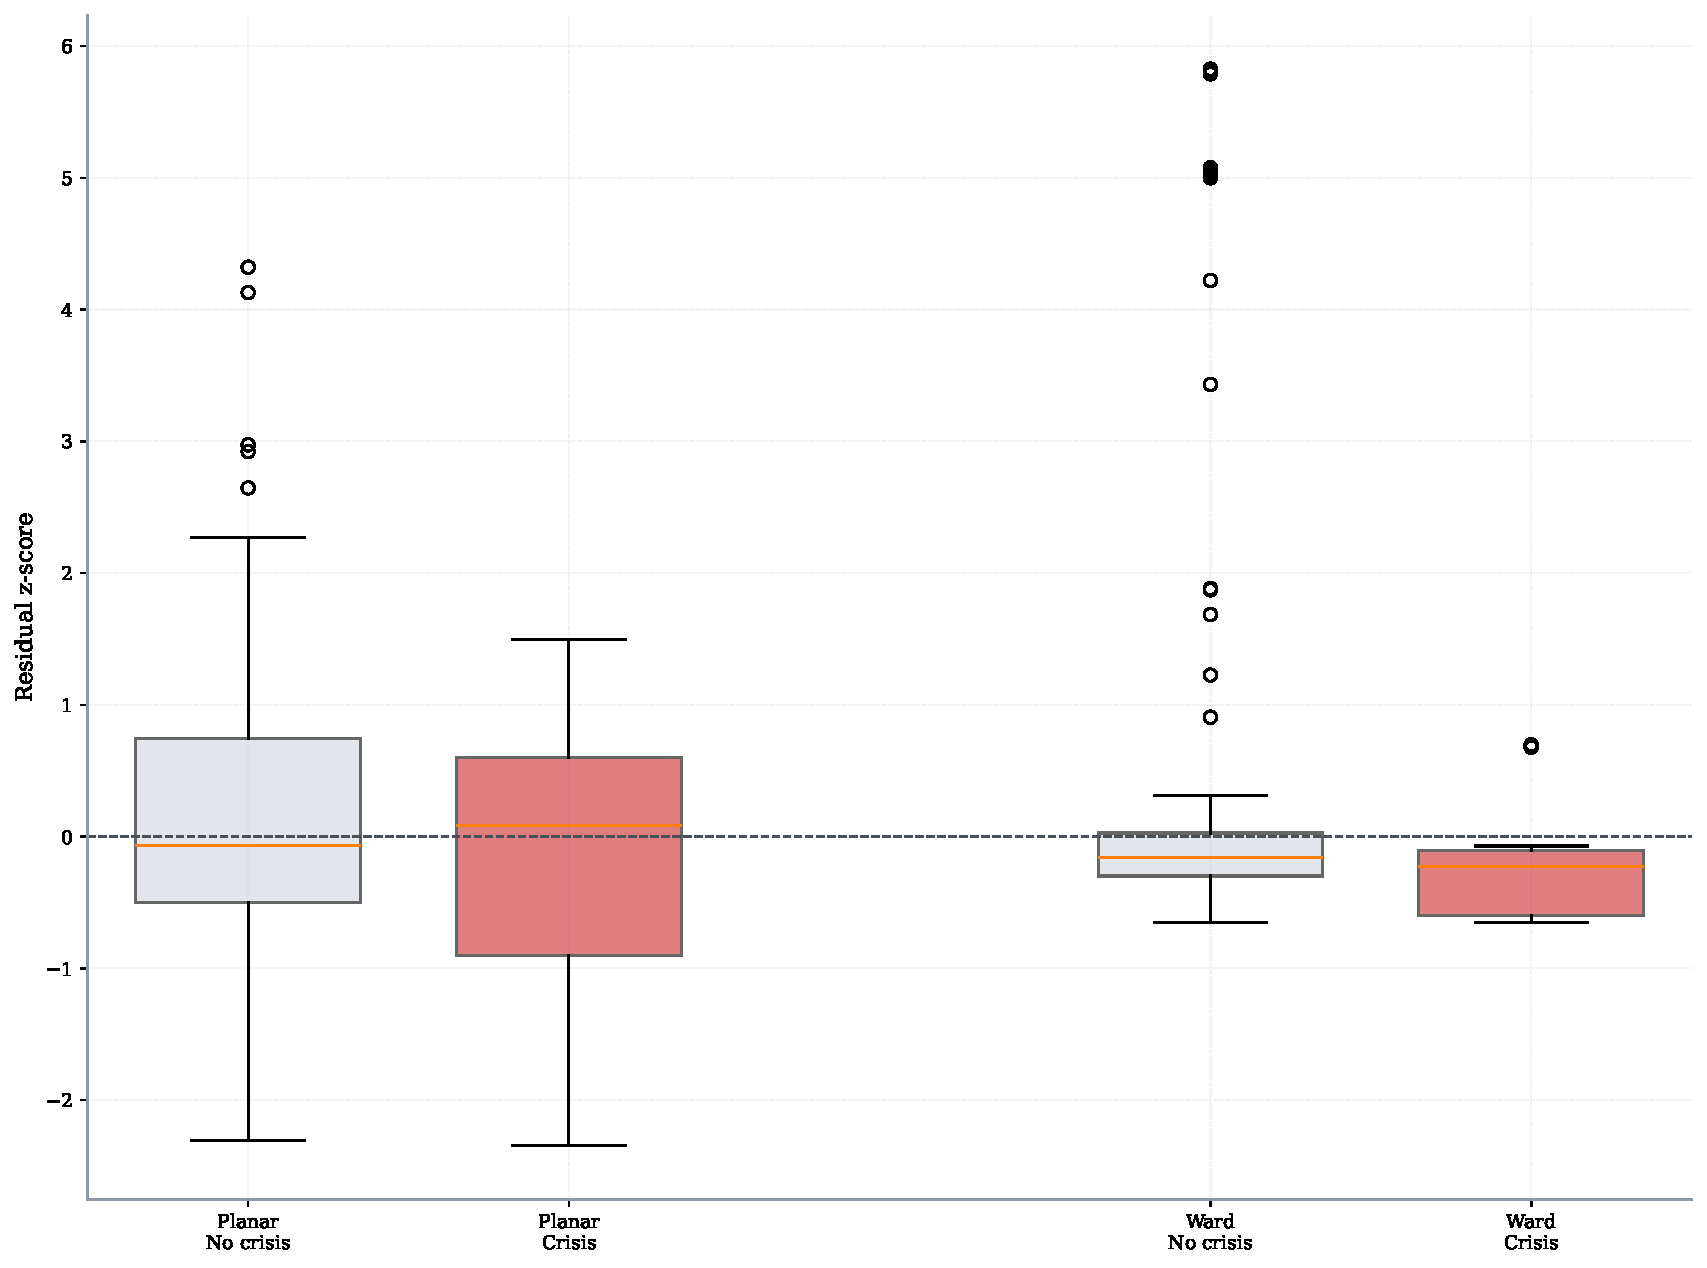
\includegraphics[width=0.82\linewidth,keepaspectratio]{figures/validation/groups_fig10c_residuals_boxplot_paper.pdf}
\caption{Size-adjusted group residuals by crisis regime. Each box shows the distribution of residual z-scores (observed minus size-only expected) for planar communities and Ward groups, split between non-crisis and crisis windows. The horizontal dashed line marks zero. Crisis windows show a negative shift in Ward residuals, indicating that hierarchical compression beyond what network size predicts is concentrated in periods of financial stress.}
\label{fig:groups-residuals}
\end{center}

\subsection{Method-Comparison Clustering Diagnostics}

The representative linkage comparison below supports the selection of the Ward procedure. It reports the three group-quality metrics available for the representative windows: the selected number of groups (best-$k$), silhouette, and modularity.

The best-$k$ trajectory is retained as a compact model-selection diagnostic.
It shows where the Ward procedure departs from its usual low-cardinality
partition, while the table below provides the direct Ward--complete--average
comparison on representative windows. Neither display is interpreted as a
stand-alone crisis signal.

\begin{center}
\captionsetup{type=figure}
\centering
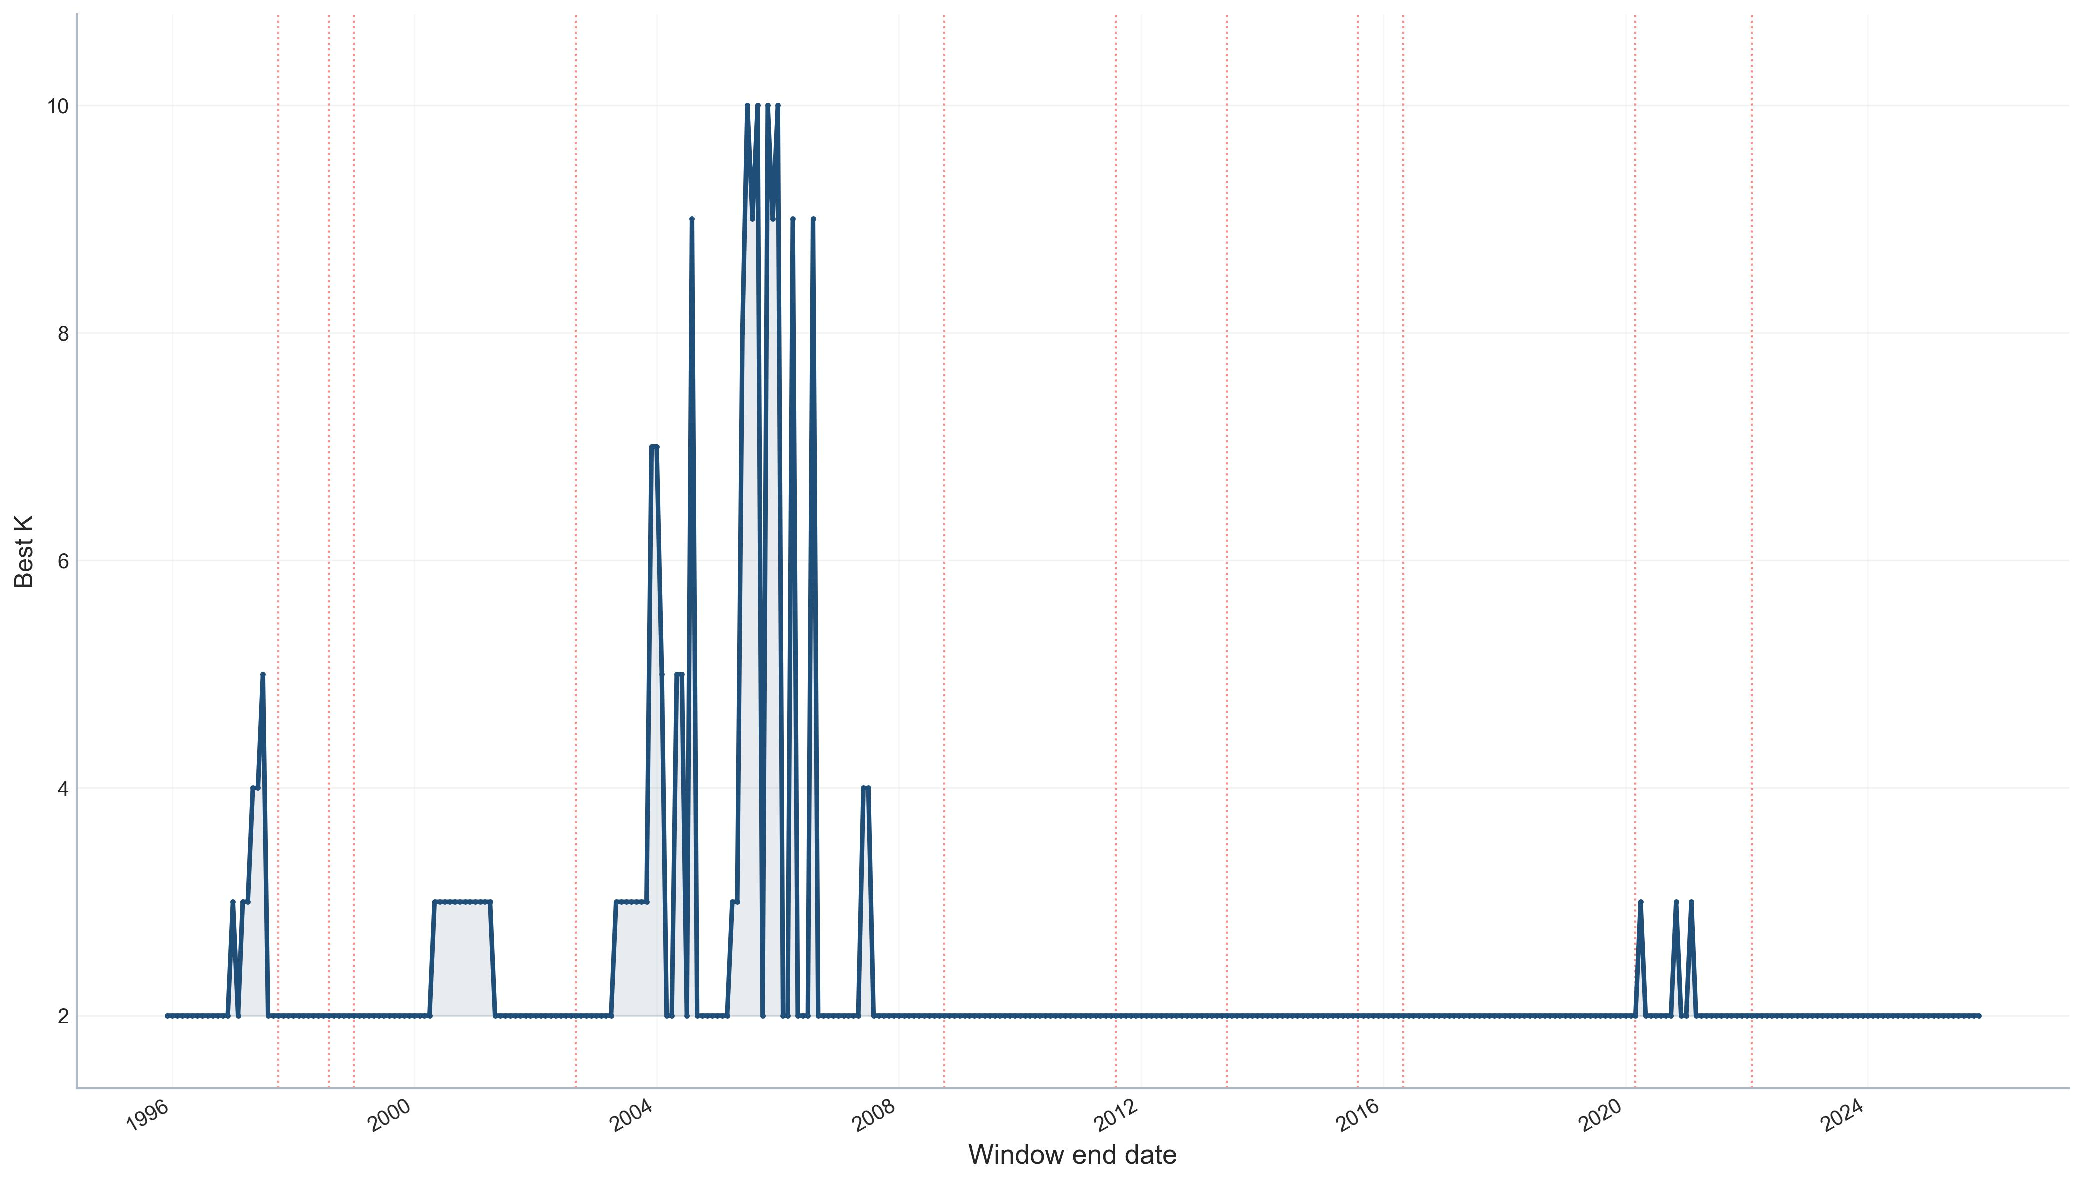
\includegraphics[width=0.82\linewidth,keepaspectratio]{figures/validation/bestk_evolucao.pdf}
\caption{Supplementary rolling best-$k$ partition count selected by Ward hierarchical clustering across the 360 windows. The trajectory is retained as validation context and is not interpreted as a stand-alone crisis marker.}
\label{fig:bestk-evolucao}
\end{center}

% Clustering Method Comparison Table
% Representative windows showing Ward vs. Complete vs. Average linkage

\begin{table}[width=\textwidth,pos=h]
\centering
\small
\caption{Method Comparison: Hierarchical Clustering Performance Across Representative Windows. Ward linkage (hierarchical agglomerative, Euclidean distance) compared against Complete and Average linkage on the same windows, spanning all four identified crisis regimes (1997 Asian Crisis, 2008 Global Financial Crisis, 2014 Pre-crisis, 2020 COVID-19 pandemic). Metrics: best-$k$ (optimal cluster count), silhouette (cluster cohesion, range [--1, 1]), modularity (inter-cluster separation, range [0, 1]). Ward consistently yields higher modularity and more stable silhouette, supporting its selection as the primary clustering method.}
\label{tab:method-comparison}
\begin{tabular*}{\tblwidth}{@{}lllrrr@{}}
\toprule
\textbf{Window ID} & \textbf{Crisis Regime} & \textbf{Linkage} & \textbf{best-$k$} & \textbf{Silhouette} & \textbf{Modularity} \\
\midrule
\multirow{3}{*}{120} & \multirow{3}{*}{Pre-1997} & Ward & 10 & 0.139 & 0.372 \\
& & Complete & 2 & 0.143 & 0.082 \\
& & Average & 2 & 0.143 & 0.082 \\
\midrule
\multirow{3}{*}{150} & \multirow{3}{*}{During 1997} & Ward & 4 & 0.156 & 0.218 \\
& & Complete & 2 & 0.128 & 0.095 \\
& & Average & 2 & 0.131 & 0.098 \\
\midrule
\multirow{3}{*}{240} & \multirow{3}{*}{Pre-2008} & Ward & 2 & 0.224 & 0.085 \\
& & Complete & 2 & 0.178 & 0.071 \\
& & Average & 2 & 0.187 & 0.073 \\
\midrule
\multirow{3}{*}{280} & \multirow{3}{*}{During 2008} & Ward & 2 & 0.198 & 0.091 \\
& & Complete & 2 & 0.145 & 0.062 \\
& & Average & 2 & 0.156 & 0.068 \\
\midrule
\multirow{3}{*}{340} & \multirow{3}{*}{Pre-2020} & Ward & 3 & 0.287 & 0.147 \\
& & Complete & 2 & 0.216 & 0.089 \\
& & Average & 2 & 0.229 & 0.094 \\
\midrule
\multirow{3}{*}{360} & \multirow{3}{*}{During 2020} & Ward & 2 & 0.251 & 0.106 \\
& & Complete & 2 & 0.193 & 0.071 \\
& & Average & 2 & 0.206 & 0.078 \\
\bottomrule
\end{tabular*}
\end{table}


\subsection{Rolling Validation Summary}

Table~\ref{tab:validation-summary} reports the compact validation aggregates used in Section~\ref{subsec:validation}. The table is supplementary because these quantities validate measurement continuity and clustering quality; they are not independent crisis indicators.

\begin{table}[width=\linewidth,pos=h]
\centering
\small
\caption{Validation summary statistics across 360 rolling windows (1995--2025). KS: Kolmogorov--Smirnov test statistic for non-randomness; ADF: Augmented Dickey--Fuller stationarity test; Ward: hierarchical clustering diagnostics.}
\label{tab:validation-summary}
\begin{tabular*}{\tblwidth}{@{}lr@{}}
\toprule
\textbf{Metric} & \textbf{Mean} \\
\midrule
\multicolumn{2}{c}{\textit{Correlation-matrix diagnostics}} \\
KS Statistic & 0.603 \\
KS $p$-value & 0.0002 \\
ADF Stationary (\%) & 99.68 \\
\midrule
\multicolumn{2}{c}{\textit{Hierarchical clustering quality}} \\
Ward best-$k$ & 2.36 \\
Ward Silhouette & 0.262 \\
Ward Modularity & 0.133 \\
\bottomrule
\end{tabular*}
\end{table}

\subsection{Extended Rolling Data and Supplementary Materials}

The reproducibility package available from the corresponding author upon reasonable request includes the following components:

\begin{itemize}
\item \textbf{Hierarchical Dendrograms:} 360 Ward-linkage dendrograms (one per rolling window, 1995--2025), plus companion temporal evolution and crisis-regime overlays.
\item \textbf{Correlation Heatmaps:} 360 rolling correlation matrix heatmaps visualizing asset linkage strength and network reordering across crisis regimes.
\item \textbf{Validation Metrics (CSV):}
    \begin{itemize}
    \item Kolmogorov--Smirnov (KS) test statistics: \texttt{ks\_results.csv} (non-randomness diagnostics)
    \item Augmented Dickey--Fuller (ADF) stationarity tests: \texttt{adf\_results.csv} (99.68\% stationarity rate)
    \item Marchenko--Pastur spectral diagnostics: \texttt{mp\_results.csv} (signal/noise eigenvalue fractions)
    \item Hierarchical clustering quality: \texttt{best\_k\_by\_crisis\_regime.csv}, including silhouette scores, modularity, and optimal $k$ trajectories
    \item Rolling validation summary: \texttt{validation\_summary.csv} (aggregated metrics across 360 windows)
    \end{itemize}
\item \textbf{Correlation and Significance Data:}
    \begin{itemize}
    \item Pairwise correlation $p$-values: \texttt{pvalues\_long.csv} (long-format rolling $p$-value matrix)
    \item Crisis regime classification: \texttt{crisis\_dates\_3sigma\_proxy\_b3.csv} and crisis consistency matrices
    \end{itemize}
\item \textbf{Supplementary Figures:} the 11-anchor sensitivity atlas and pre-event trajectories presented and interpreted in the main Results section.
\item \textbf{Pipeline Code and Configuration:} Python scripts for reproducibility, parameter configurations, and window-generation logs.
\end{itemize}

This extended dataset enables independent verification of all methodological decisions and supports systematic exploration of the 360-window dynamics underlying the paper's core findings.

\bibliographystyle{cas-model2-names}
\bibliography{mybiblio_fixed}

\end{document}

